\documentclass[aspectratio=169,xcolor=table]{beamer}
\usepackage{epstopdf}
\usepackage{textgreek}
\usepackage{physics}
\usepackage{appendixnumberbeamer}
\usepackage{multicol}
\usepackage{pbox}
\usepackage{amssymb}
\usepackage{xcolor}
\usepackage{blindtext}
\usepackage{color, colortbl}
\usepackage{xspace}
\usepackage{listings}
\usepackage{tikz}
\usepackage{variable_defs}
\usepackage{pifont}
\usepackage{subcaption}
\usetheme{NIU}
\usepackage{graphicx}
\graphicspath{{/Users/eparrish/Work/thesis/}}
\usepackage[style=ieee]{biblatex}
\setbeamertemplate{bibliography item}{\insertbiblabel}
\addbibresource{biblio.bib}
\usepackage{caption}
\captionsetup[figure]{labelformat=empty}% redefines the caption setup of the figures environment in the beamer class.

% \bibliography{biblio.bib}

% suppress navigation bar
\beamertemplatenavigationsymbolsempty

% Title
\title[Search for \HpmLong with ATLAS]
{Search for Charged Higgs Bosons in the \taulep Final State with \LUMI of \pp Collision Data at \sqs with the ATLAS Experiment}

% Sub Title
\subtitle{Dissertation Defense}

% Author
\author[Elliot Parrish]
{\texorpdfstring{\underline{Elliot Parrish}}{Elliot Parrish}}
\hypersetup{pdfauthor={Elliot Parrish}}

% - Give the names in the same order as the appear in the paper.
% - Use \and to separate authors name
% - Use the \inst{?} command only if the authors have different affiliation.

\institute[NIU] {\inst{\dag}Northern Illinois University, USA}
% \institute[IFJ PAN] {}
% - Use the \inst command only if there are several affiliations.
% - Keep it simple, no one is interested in your street address.

\date{October 13, 2022}
% \subject{} % only for pdf info

% if you want to disable section, subsection title page display, uncomment accordingly 
\AtBeginSection[]{
  \begin{frame}
  \vfill
  \centering
  \begin{beamercolorbox}[sep=8pt,center,shadow=true,rounded=true]{title}
    \usebeamerfont{title}\insertsectionhead\par%
  \end{beamercolorbox}
  \vfill
  \end{frame}
}
\AtBeginSubsection{}

% Title Graphics add befor titlepage
\titlegraphic{
\includegraphics[height=2.5cm]{NIU_logo.eps}}

\newcommand{\specialcell}[2][l]{%
  \begin{tabular}[#1]{@{}l@{}}#2\end{tabular}}

\newcommand{\Cross}{$\mathbin{\tikz [x=1.4ex,y=1.4ex,line width=.2ex, red] \draw (0,0) -- (1,1) (0,1) -- (1,0);}$}%
% \newcommand{\Hp}{\ensuremath{H^{\pm}}\xspace}
% \newcommand{\Etm}{\ensuremath{E_\text{T}^\text{miss}}\xspace}
% \newcommand{\pt}{\ensuremath{p_\text{T}}\xspace}
% \newcommand{\HpmLong}{\ensuremath{\Hp \rightarrow \tau \nu}\xspace}

\begin{document}
\frame{\titlepage}

% add logo after title page, so it does show on title page
\logo{
\includegraphics[trim=1cm 2.5cm 1cm 0,clip,width=1.3cm,keepaspectratio=true]{NIU_logo.eps}}
% \logo{\includegaraphics}


% Table of Contents
% \begin{frame}<beamer>{Table of Contents}
%     \tableofcontents
% \end{frame}

\begin{frame}{\contentsname}
  \begin{multicols}{2}
    \tableofcontents
  \end{multicols}
\end{frame}

\section{Introduction }
  
  \begin{frame}[t]{Welcome}
    \begin{itemize}
      \item This defense will take $\sim 1$ hour
      \begin{itemize}
        \item I will walk you through the work that is contained in my PhD dissertation
        \item After the presentation is complete, the committee and I will address comments privately
        \item When we are done, I will return, the committee will discuss among themselves then return
      \end{itemize}
      \item General Guidelines
      \begin{itemize}
        \item Please remain muted unless you are speaking
        \item There will be time at the end for questions, but feel free to interrupt if there is something urgent
      \end{itemize}
      \item Thank you for attending!
    \end{itemize}
  \end{frame}

\section{Theory }
  
  \subsection{The Standard Model }
  \begin{frame}[t]{What are we made of?}
    \begin{columns}
    \column{.59\textwidth}
      \begin{itemize}
        \item The scientific field of particle physics seeks to explain the building blocks of the universe
        \begin{itemize}
          \item How many fundamental particles are there?
          \item How do they interact with each other
        \end{itemize}
        \item The Standard Model of Particle Physics (SM)
        \begin{itemize}
          \item Matter is comprised of fermions
            \begin{itemize}
              \item Half-integer spin $(s=\frac{1}{2},\frac{3}{2},\frac{5}{2},etc.)$
              \item Anti-matter is identical to matter except for opposite electromagnetic charge
            \end{itemize}
          \item Forces are carried by an exchange of bosons
            \begin{itemize}
              \item Integer spin $(s=0,1,2,etc.)$
              \item Gluon (g) $\to$ Strong force
              \item Photon ($\gamma$) $\to$ Electromagnetism
              \item $W^{\pm},Z^{0}$ $\to$ Weak force
              % \item Higgs (H) $\to$ mass
            \end{itemize}
        \end{itemize}
      \end{itemize}
    \column{.4\textwidth}
      \begin{figure}
        \centering
        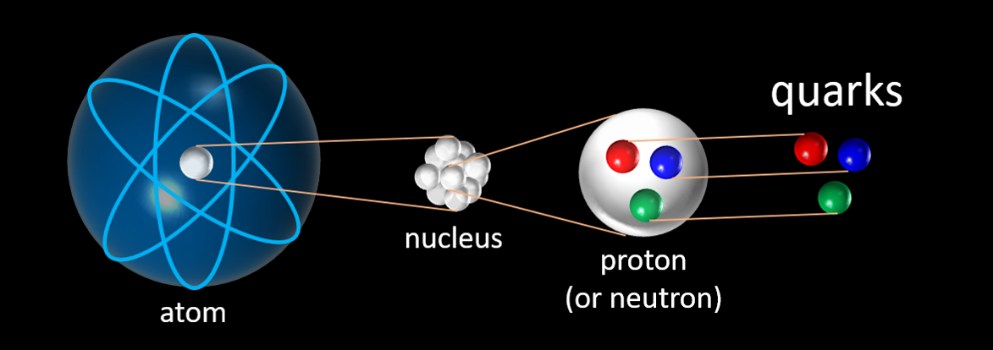
\includegraphics[width=\textwidth,keepaspectratio=true]{/Users/eparrish/Work/thesis/chapters/chapter2_theory/images/Atom_to_Quark_Cartoon.png}
        \caption{\tiny\cite{atom-to-quark}}
        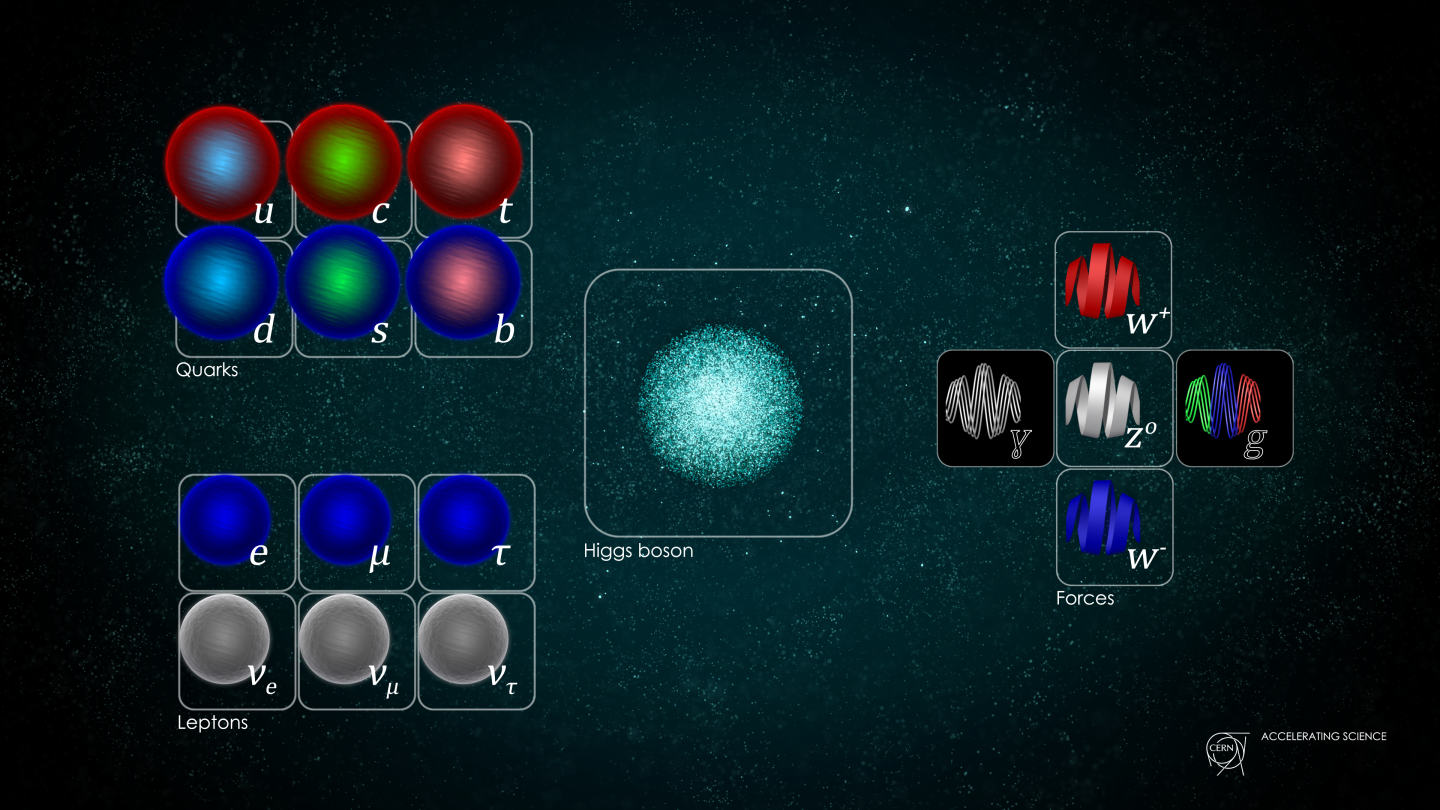
\includegraphics[width=\textwidth,keepaspectratio=true]{STDM higgs and field D.png}
      \end{figure}
    \end{columns}
  \end{frame}

  \subsection{Higgs Mechanism}

  \begin{frame}[t]{The Higgs Mechanism}
    \begin{columns}
    \column{.75\textwidth}
      \begin{itemize}
        \item Theorized by Higgs, Englert, and Brout in 1964
          \begin{itemize}
            \item Complex scalar doublet ($s=0$)
            \item Non-zero vacuum expectation value
          \end{itemize}
        \item Interactions with Higgs field give particles mass
        \item Discovered jointly by the ATLAS and CMS collaborations in 2012
      \end{itemize}
    \column{.25\textwidth}
      \begin{figure}
        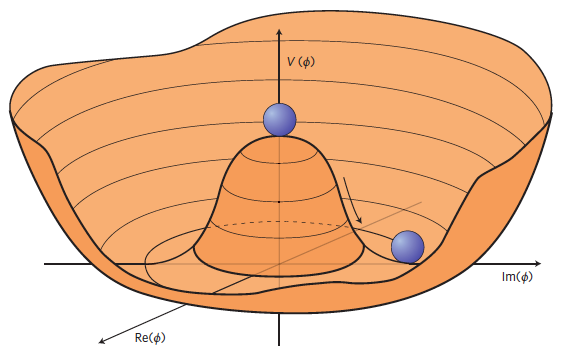
\includegraphics[width=.75\textwidth,keepaspectratio=true]{/Users/eparrish/Work/thesis/chapters/chapter2_theory/images/higgspotential.png}
        \caption{\tiny Higgs potential \cite{Higgs-phys}}
      \end{figure}
      \vspace{-.80cm}
      \begin{figure}
        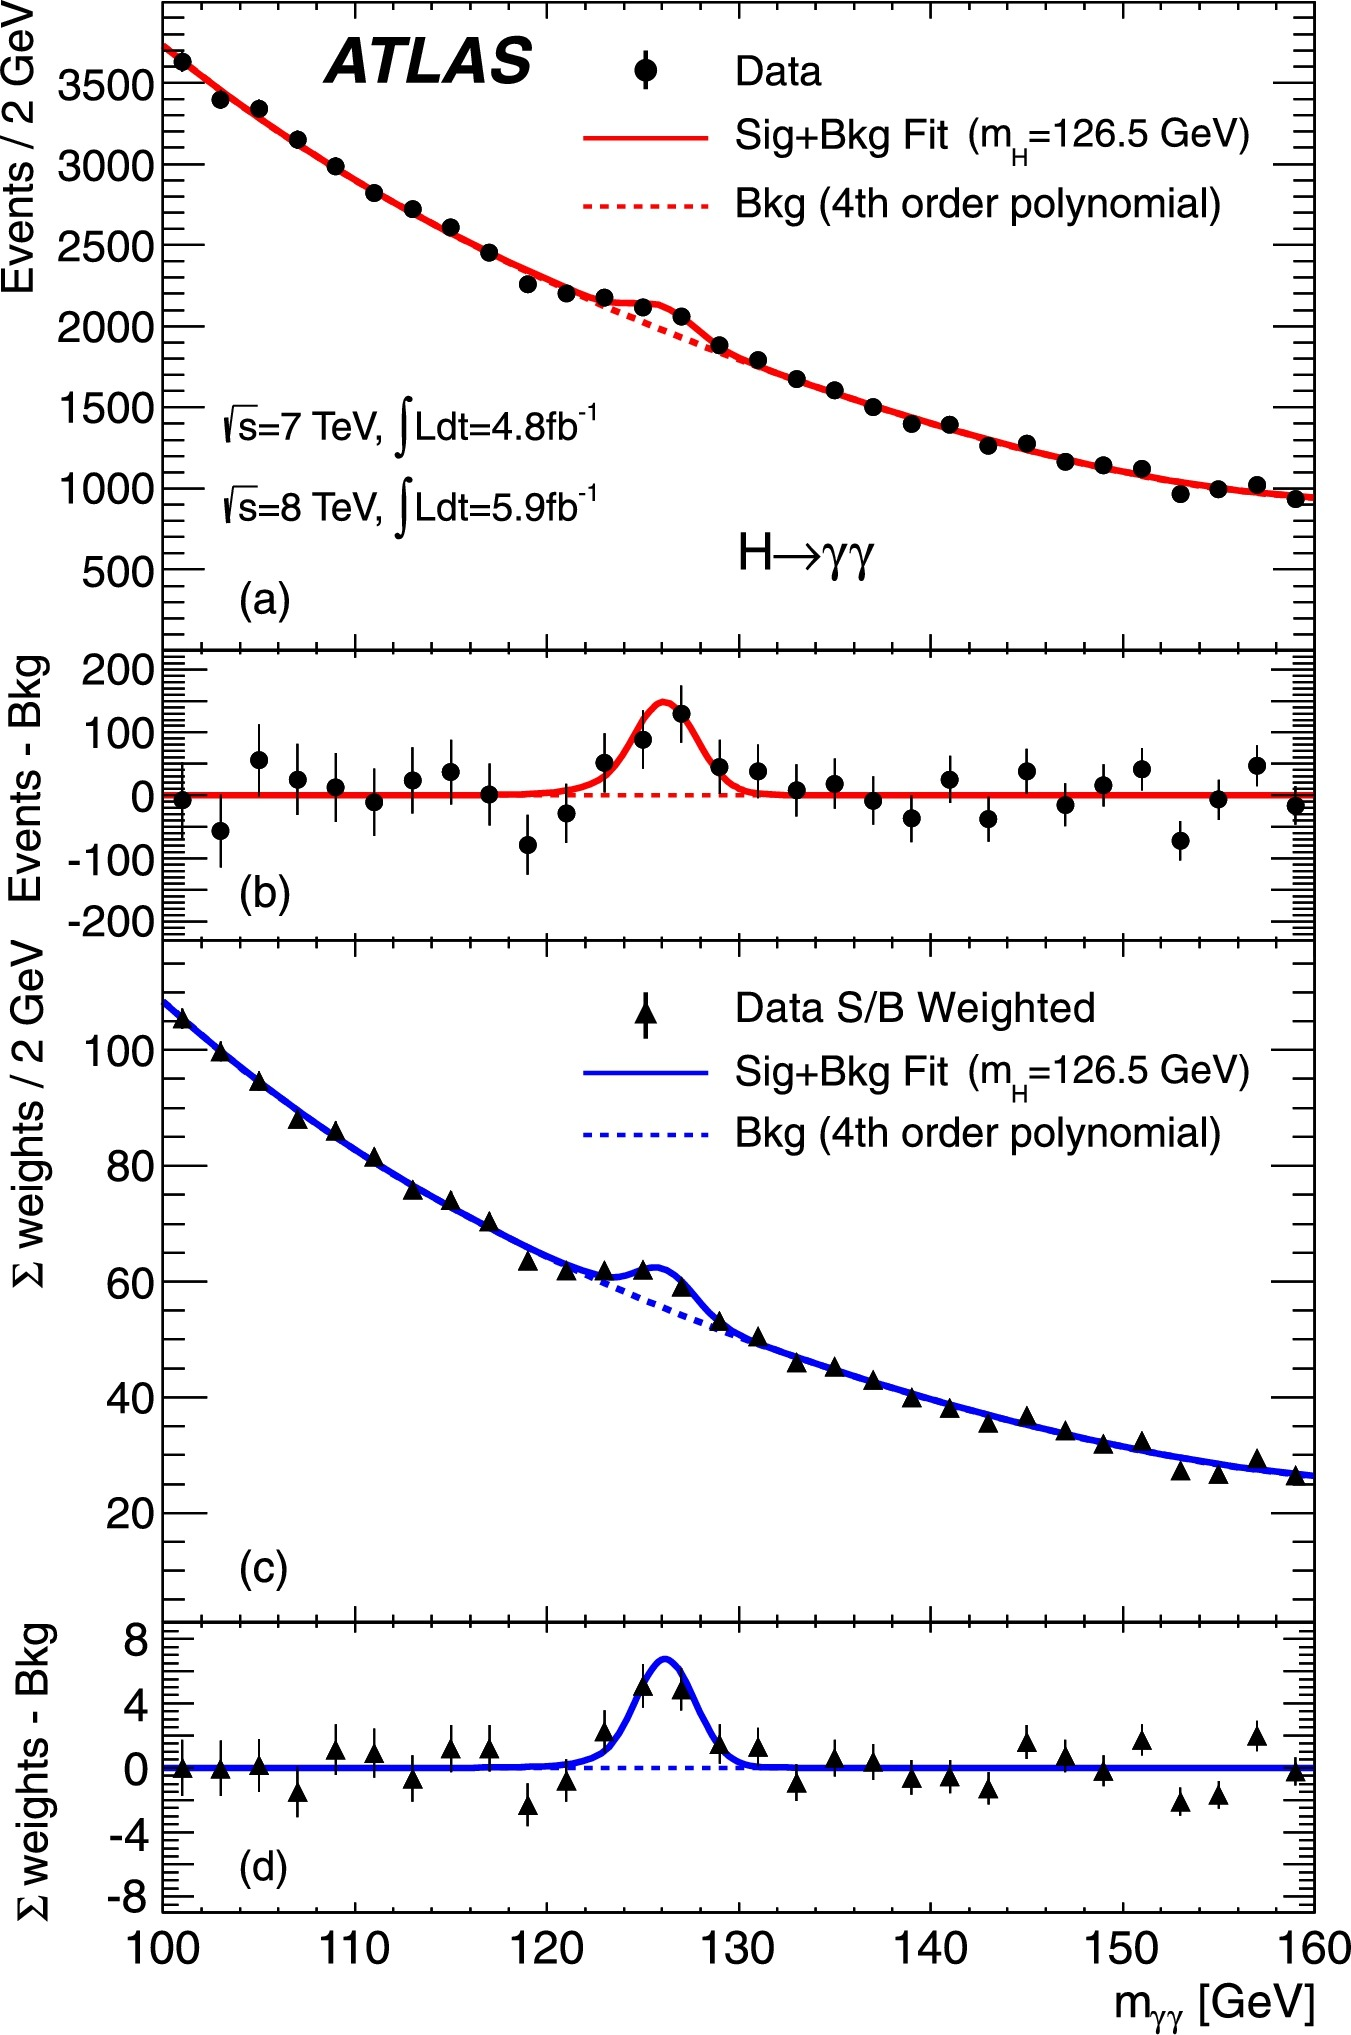
\includegraphics[height=.45\textheight,keepaspectratio=true]{/Users/eparrish/Work/thesis/chapters/chapter2_theory/images/Higgs_Discovery_gam_gam.jpeg}
        \caption{\tiny Higgs discovery \cite{higgs-discovery-atlas}}
      \end{figure}
    \end{columns}
  \end{frame}

  \begin{frame}[c]{The Standard Model}
    \begin{columns}
    \column{.45\textwidth}
      \small
      \begin{itemize}
        % \item Quantum field theory that explains the fundamental forces, particles, and their interactions
        \item Predicts the probabilities of particles decaying to others (among many other things)
        \begin{itemize}
          \item Has been thoroughly tested
          \item Measurements agree to a high degree of accuracy
        \end{itemize}
        \item Not a complete theory
        \begin{itemize}
          \item Gravity
          \item Matter-antimatter asymmetry in the universe
          \item Predicted neutrino masses are 0
          \begin{itemize}
            \item Observed neutrino mixing says otherwise
          \end{itemize}
        \end{itemize}
      \end{itemize}
    \column{.55\textwidth}
      \begin{figure}
        \centering
        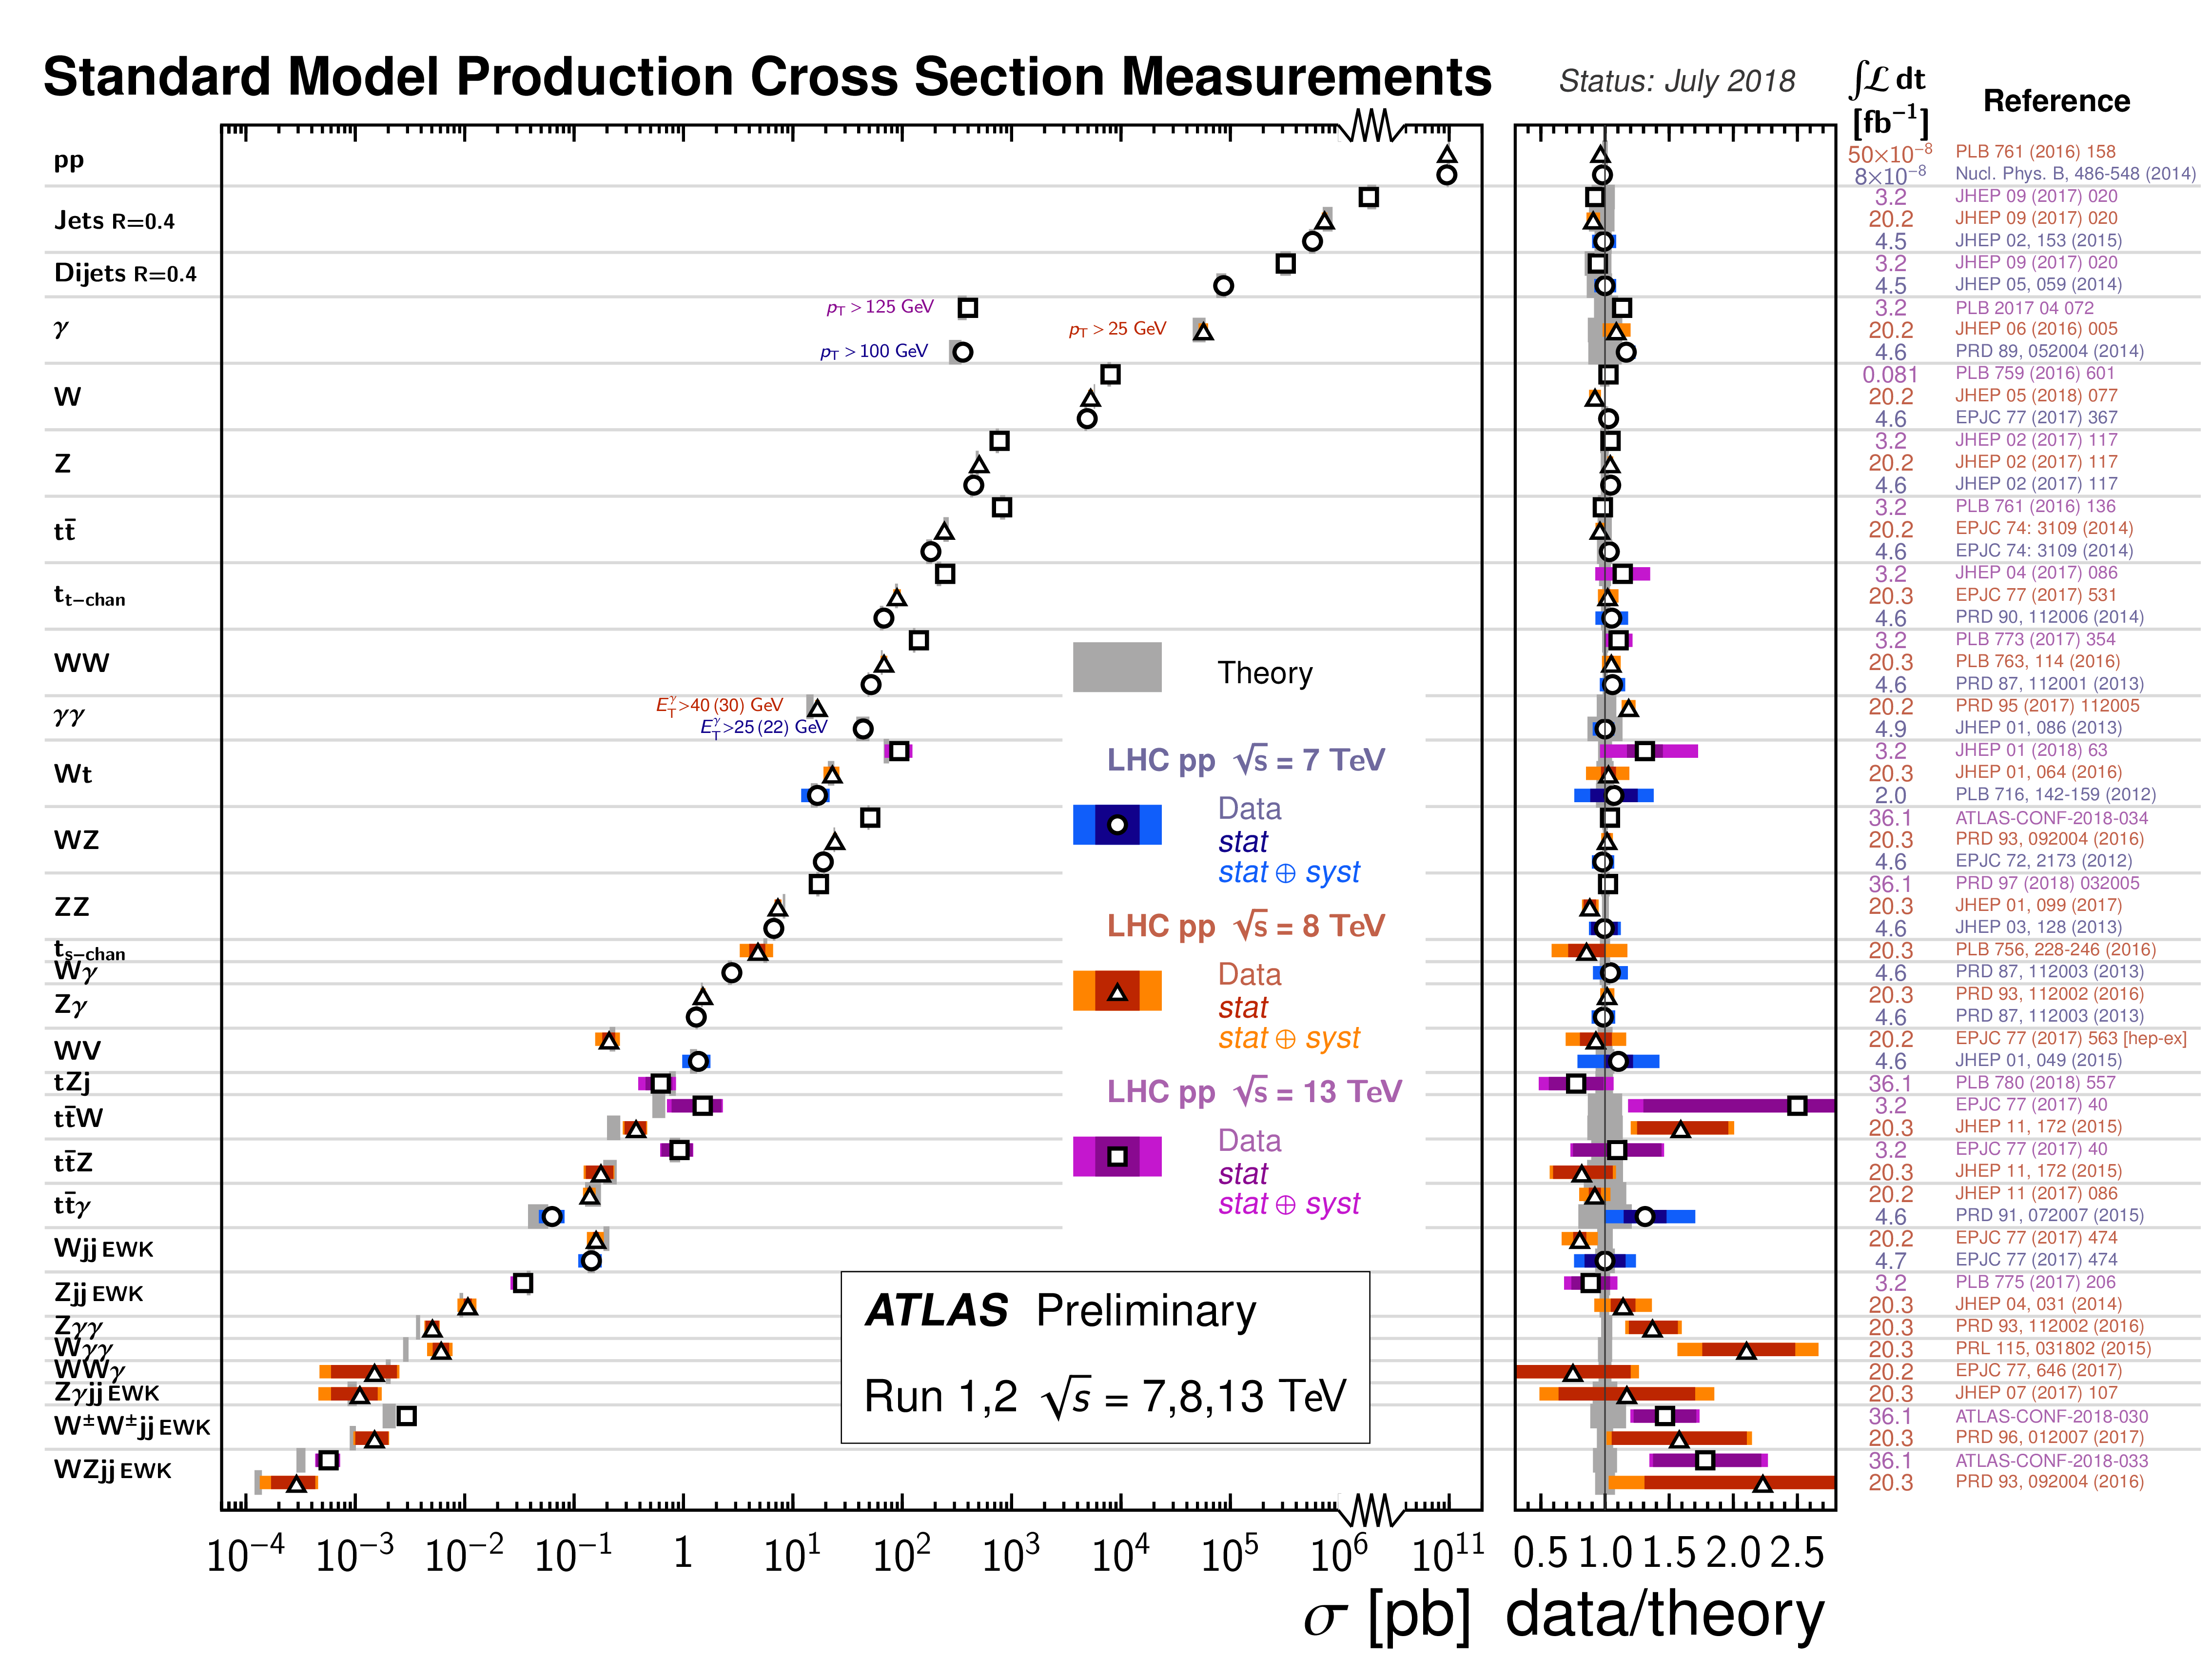
\includegraphics[width=\textwidth,keepaspectratio=true]{ATLAS_d_SMSummary_FiducialXsect_rotated.png}
        % \caption{\tiny}
      \end{figure}
    \end{columns}
  \end{frame}

  \subsection{Supersymmetry }

    \begin{frame}[t]{Supersymmetry}
      \begin{columns}
      \column{.8\textwidth}
        \begin{itemize}
          \item Hierarchy problem, ``unnaturalness''
          \begin{itemize}
            % \item Large Higgs mass terms cancel to give $\sim 125$ GeV
            \item Electroweak scale is $\sim 100$ GeV
            \item Planck scale is $\sim 2.4 \times 10^{18}$ GeV
            \item Supersymmetry (SUSY) offers many new particles to occupy the intermediate range
          \end{itemize}
          \item SUSY proposes a symmetry between fermions and bosons (spin)
          \begin{itemize}
            \item $Q | Fermion \rangle = | Boson \rangle$ 
            \item $Q | Boson \rangle = | Fermion \rangle$
          \end{itemize}
          \item SUSY is a large group of theories
          \begin{itemize}
            \item Minimal Supersymmetric Standard Model (MSSM) is the smallest SUSY extension to the SM
            \item 2 Higgs Doublet Models have two complex doublet scalar fields
            \begin{itemize}
              \item Two relevant free parameters, \tanb and \mHpm
              \item \tanb is the ratio of the vacuum expectation values of \Hpm
            \end{itemize}
          \end{itemize}
        \end{itemize}
      \column{.2\textwidth}
        \begin{table}[!thp]
          \centering
          \resizebox{\textwidth}{!}{
          \begin{tabular}{| l | c |}
          \hline
          light neutral scalar  & $h^0$ \\ \hline
          heavy neutral scalar  & $H^0$ \\ \hline
          neutral pseudoscalar  & $A^0$ \\ \hline
          two charged scalars   & \Hpm \\ \hline
          \end{tabular}}
          % \caption{\cite{2HDM}}
      \end{table}
      \end{columns}
    \end{frame}

  \subsection{Charged Higgs Bosons }

    \begin{frame}[t]{Charged Higgs Bosons}
      \begin{columns}
      \column{.75\textwidth}
      \begin{itemize}
        \item Many extensions to the Higgs sector imply the existence of charged scalars (2HDM, NMSMM, Triplet, etc.)
        \begin{itemize}
          \item \HpmLong remains significant for high \tanb
          % \begin{itemize}
          %   \item $\mathrm{tan} \beta$ defined as the ratio of the  vacuum expectation values of the two doublets
          % \end{itemize}
        \end{itemize}
        \item At the LHC, theoretical production mode of \mHpm is mainly in top-quark decays or in association with a top-quark ($t$)
        \begin{itemize}
          \item $H^{\pm}$ production mode is dependent on \mHpm
          \item Analysis is sensitive for low mass $(\mHpm < m_{t})$, intermediate mass $(\mHpm \simeq m_{t})$, and high mass $(\mHpm > m_{t})$
        \end{itemize}
        \item Two sub-channels based on the decay mode of associated $t$ 
        % \begin{itemize}
        %   \item $t \rightarrow jets$ 
        %     \begin{itemize}
        %       \item Sensitive at high mass due to higher $W \rightarrow q\bar{q}$ BR
        %     \end{itemize}
        %     \item $t \rightarrow \ell$
        %     \begin{itemize}
        %       \item Sensitive at low mass due to single lepton triggers
        %     \end{itemize}
        % \end{itemize}
      \end{itemize}
      \vspace{-.3cm}
      \centering
      \begin{table}
          % \small
          \resizebox{.9\textwidth}{!}{
          \rowcolors{1}{}{NIUgray}
          \begin{tabular}{c | c}
          \textbf{$t \rightarrow jets$ } & $t \to \ell$ \\
          \hline \hline
          Sensitive at high mass due to higher $W \to q\bar{q}$ BR & Sensitive at low mass due to single lepton triggers \\
          \end{tabular}}
        \end{table}

      \column{.25\textwidth}
      \centering
      % 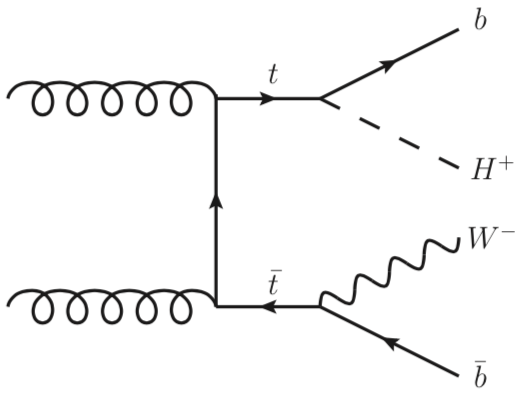
\includegraphics[width=.74\textwidth,keepaspectratio=true]{double_resonant_production_low_mass.png}
      % 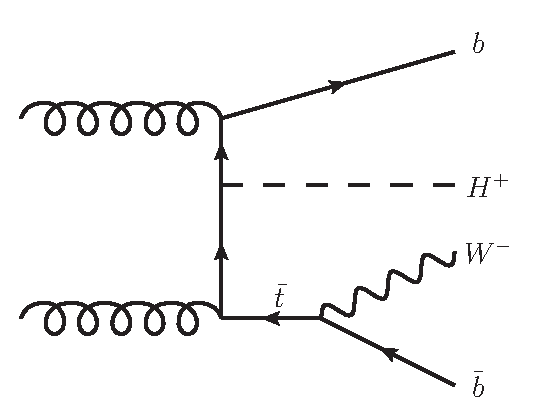
\includegraphics[width=.74\textwidth,keepaspectratio=true]{SingleResonant.pdf}
      % 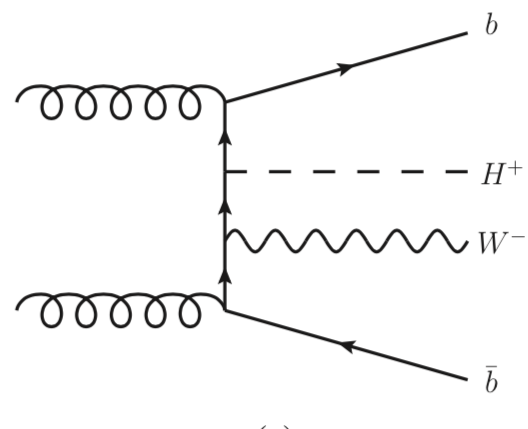
\includegraphics[width=.74\textwidth,keepaspectratio=true]{non_resonant_production_intermediate_mass.png}
      % 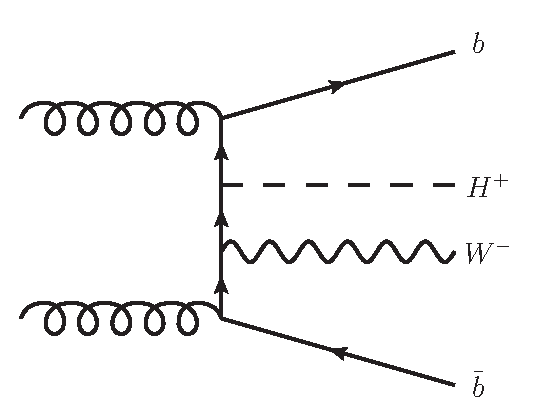
\includegraphics[width=.74\textwidth,keepaspectratio=true]{NonResonant.pdf}
      % 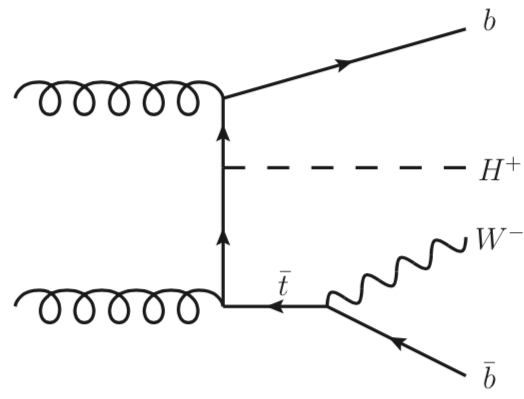
\includegraphics[width=.74\textwidth,keepaspectratio=true]{single_resonant_production_large_mass.png}
      % 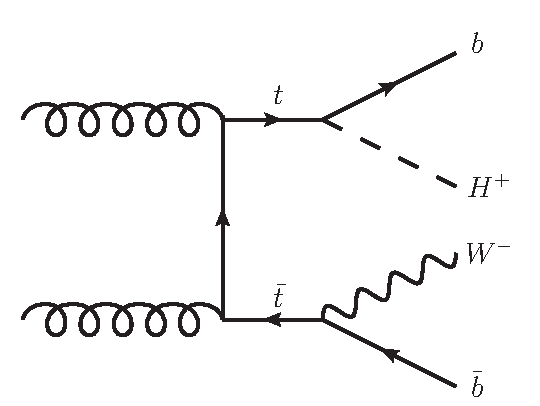
\includegraphics[width=.74\textwidth,keepaspectratio=true]{DoubleResonant.pdf}
      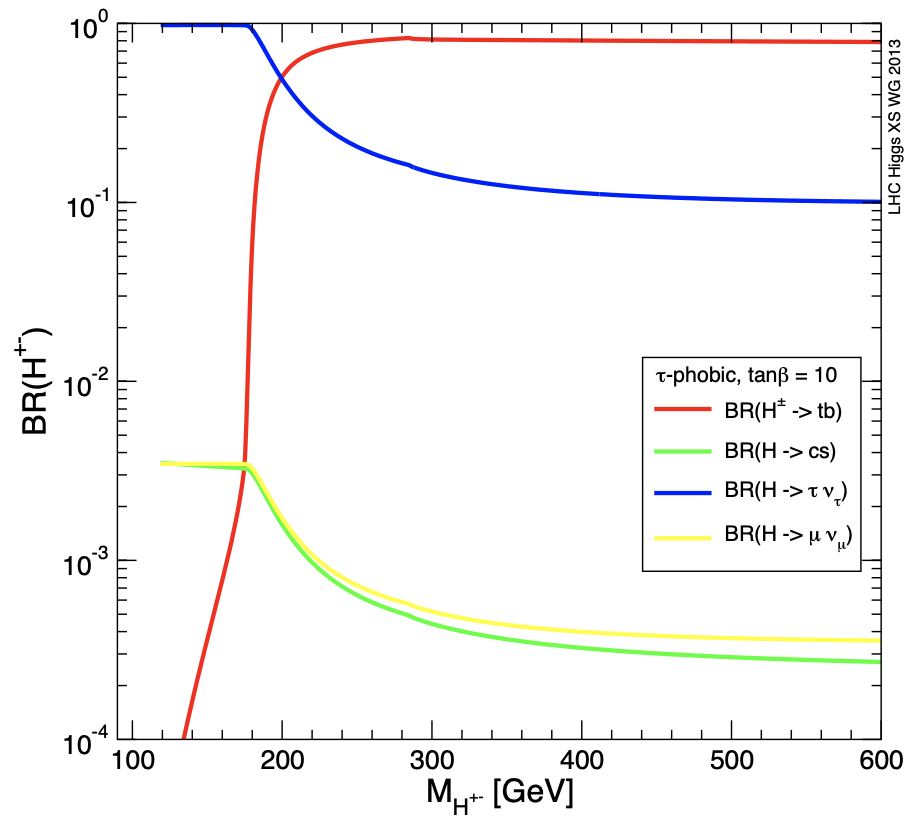
\includegraphics[width=1.15\linewidth,keepaspectratio=true]{Charged_Higgs_BR.png}
      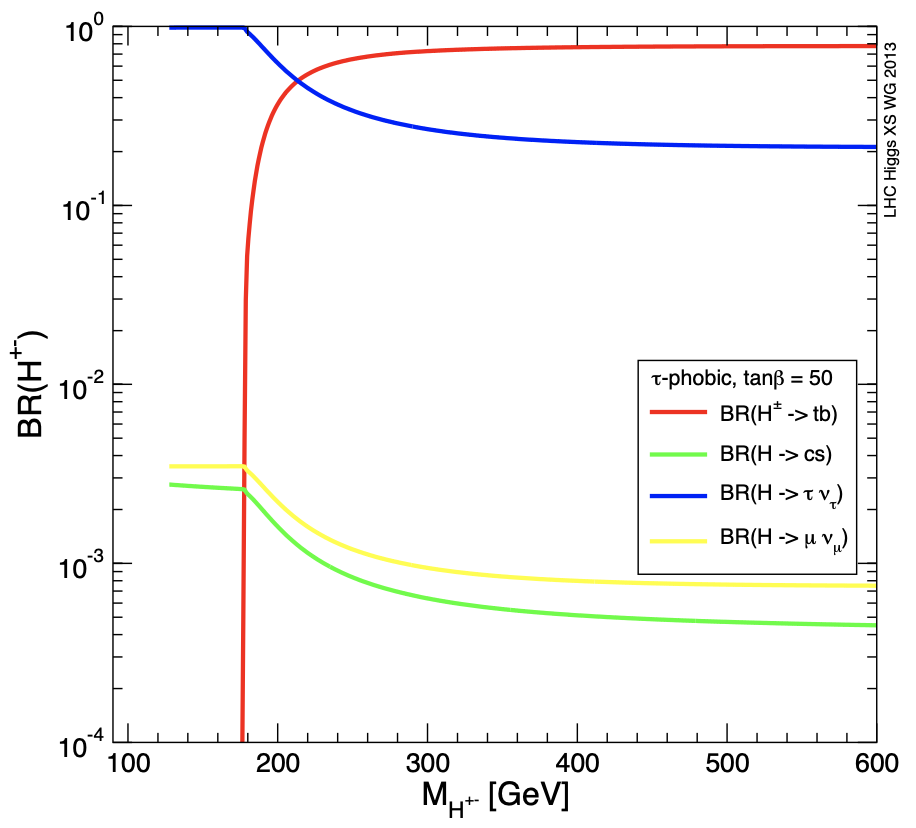
\includegraphics[width=1.15\linewidth,keepaspectratio=true]{HPlus_taunu_tanB.png}
      \end{columns}
    \end{frame} 


\begin{frame}[t]{\href{https://link.springer.com/article/10.1007/JHEP09(2018)139}{JHEP 09(2018)139} BDT Scores in Signal Regions}
        \begin{columns}[t]
          \column{.33\textwidth}
          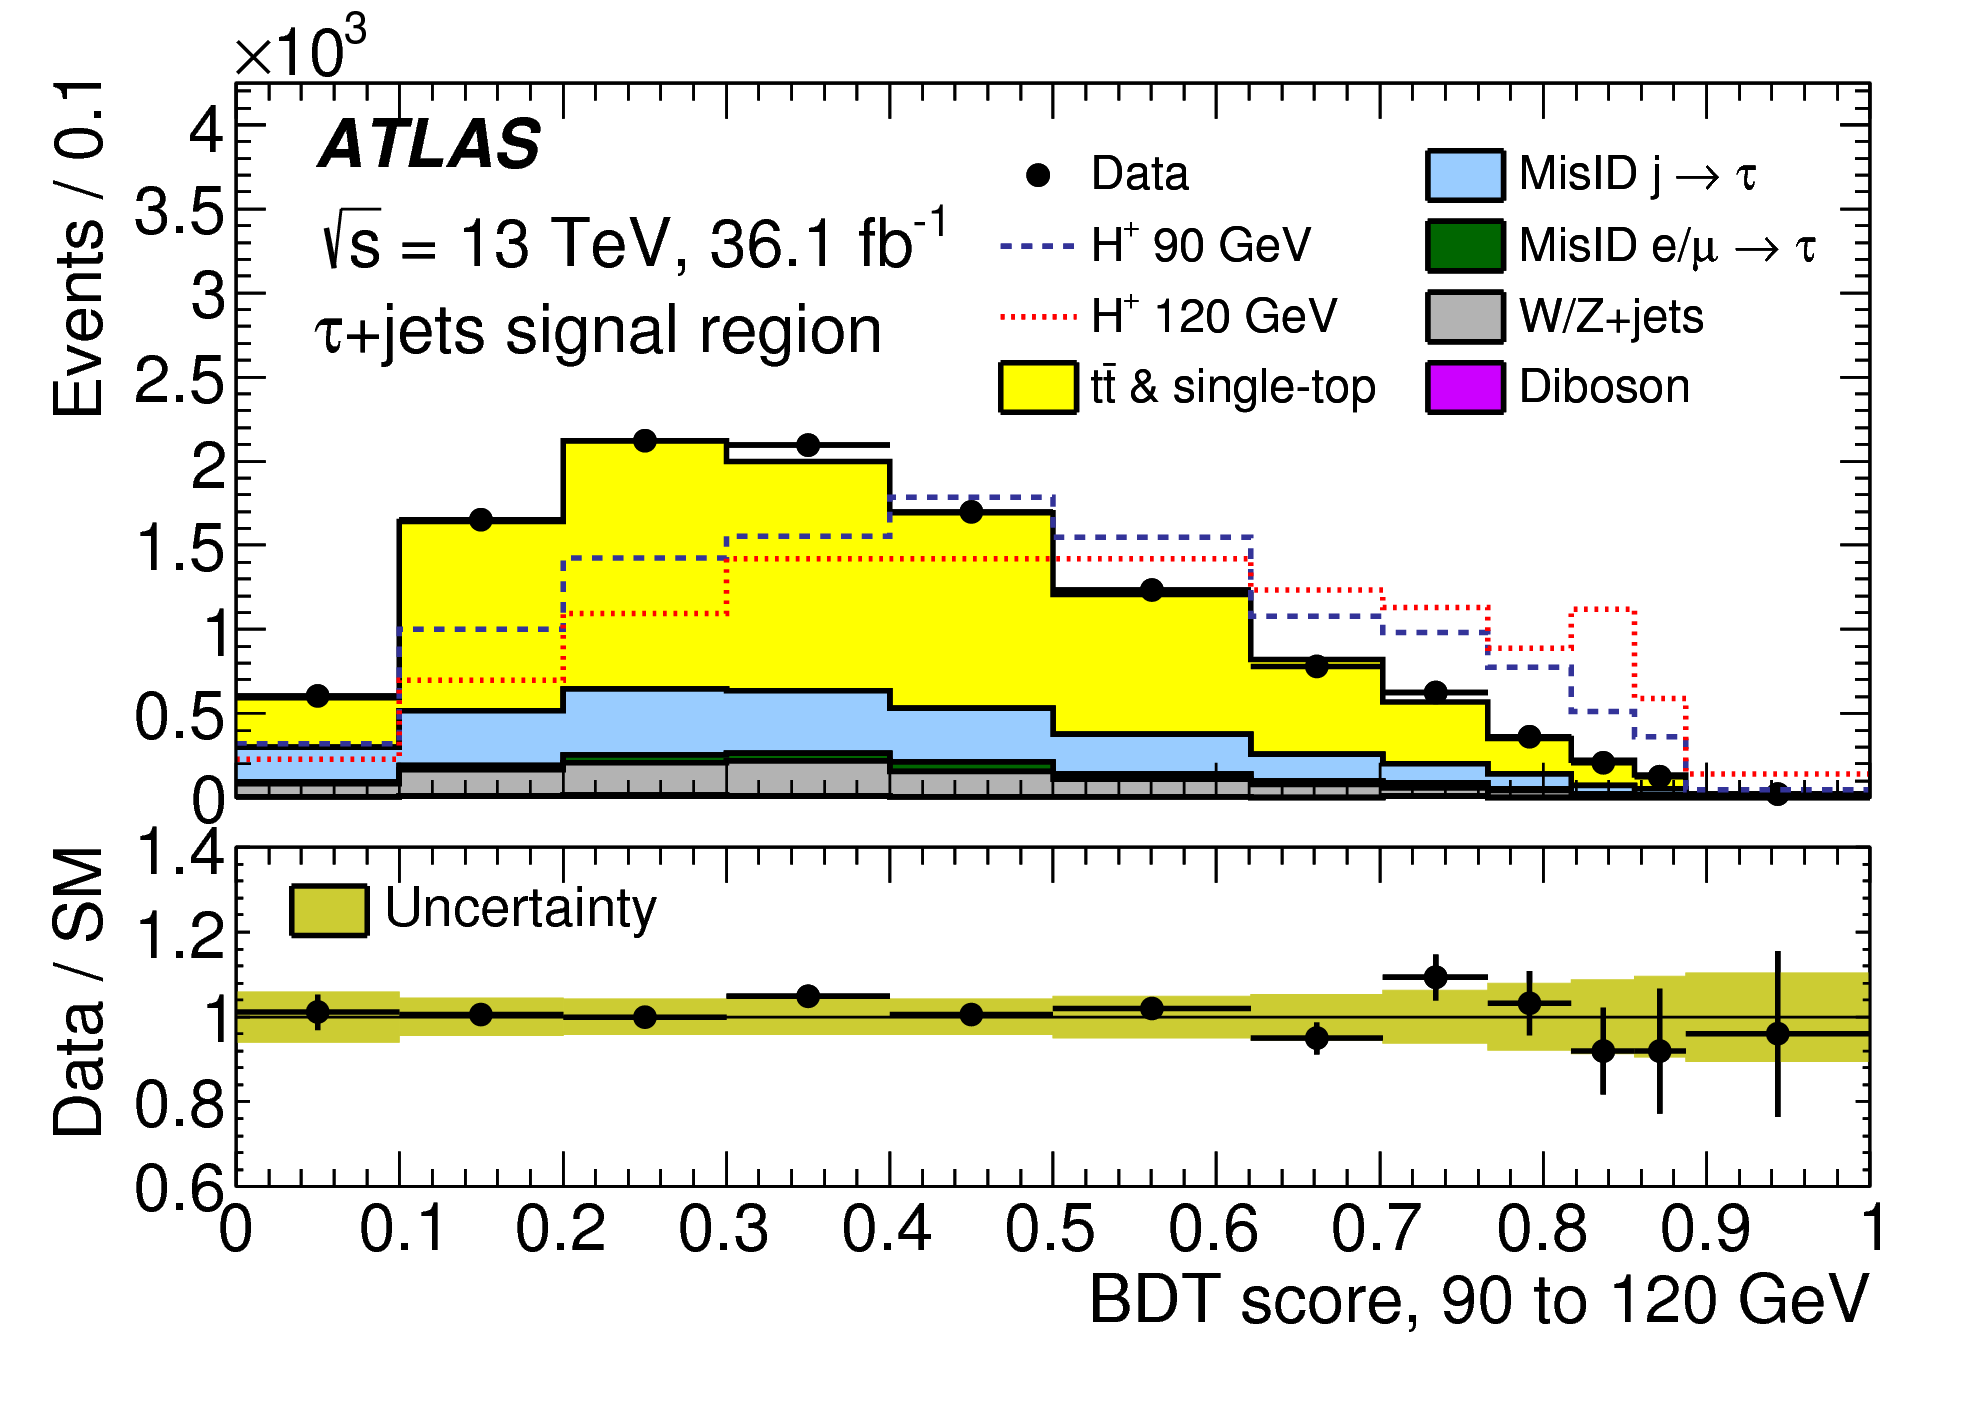
\includegraphics[height=.4\textheight,keepaspectratio=true]{taujet_SR_2018/taujet_SR_90to120_2018.png}
          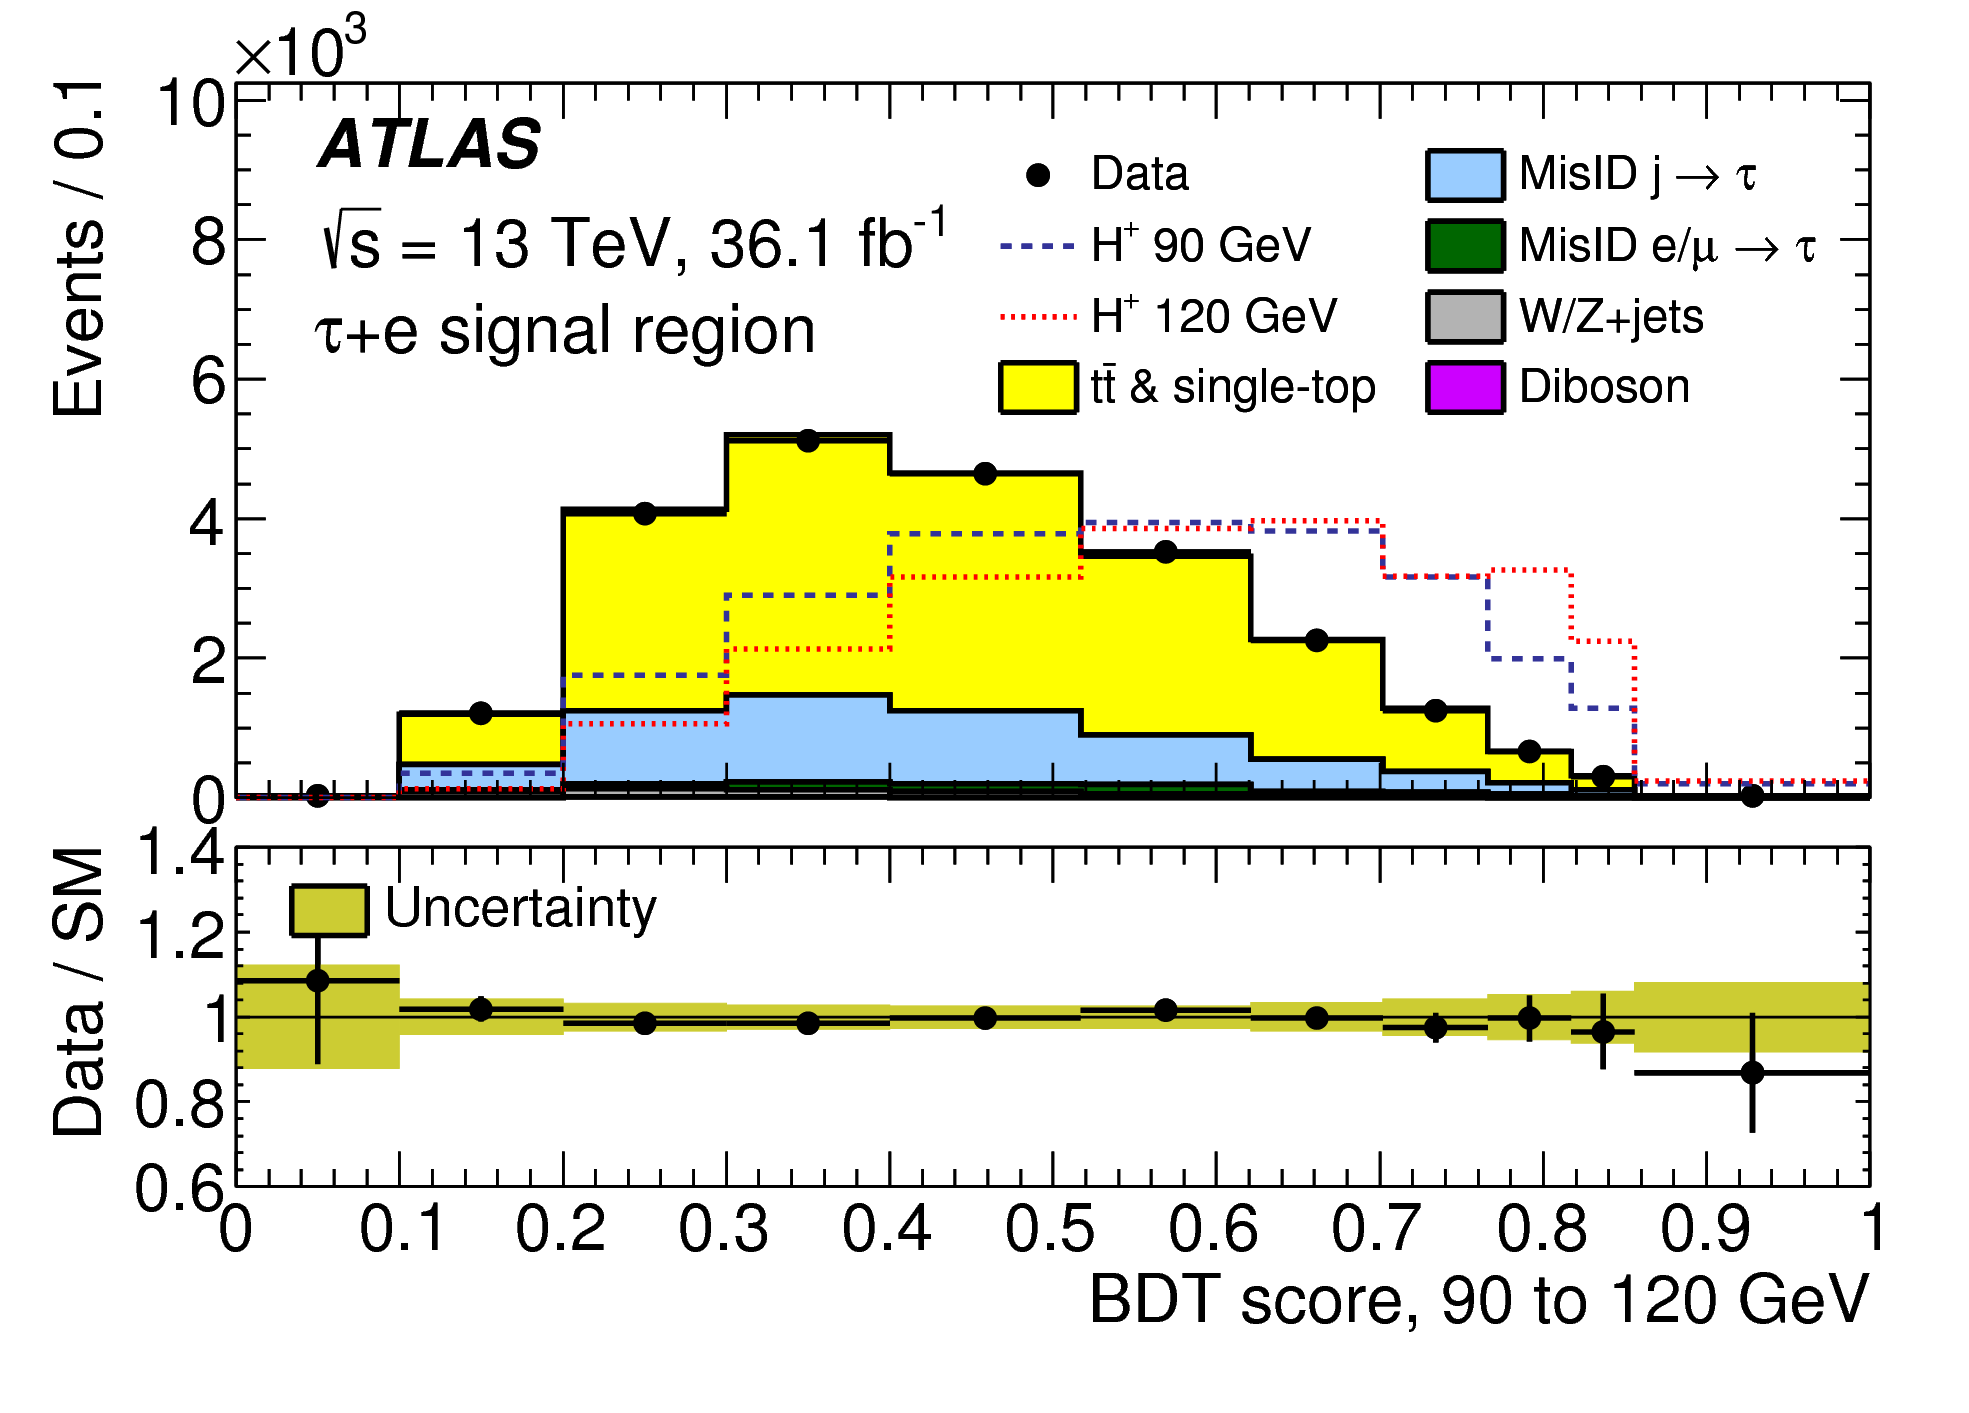
\includegraphics[height=.4\textheight,keepaspectratio=true]{tauel_SR_2018/tauel_SR_90to120_2018.png}
          % 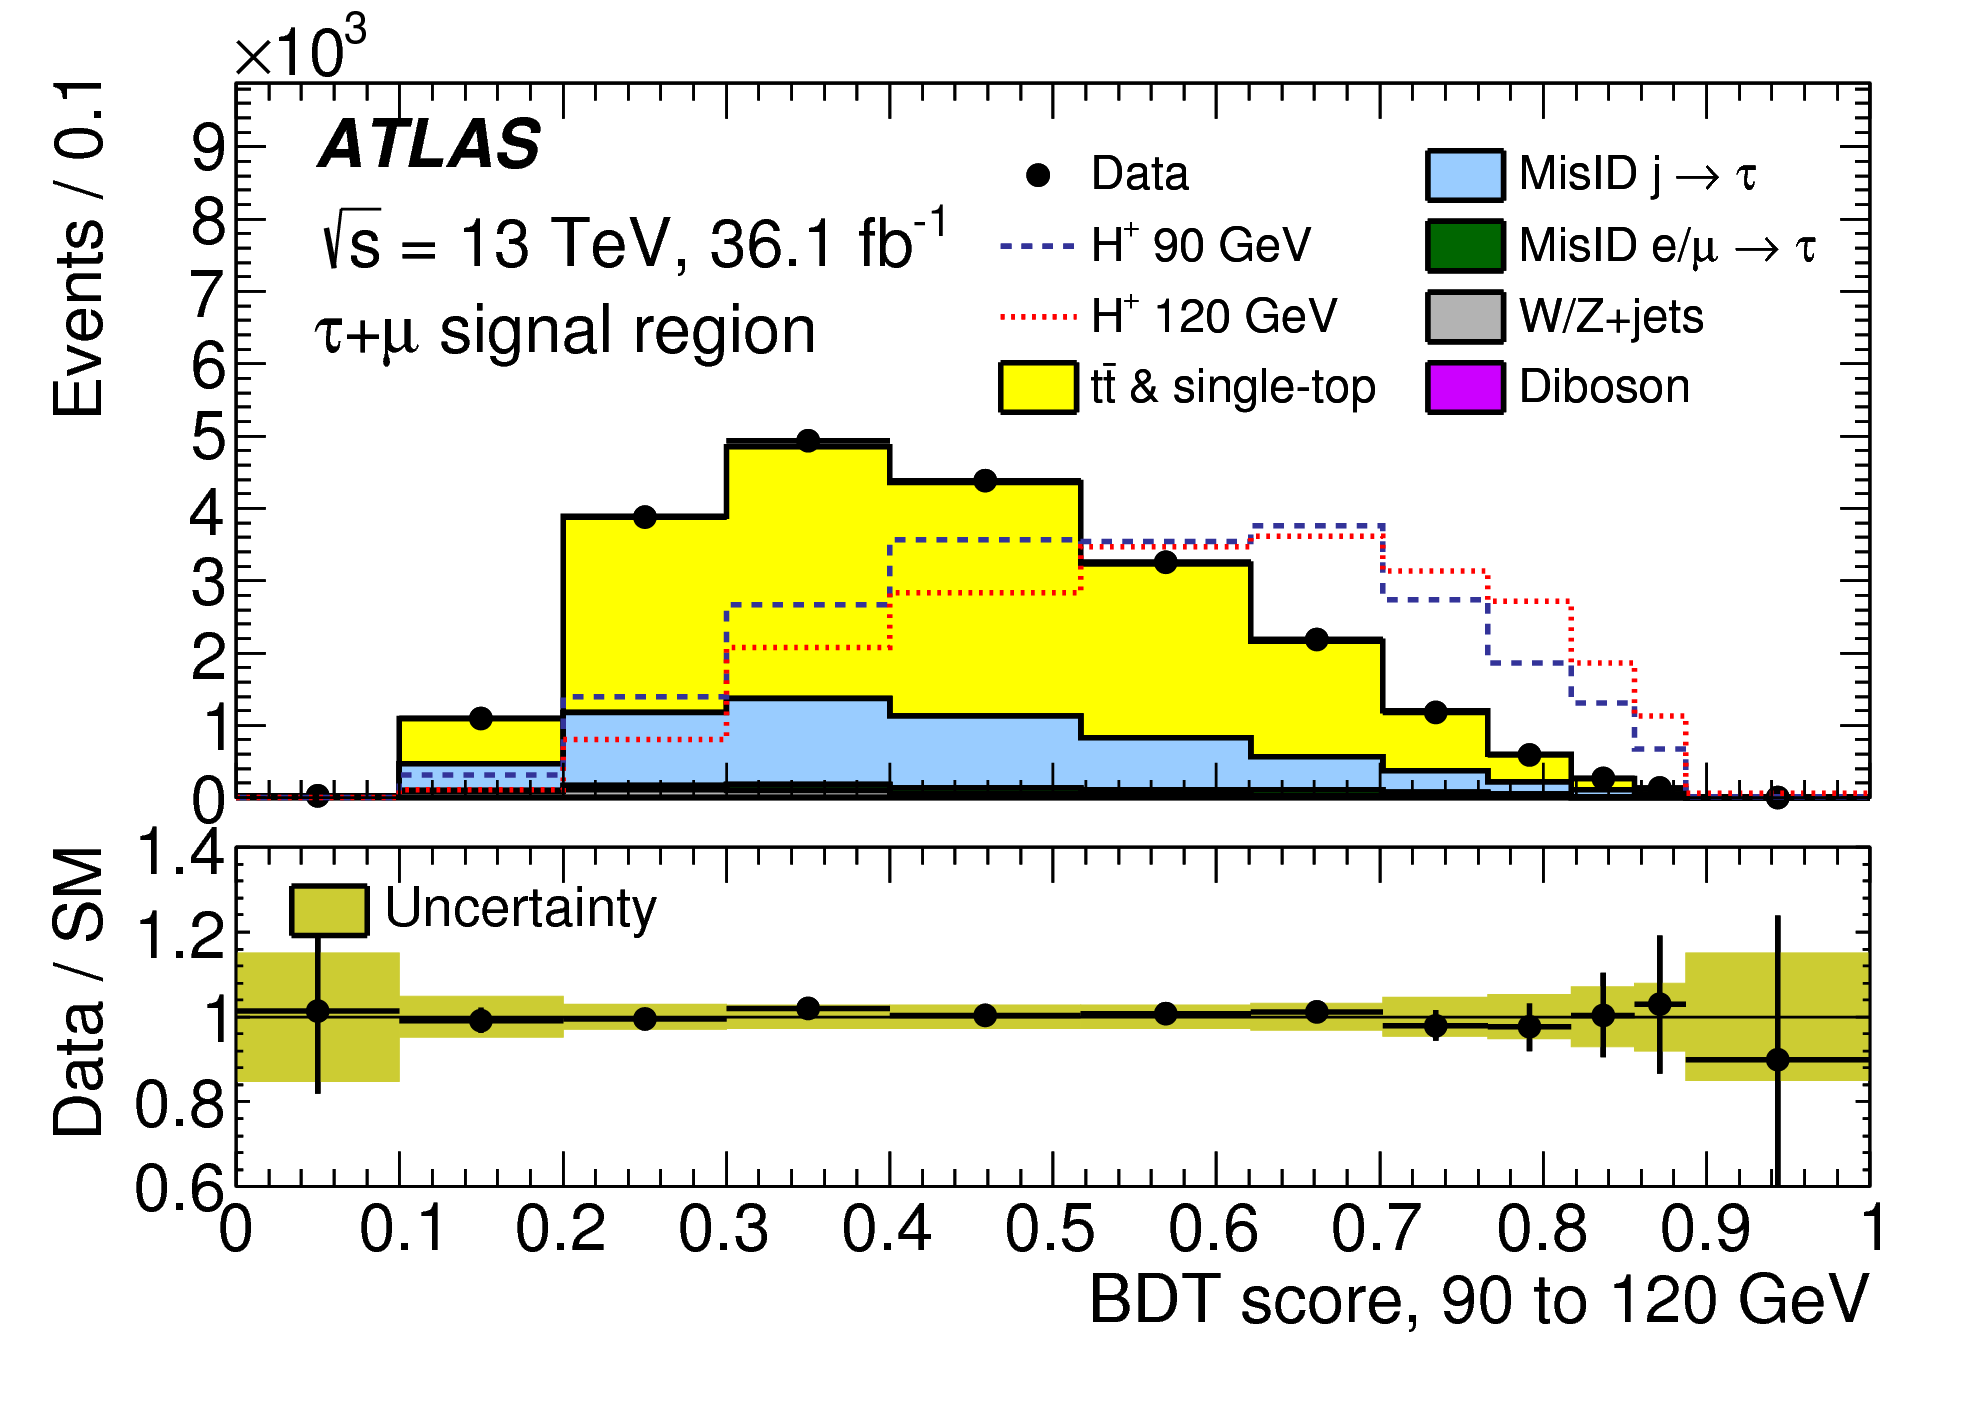
\includegraphics[height=.33\textheight,keepaspectratio=true]{taumu_SR_2018/taumu_SR_90to120_2018.png}

          % \column{.2\textwidth}
          % 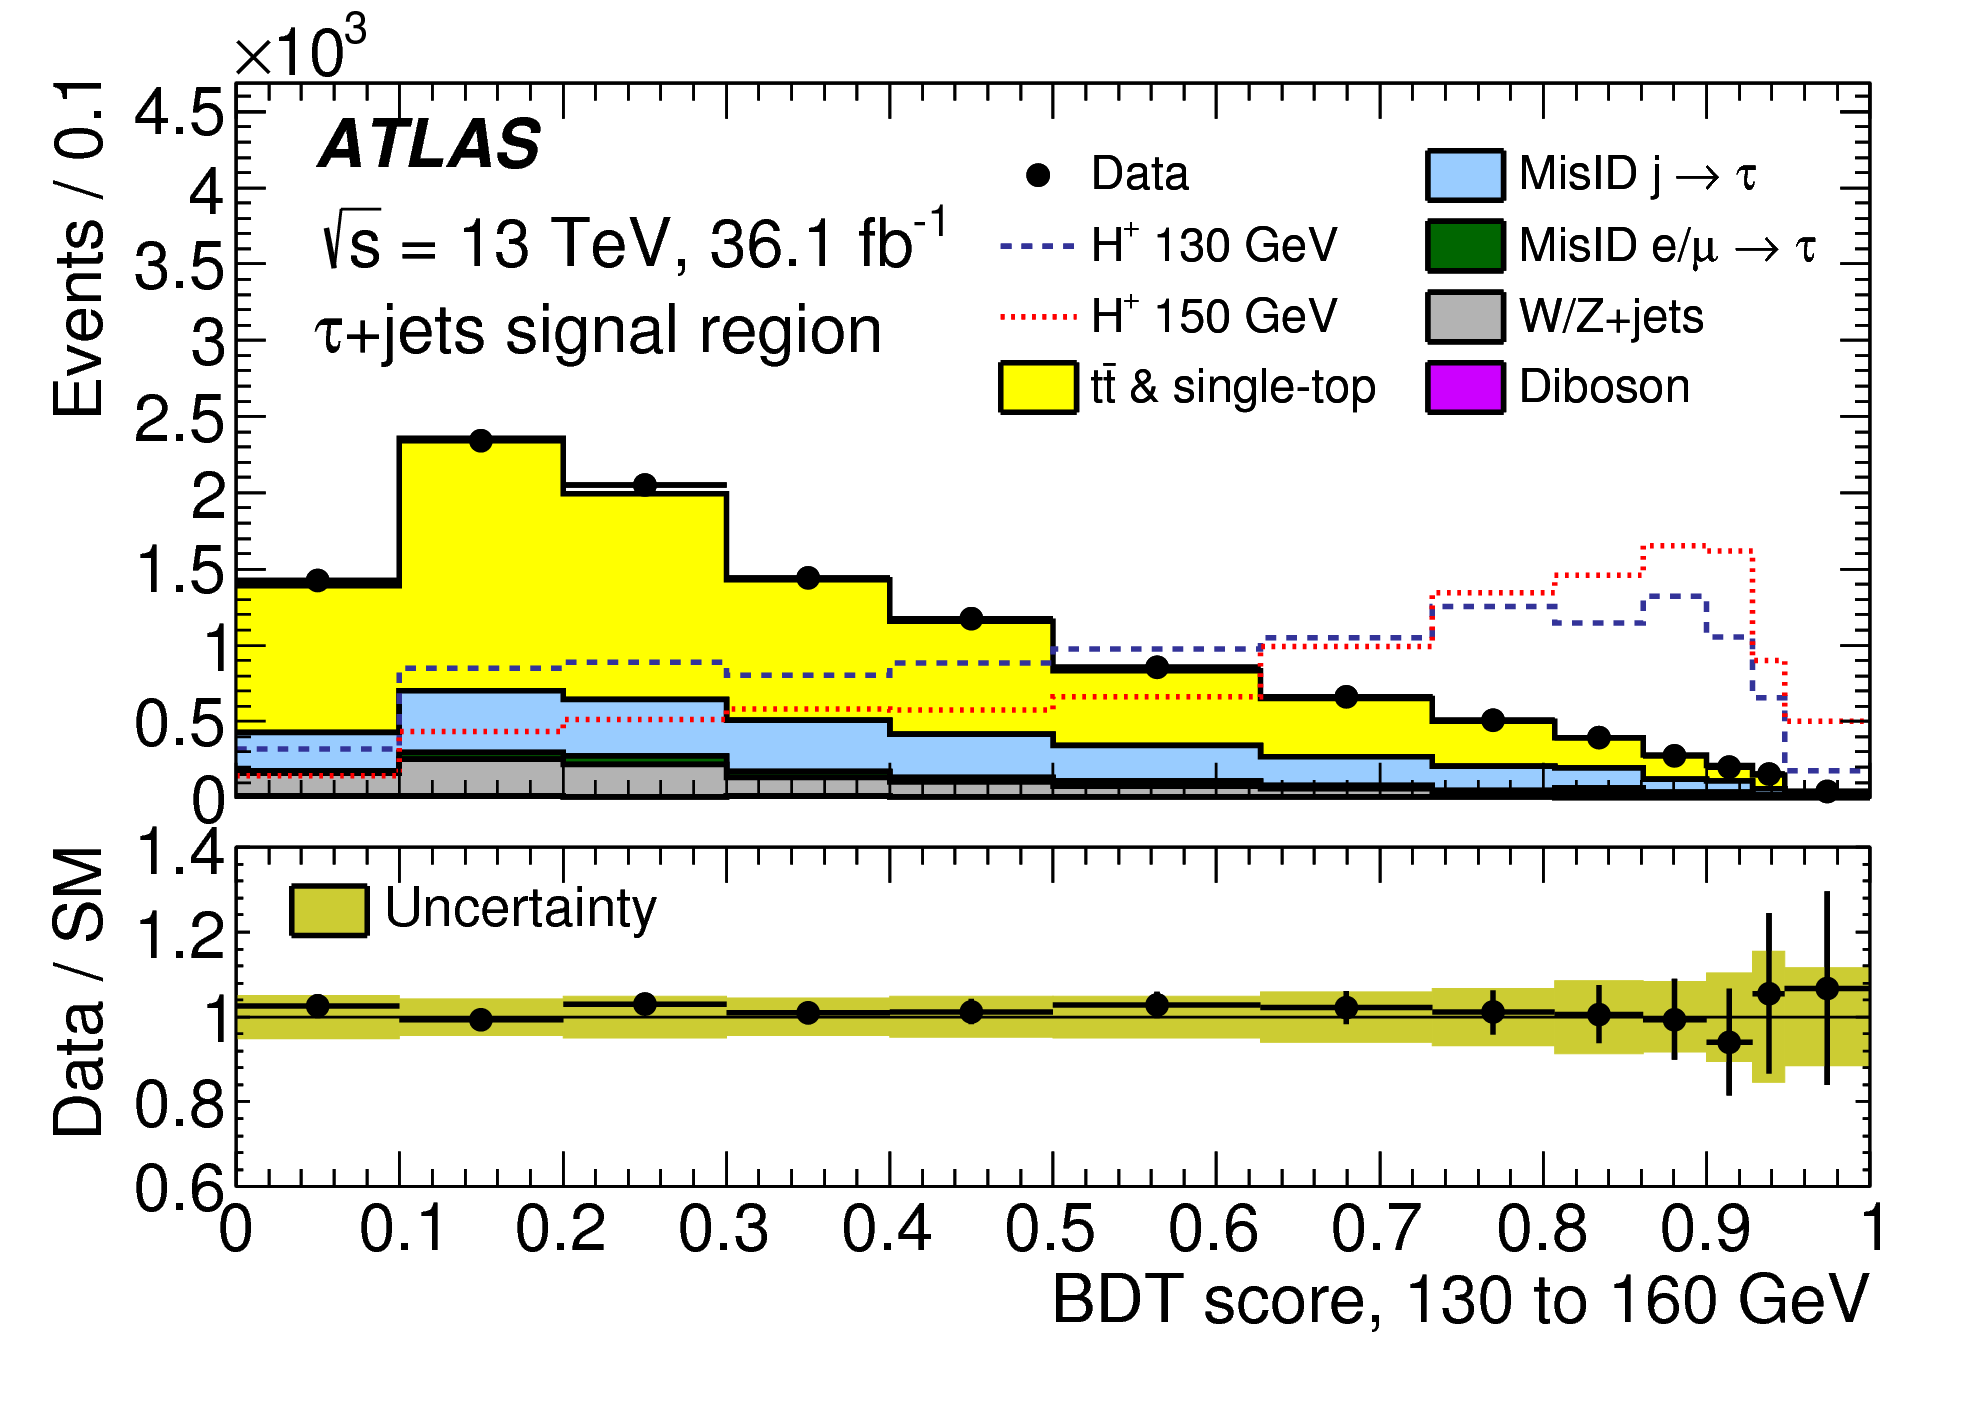
\includegraphics[height=.26\textheight,keepaspectratio=true]{taujet_SR_2018/taujet_SR_130to160_2018.png}
          % 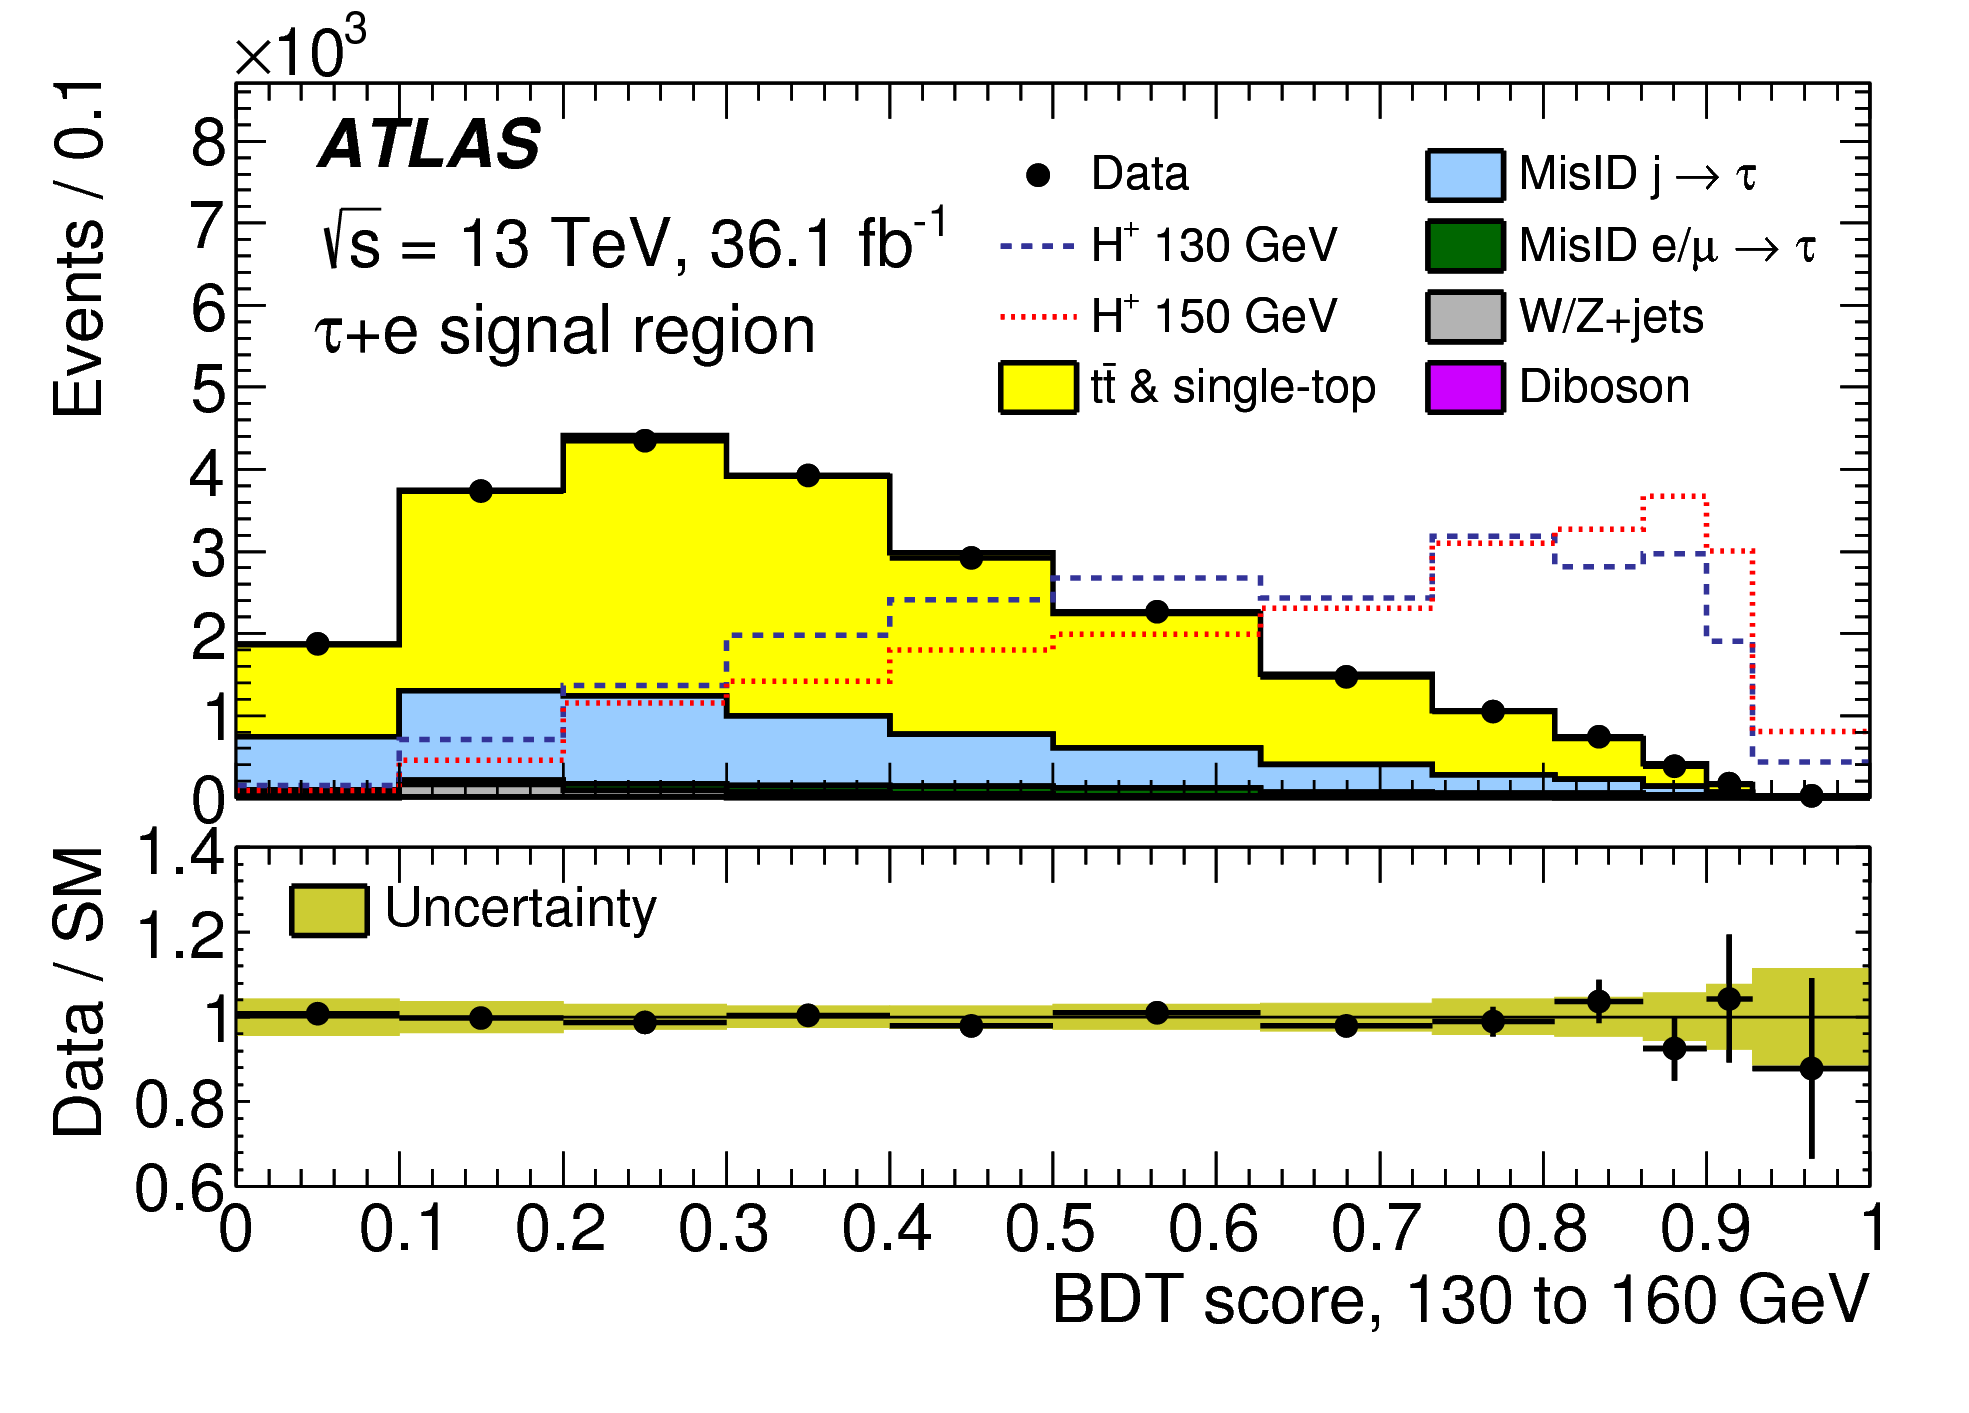
\includegraphics[height=.26\textheight,keepaspectratio=true]{tauel_SR_2018/tauel_SR_130to160_2018.png}
          % 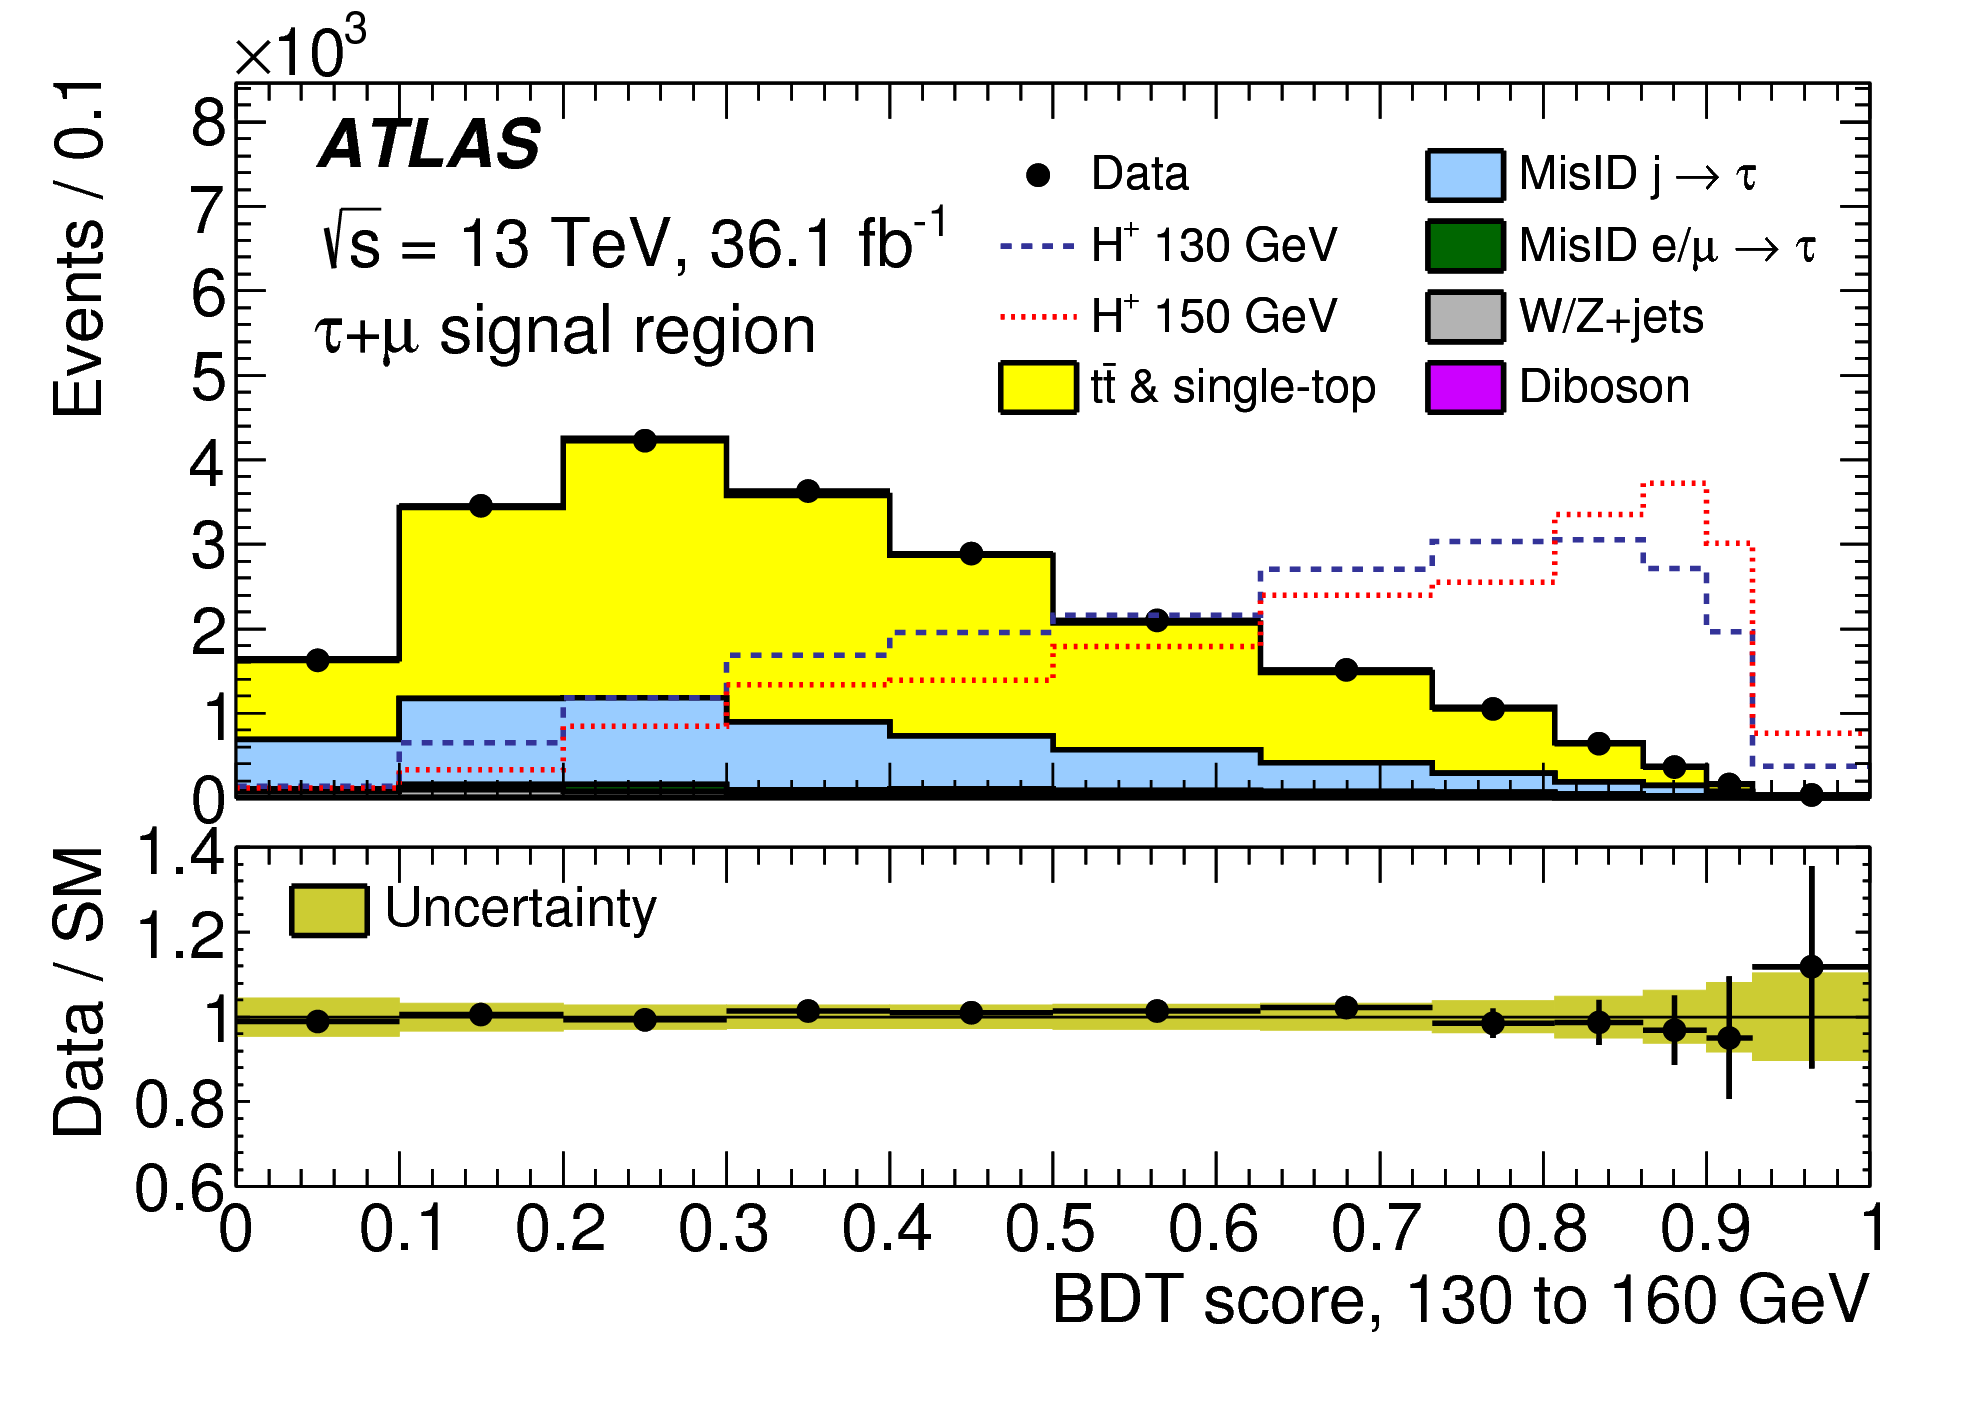
\includegraphics[height=.26\textheight,keepaspectratio=true]{taumu_SR_2018/taumu_SR_130to160_2018.png}

          \column{.33\textwidth}
          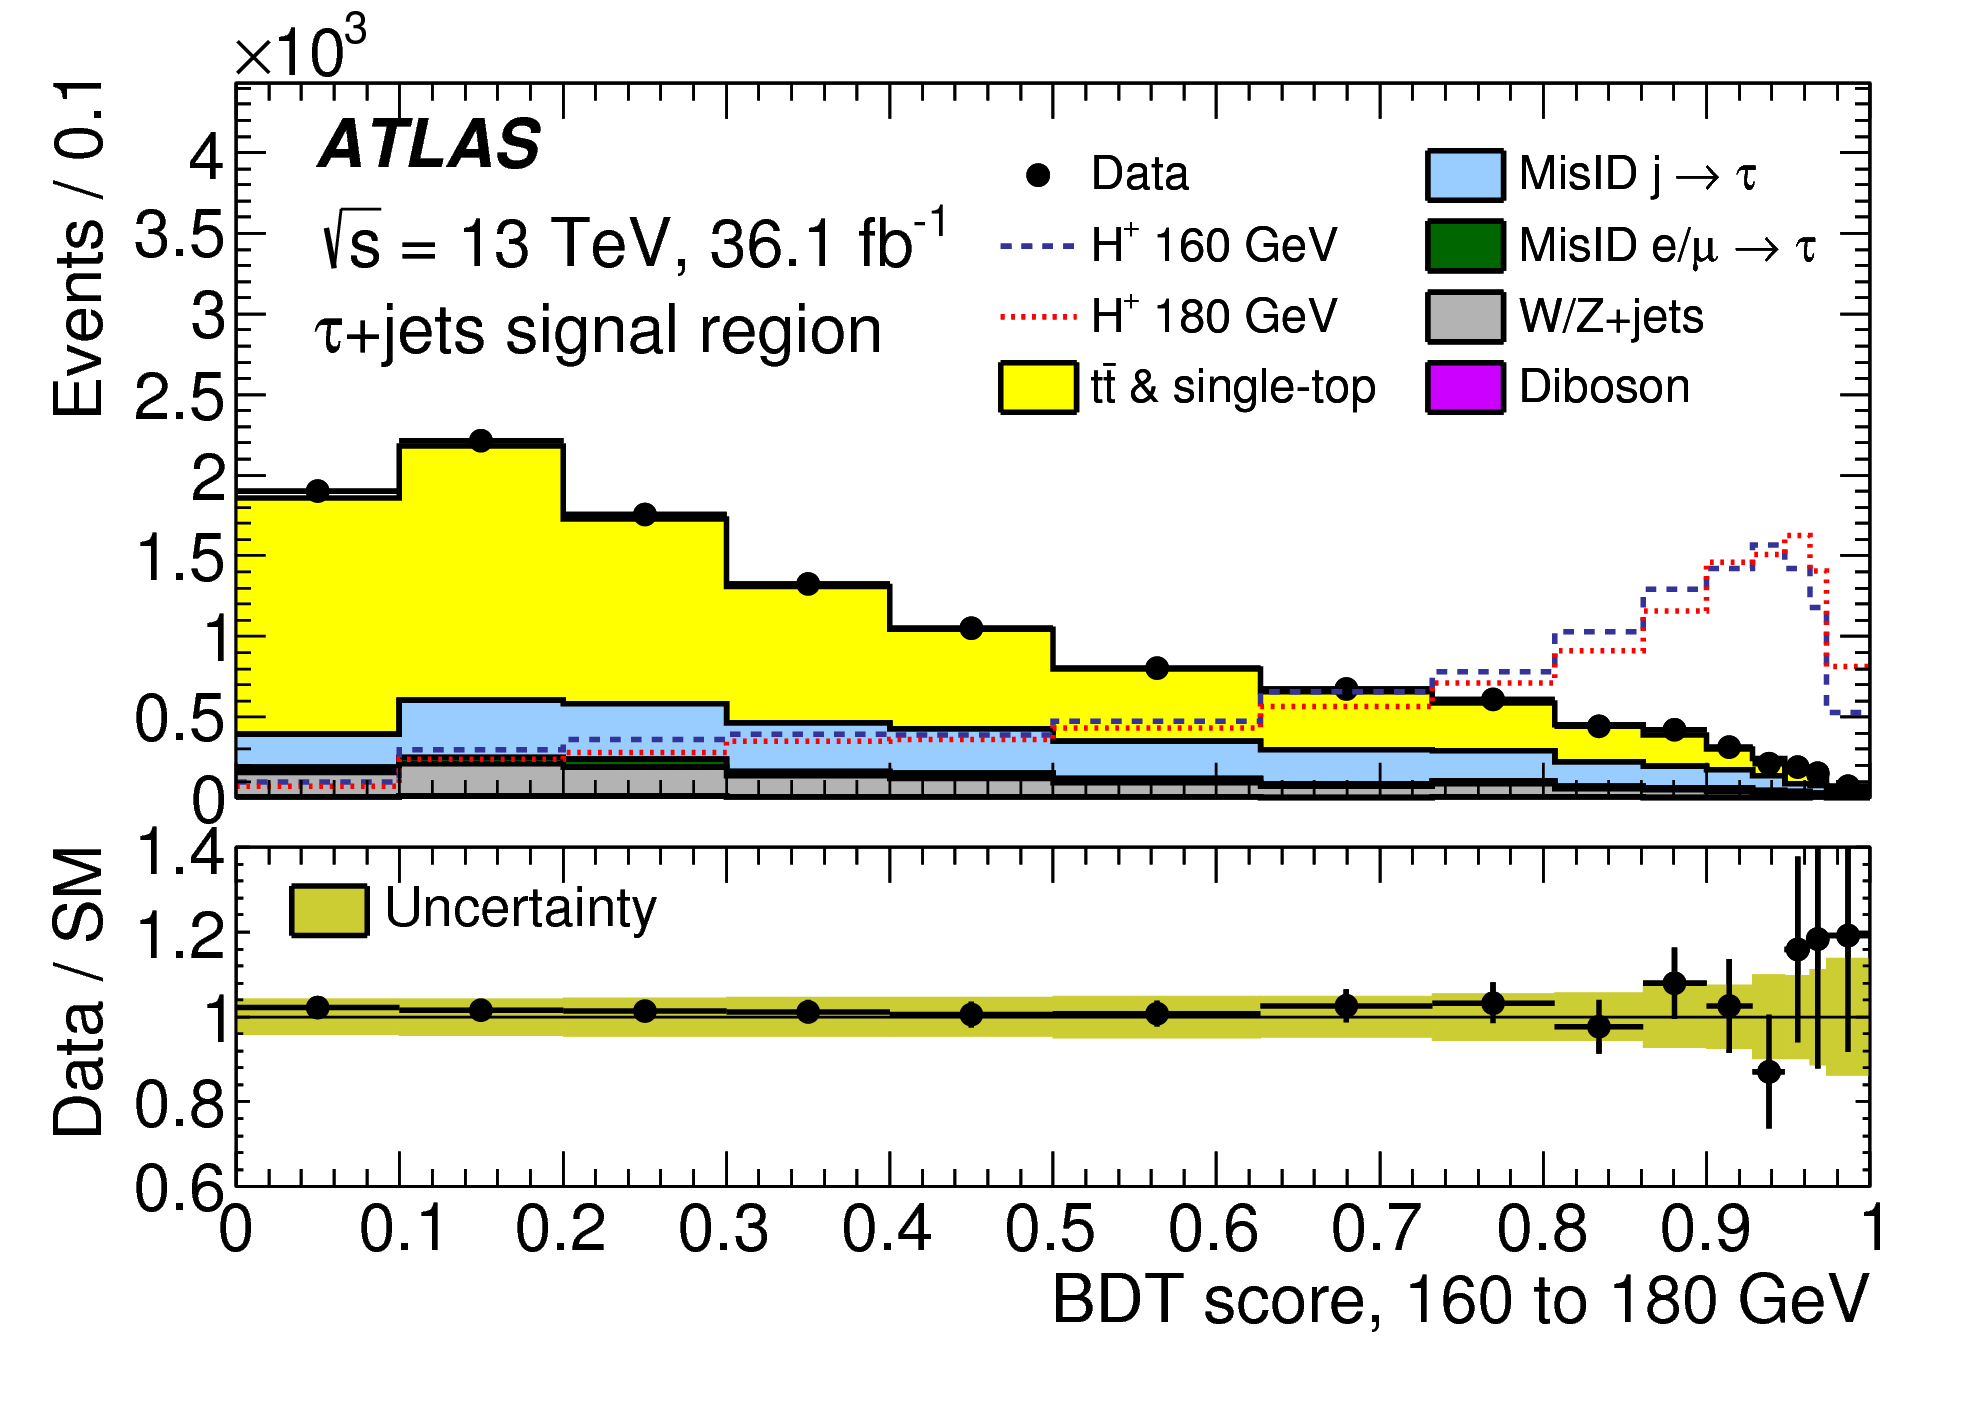
\includegraphics[height=.4\textheight,keepaspectratio=true]{taujet_SR_2018/taujet_SR_160to180_2018.png}
          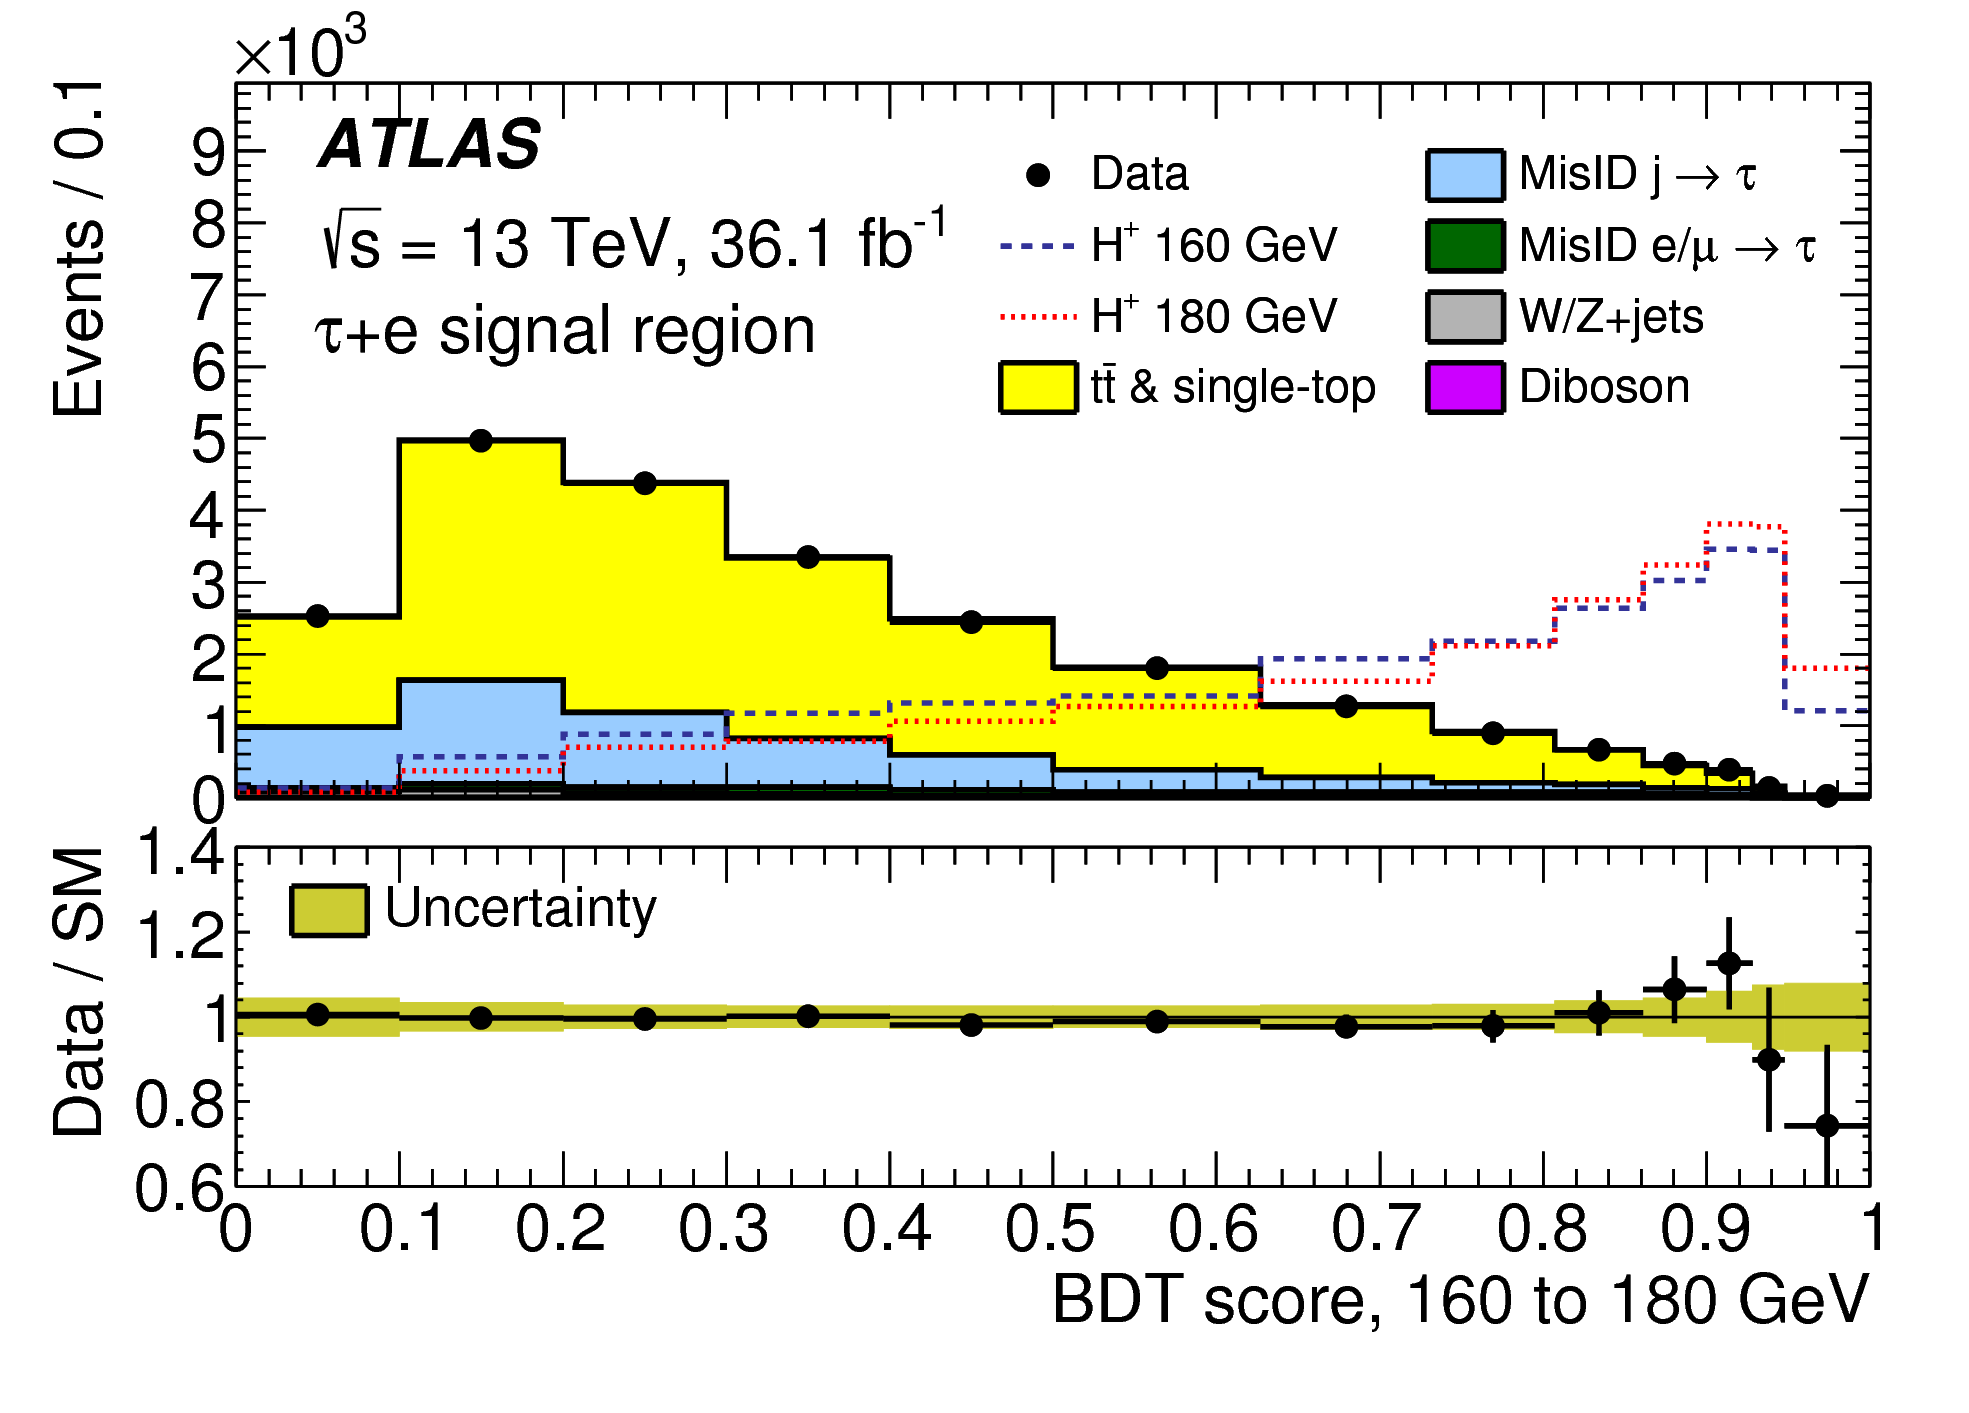
\includegraphics[height=.4\textheight,keepaspectratio=true]{tauel_SR_2018/tauel_SR_160to180_2018.png}
          % 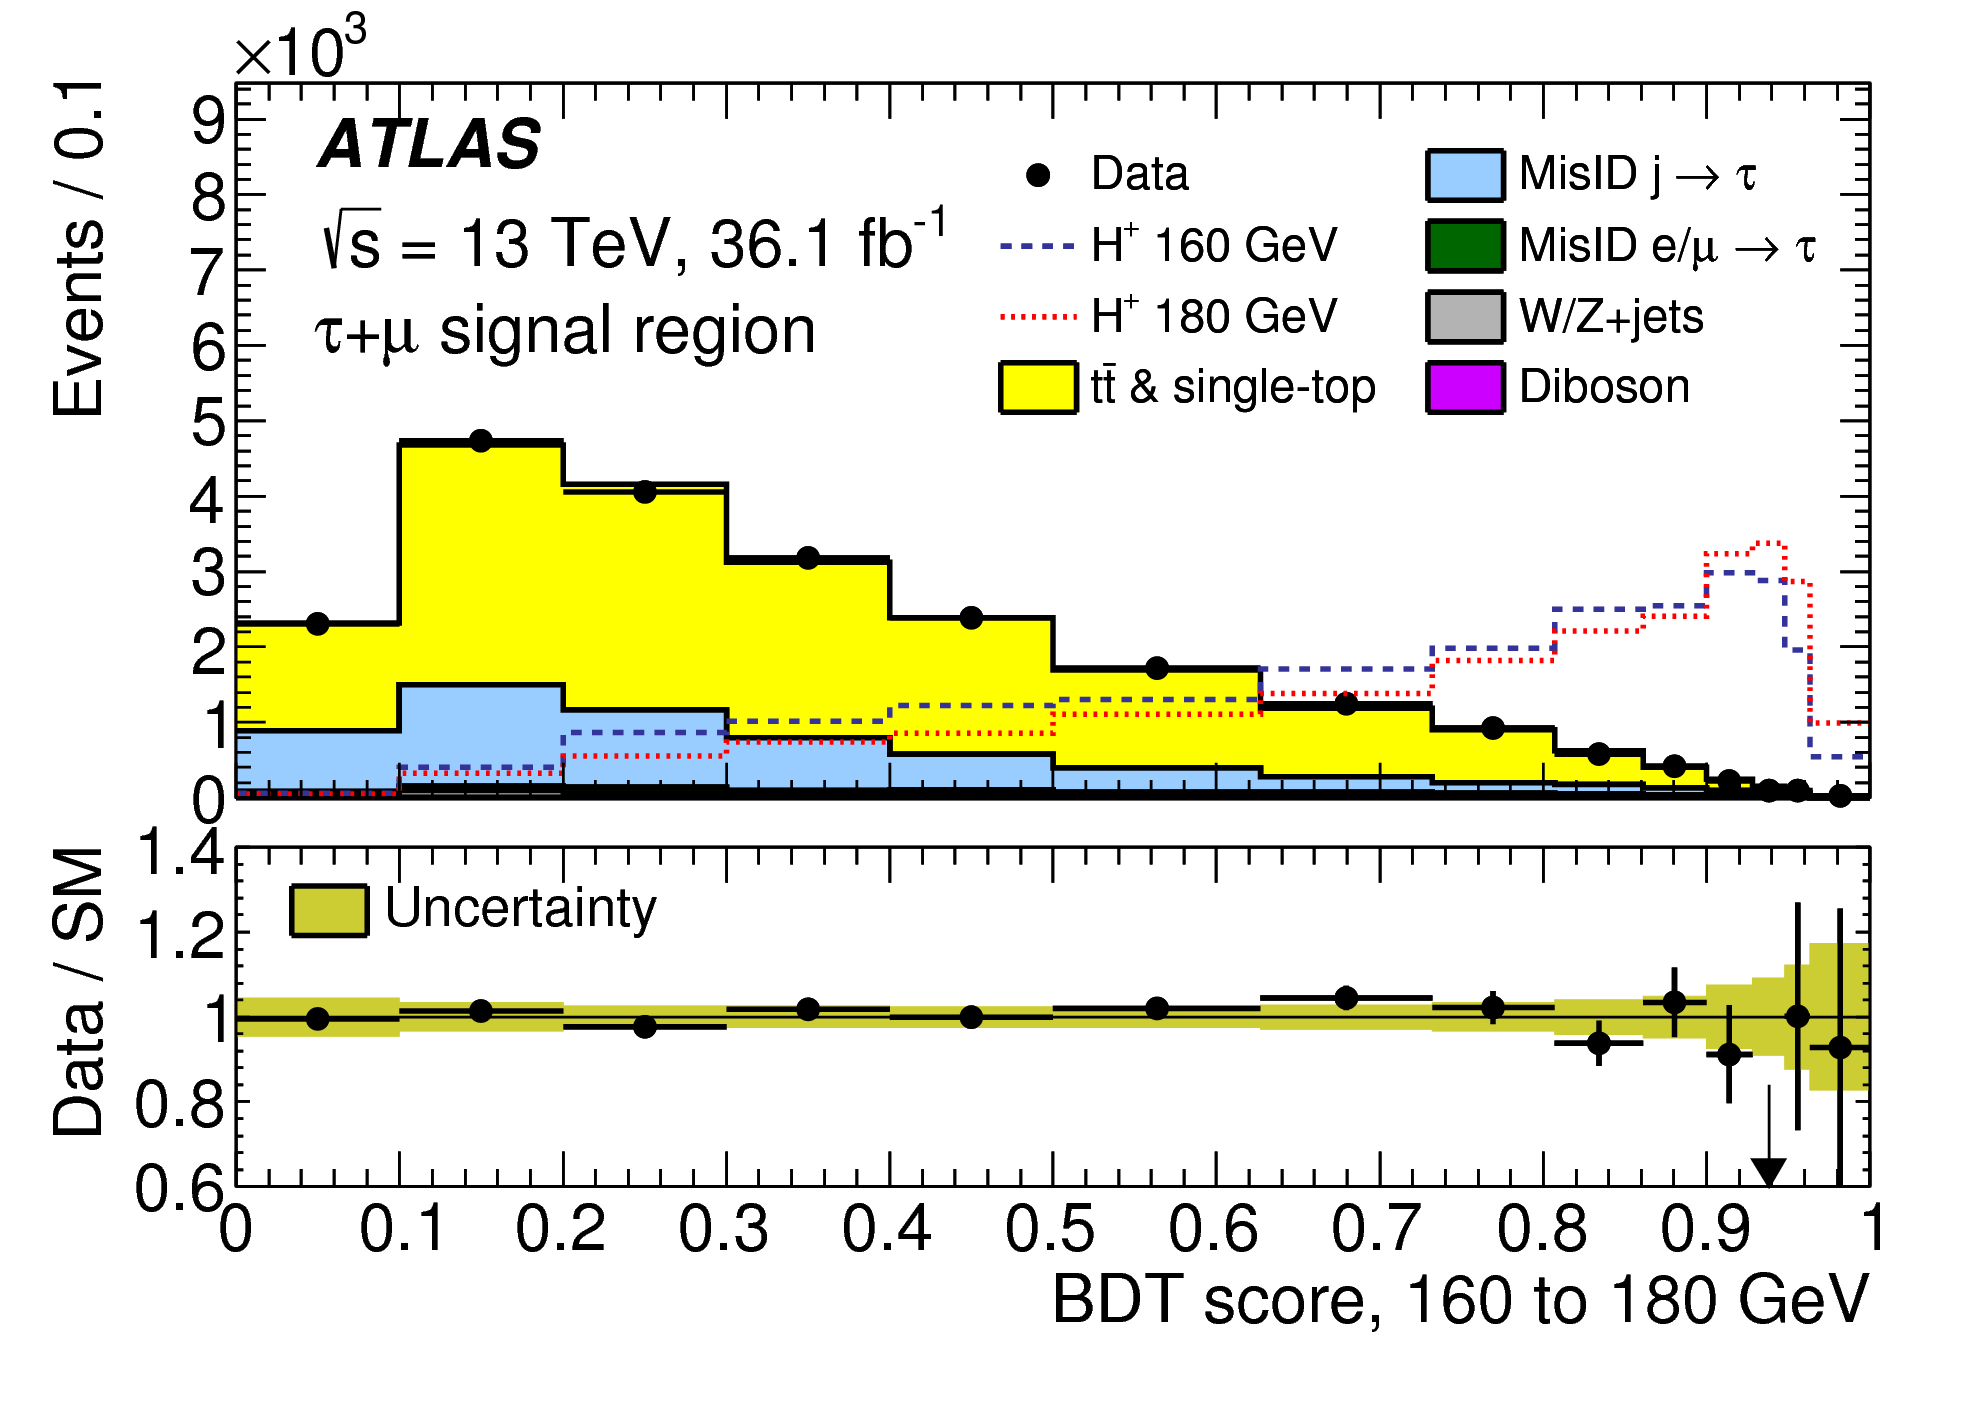
\includegraphics[height=.33\textheight,keepaspectratio=true]{taumu_SR_2018/taumu_SR_160to180_2018.png}


          \column{.33\textwidth}
          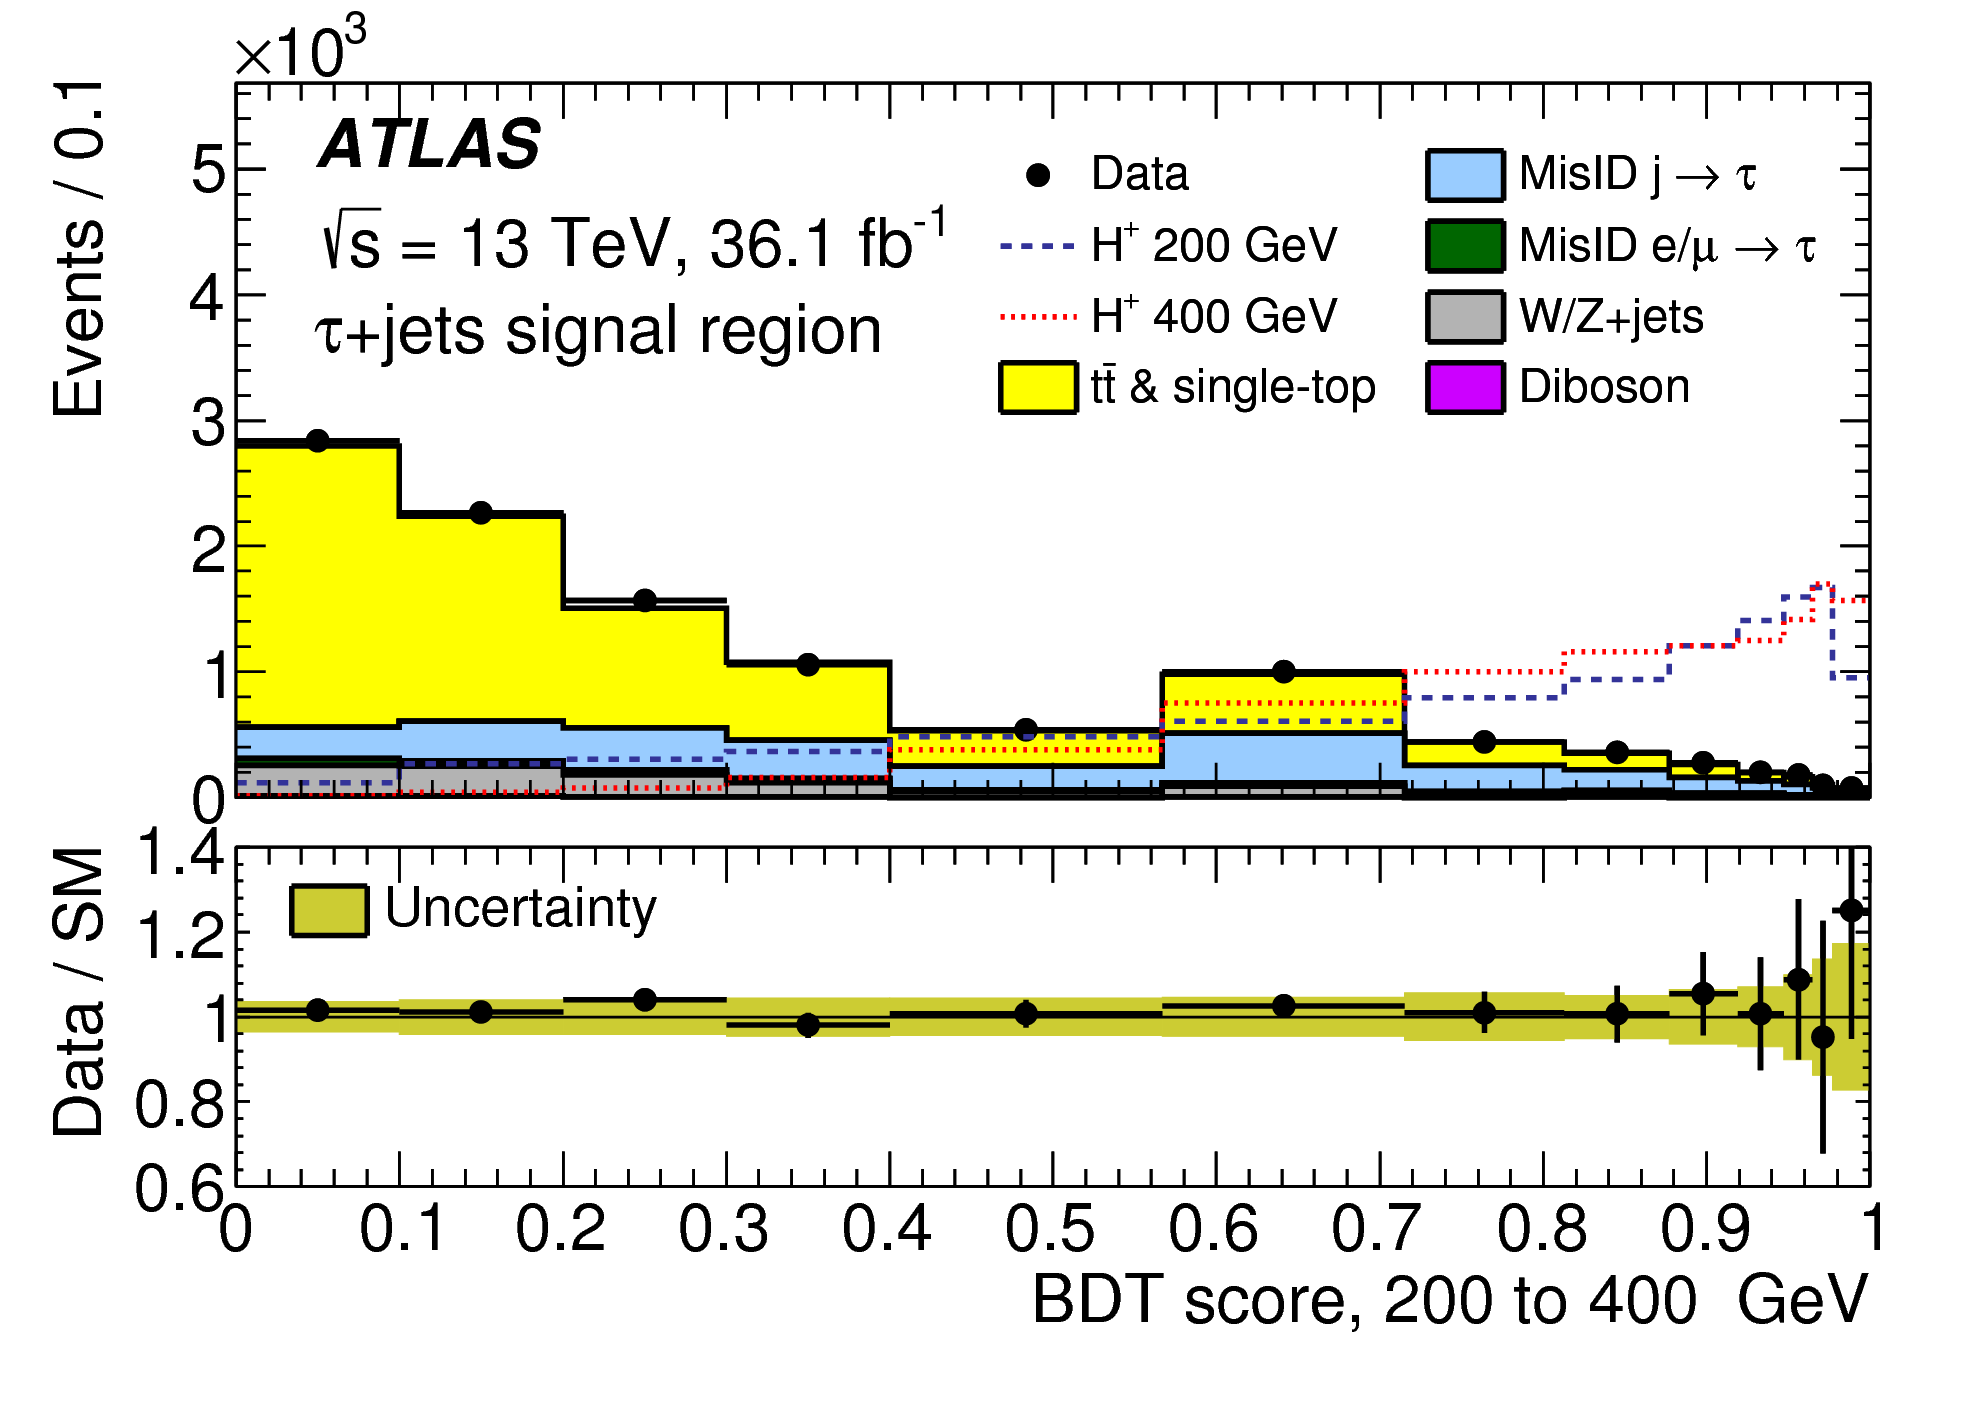
\includegraphics[height=.4\textheight,keepaspectratio=true]{taujet_SR_2018/taujet_SR_200to400_2018.png}
          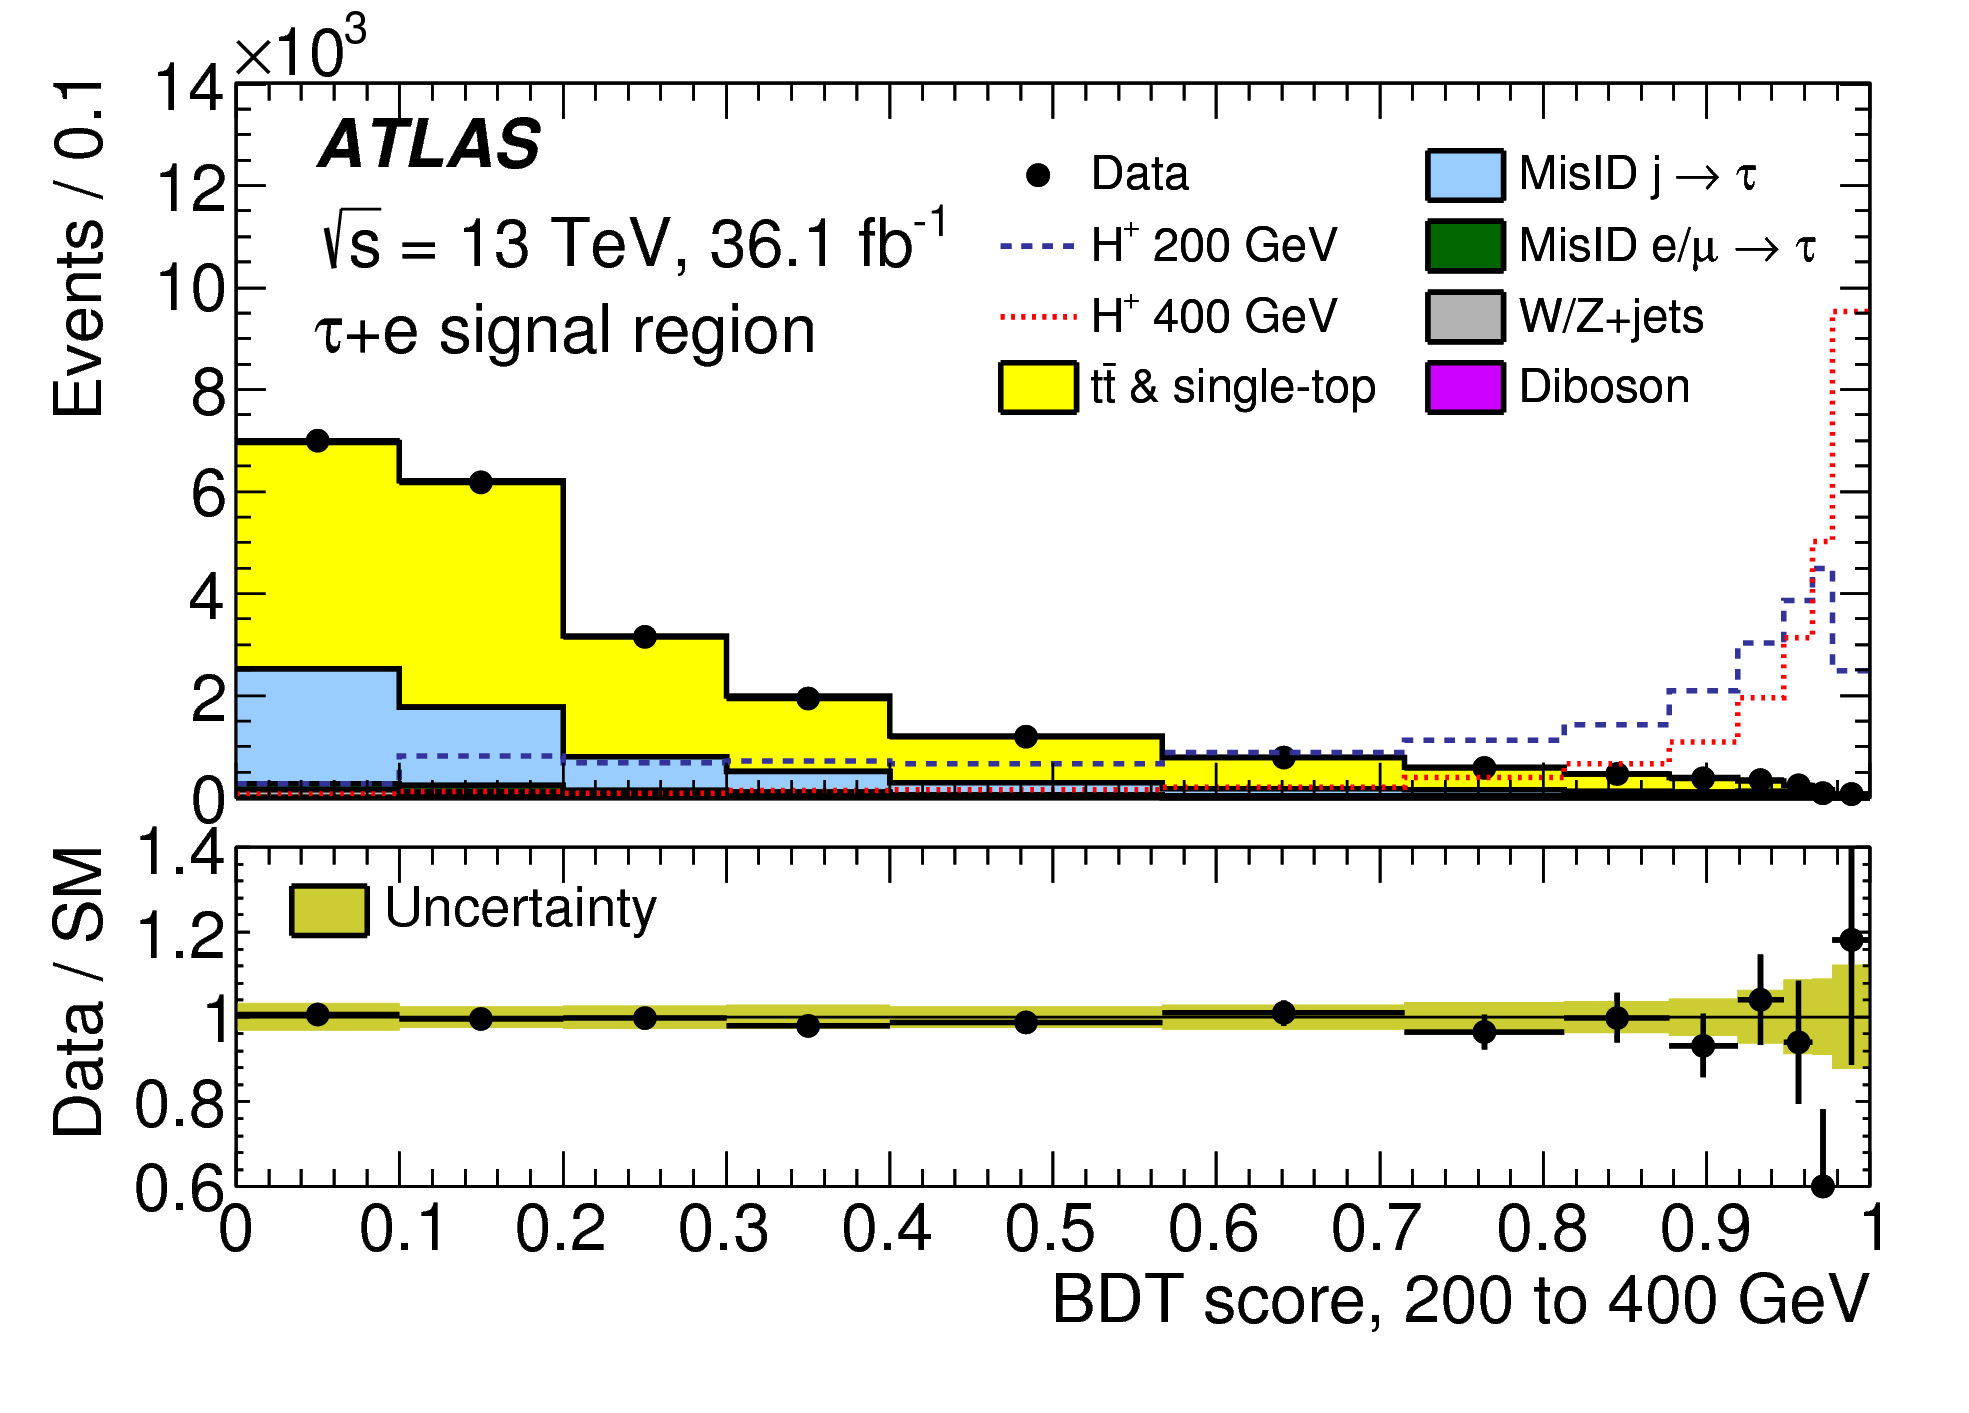
\includegraphics[height=.4\textheight,keepaspectratio=true]{tauel_SR_2018/tauel_SR_200to400_2018.png}
          % 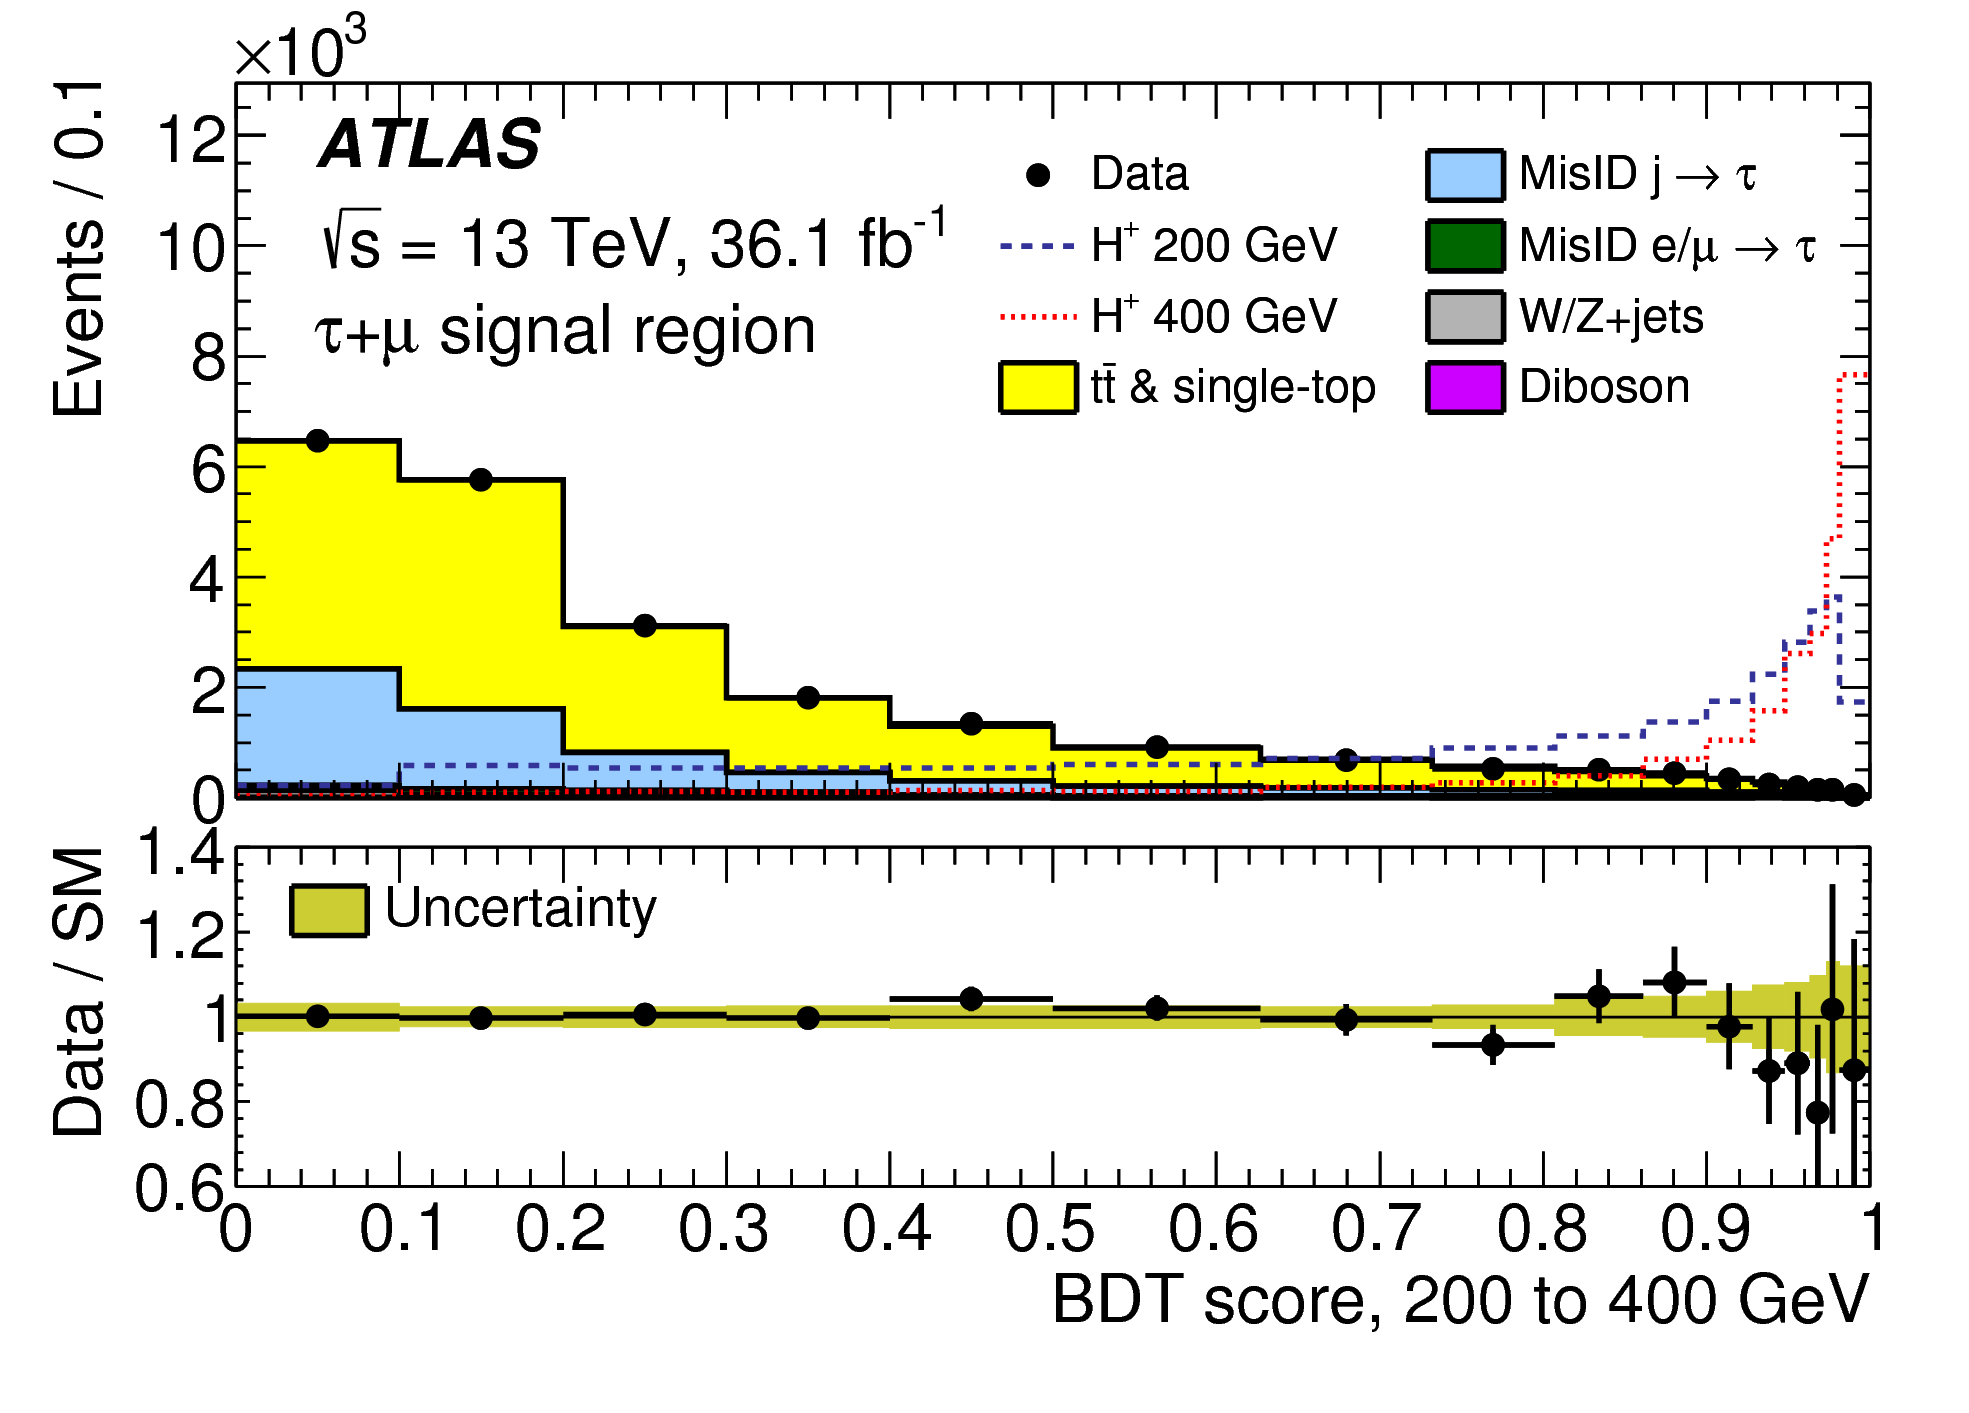
\includegraphics[height=.33\textheight,keepaspectratio=true]{taumu_SR_2018/taumu_SR_200to400_2018.png}


          % \column{.2\textwidth}
          % 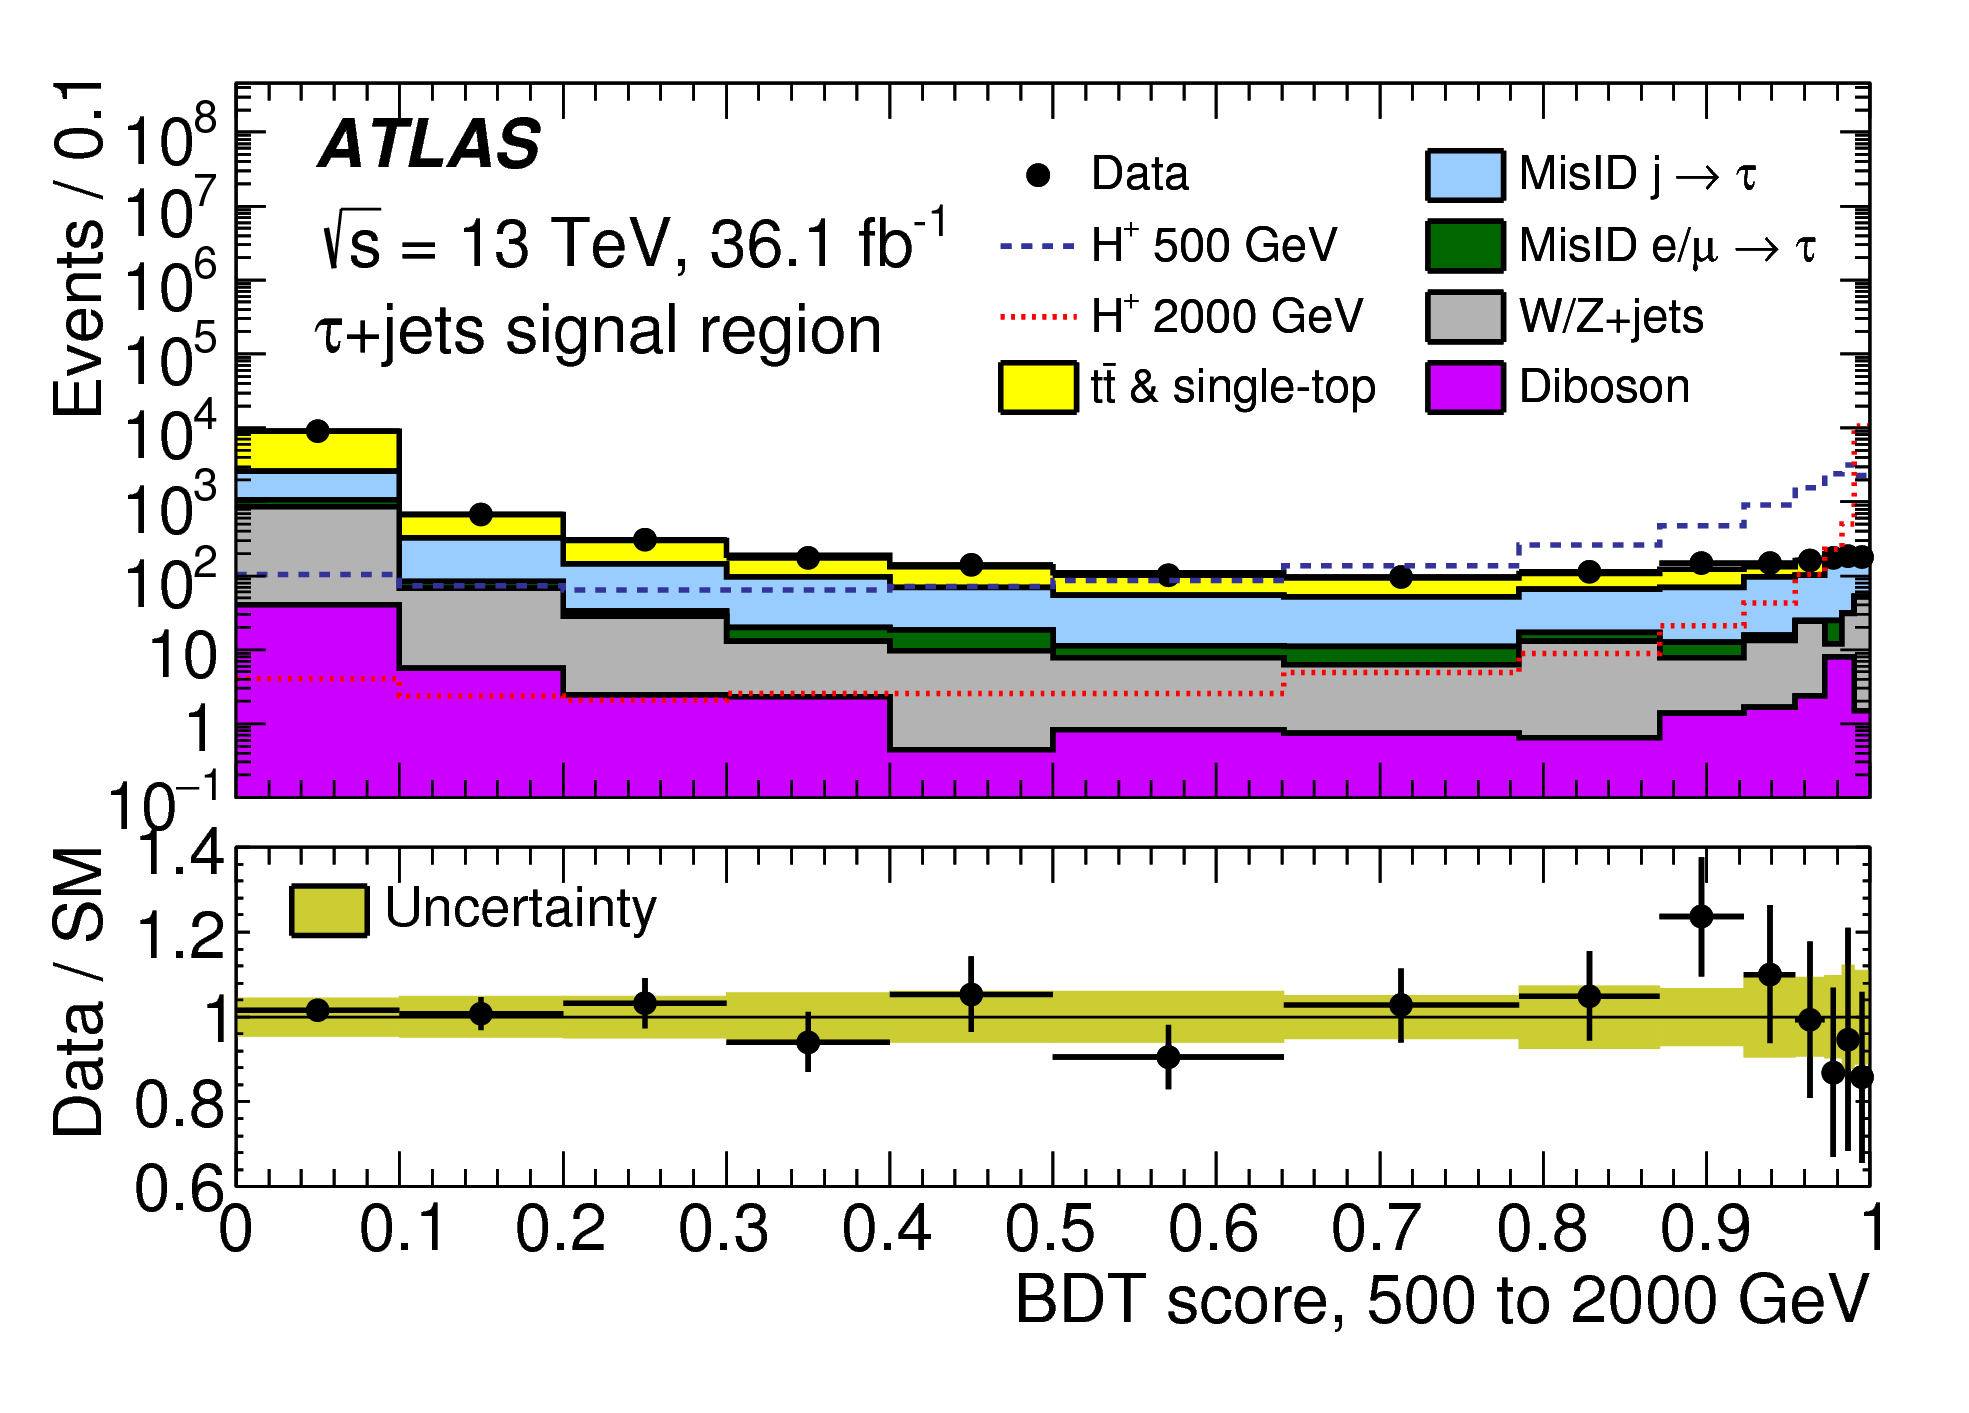
\includegraphics[height=.26\textheight,keepaspectratio=true]{taujet_SR_2018/taujet_SR_500to2000_2018.png}
          % 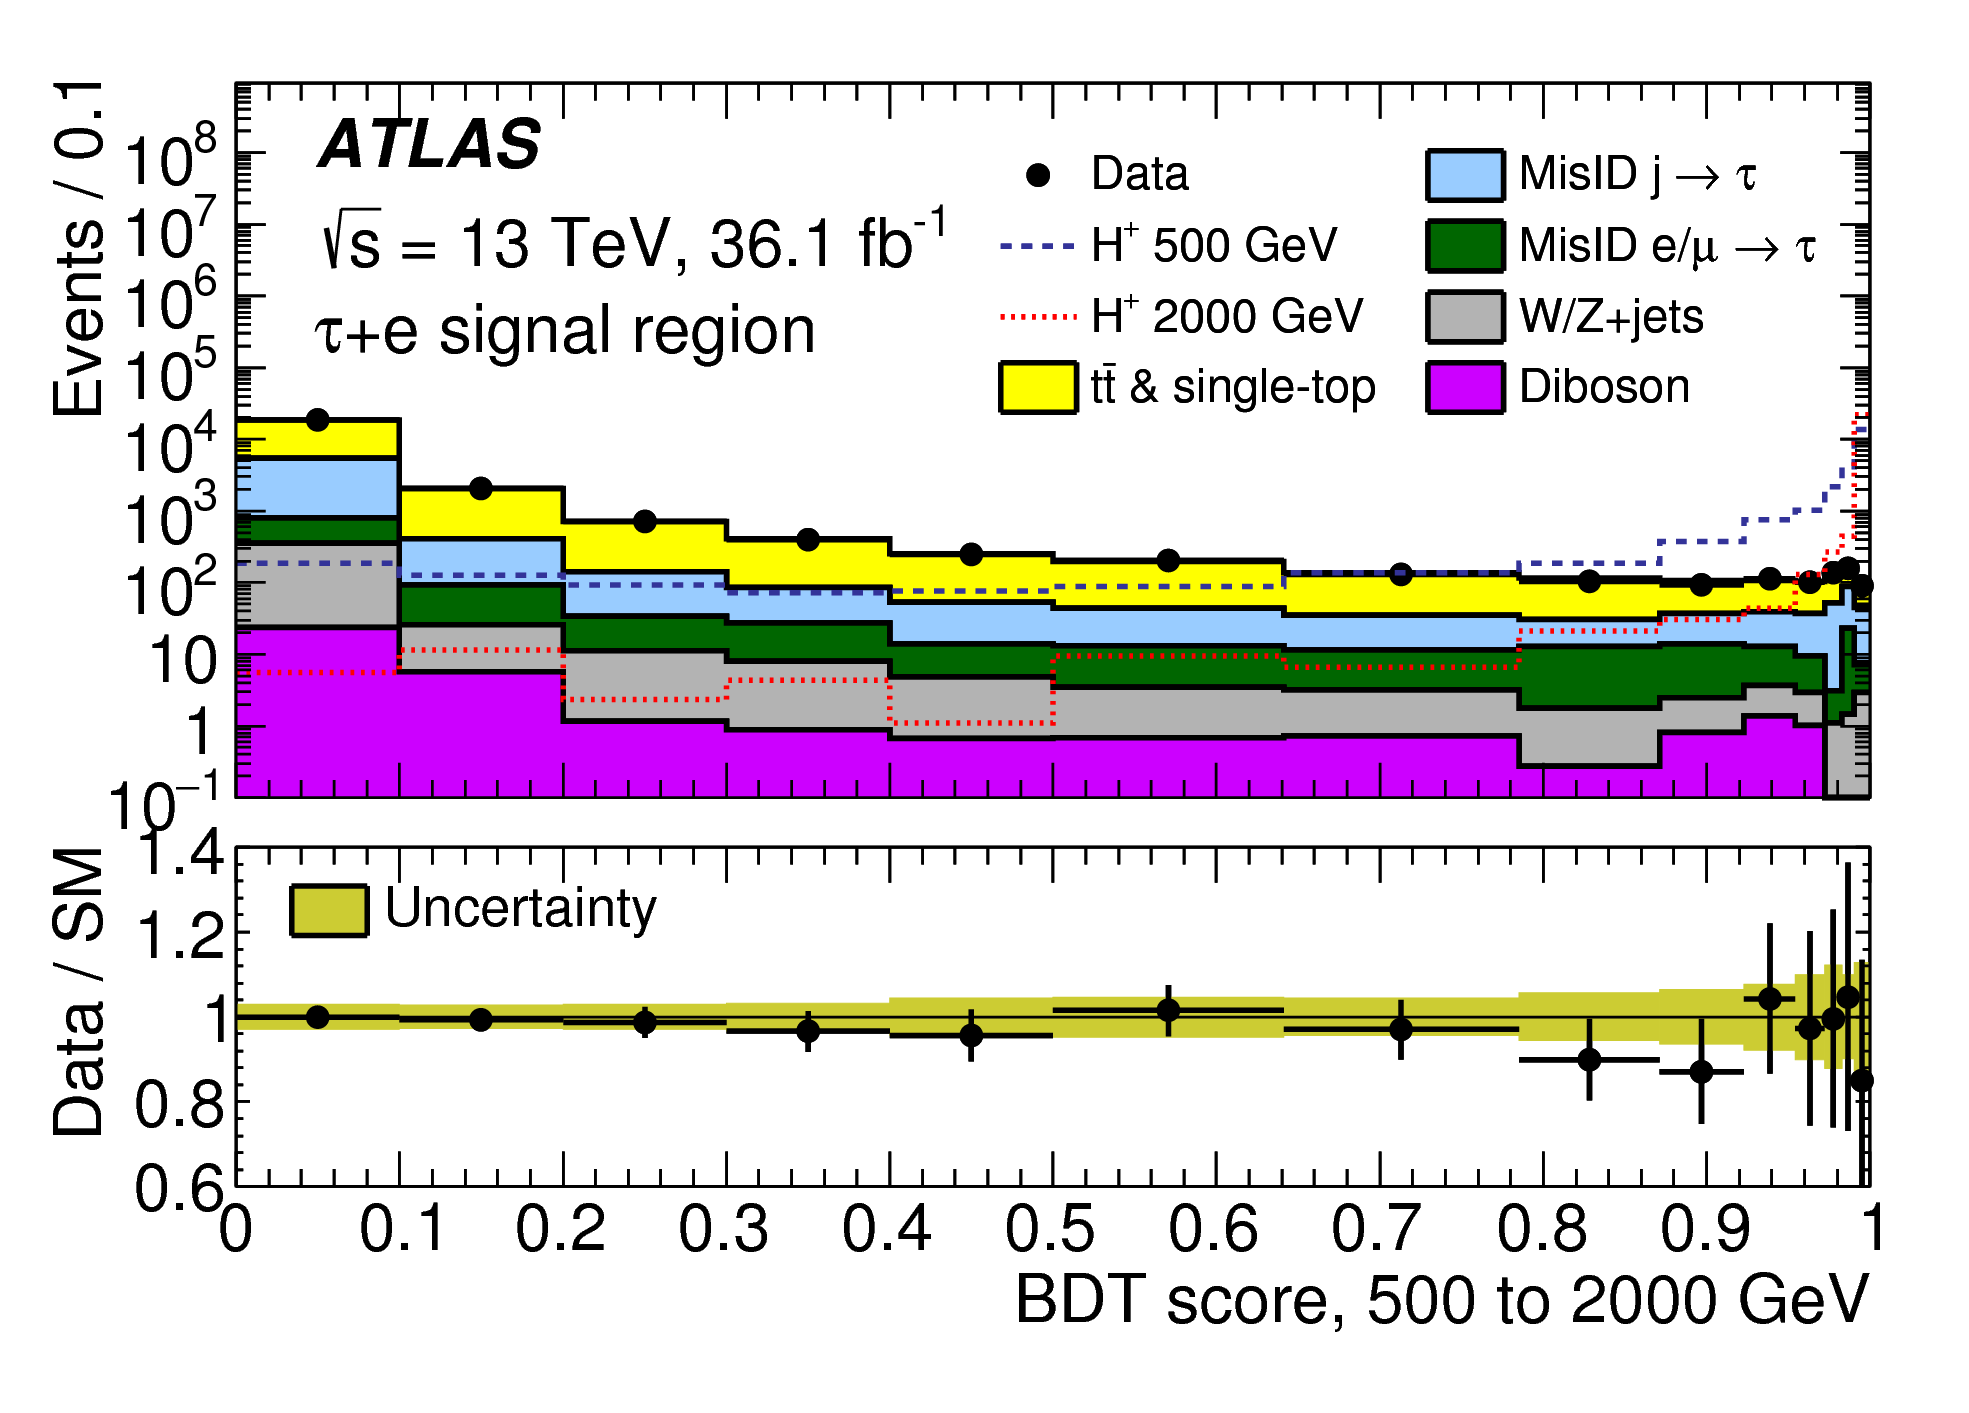
\includegraphics[height=.26\textheight,keepaspectratio=true]{tauel_SR_2018/tauel_SR_500to2000_2018.png}
          % 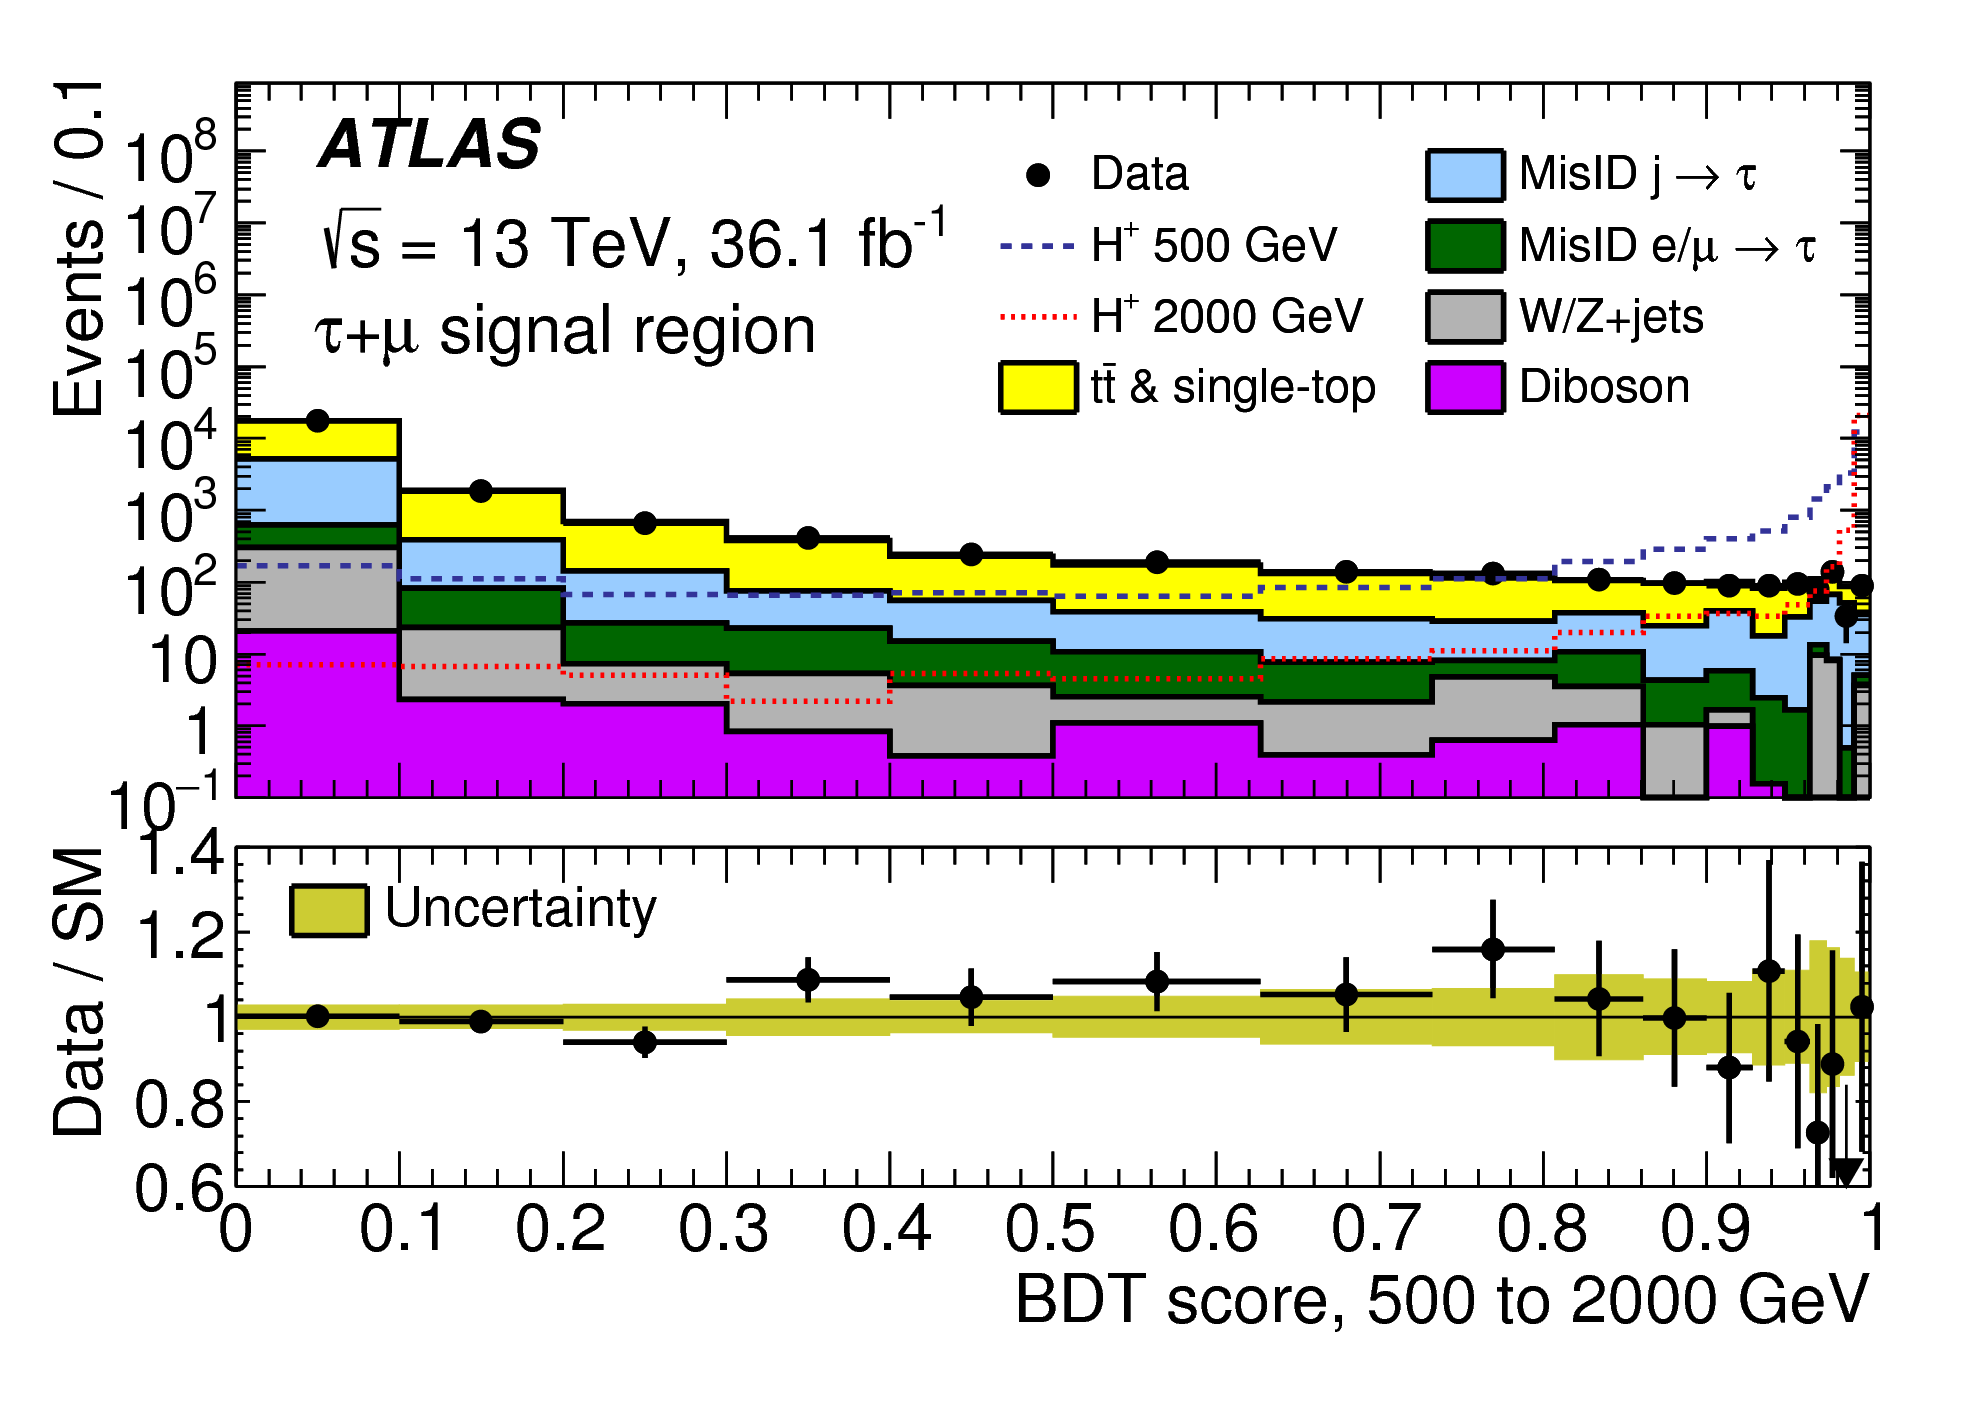
\includegraphics[height=.26\textheight,keepaspectratio=true]{taumu_SR_2018/taumu_SR_500to2000_2018.png}
        \end{columns}
      \end{frame}

    \begin{frame}{\href{https://link.springer.com/article/10.1007/JHEP09(2018)139}{\textcolor{blue}{JHEP 09(2018)139}} Limits}
      \begin{columns}
        \column{.5\textwidth}
        \centering
        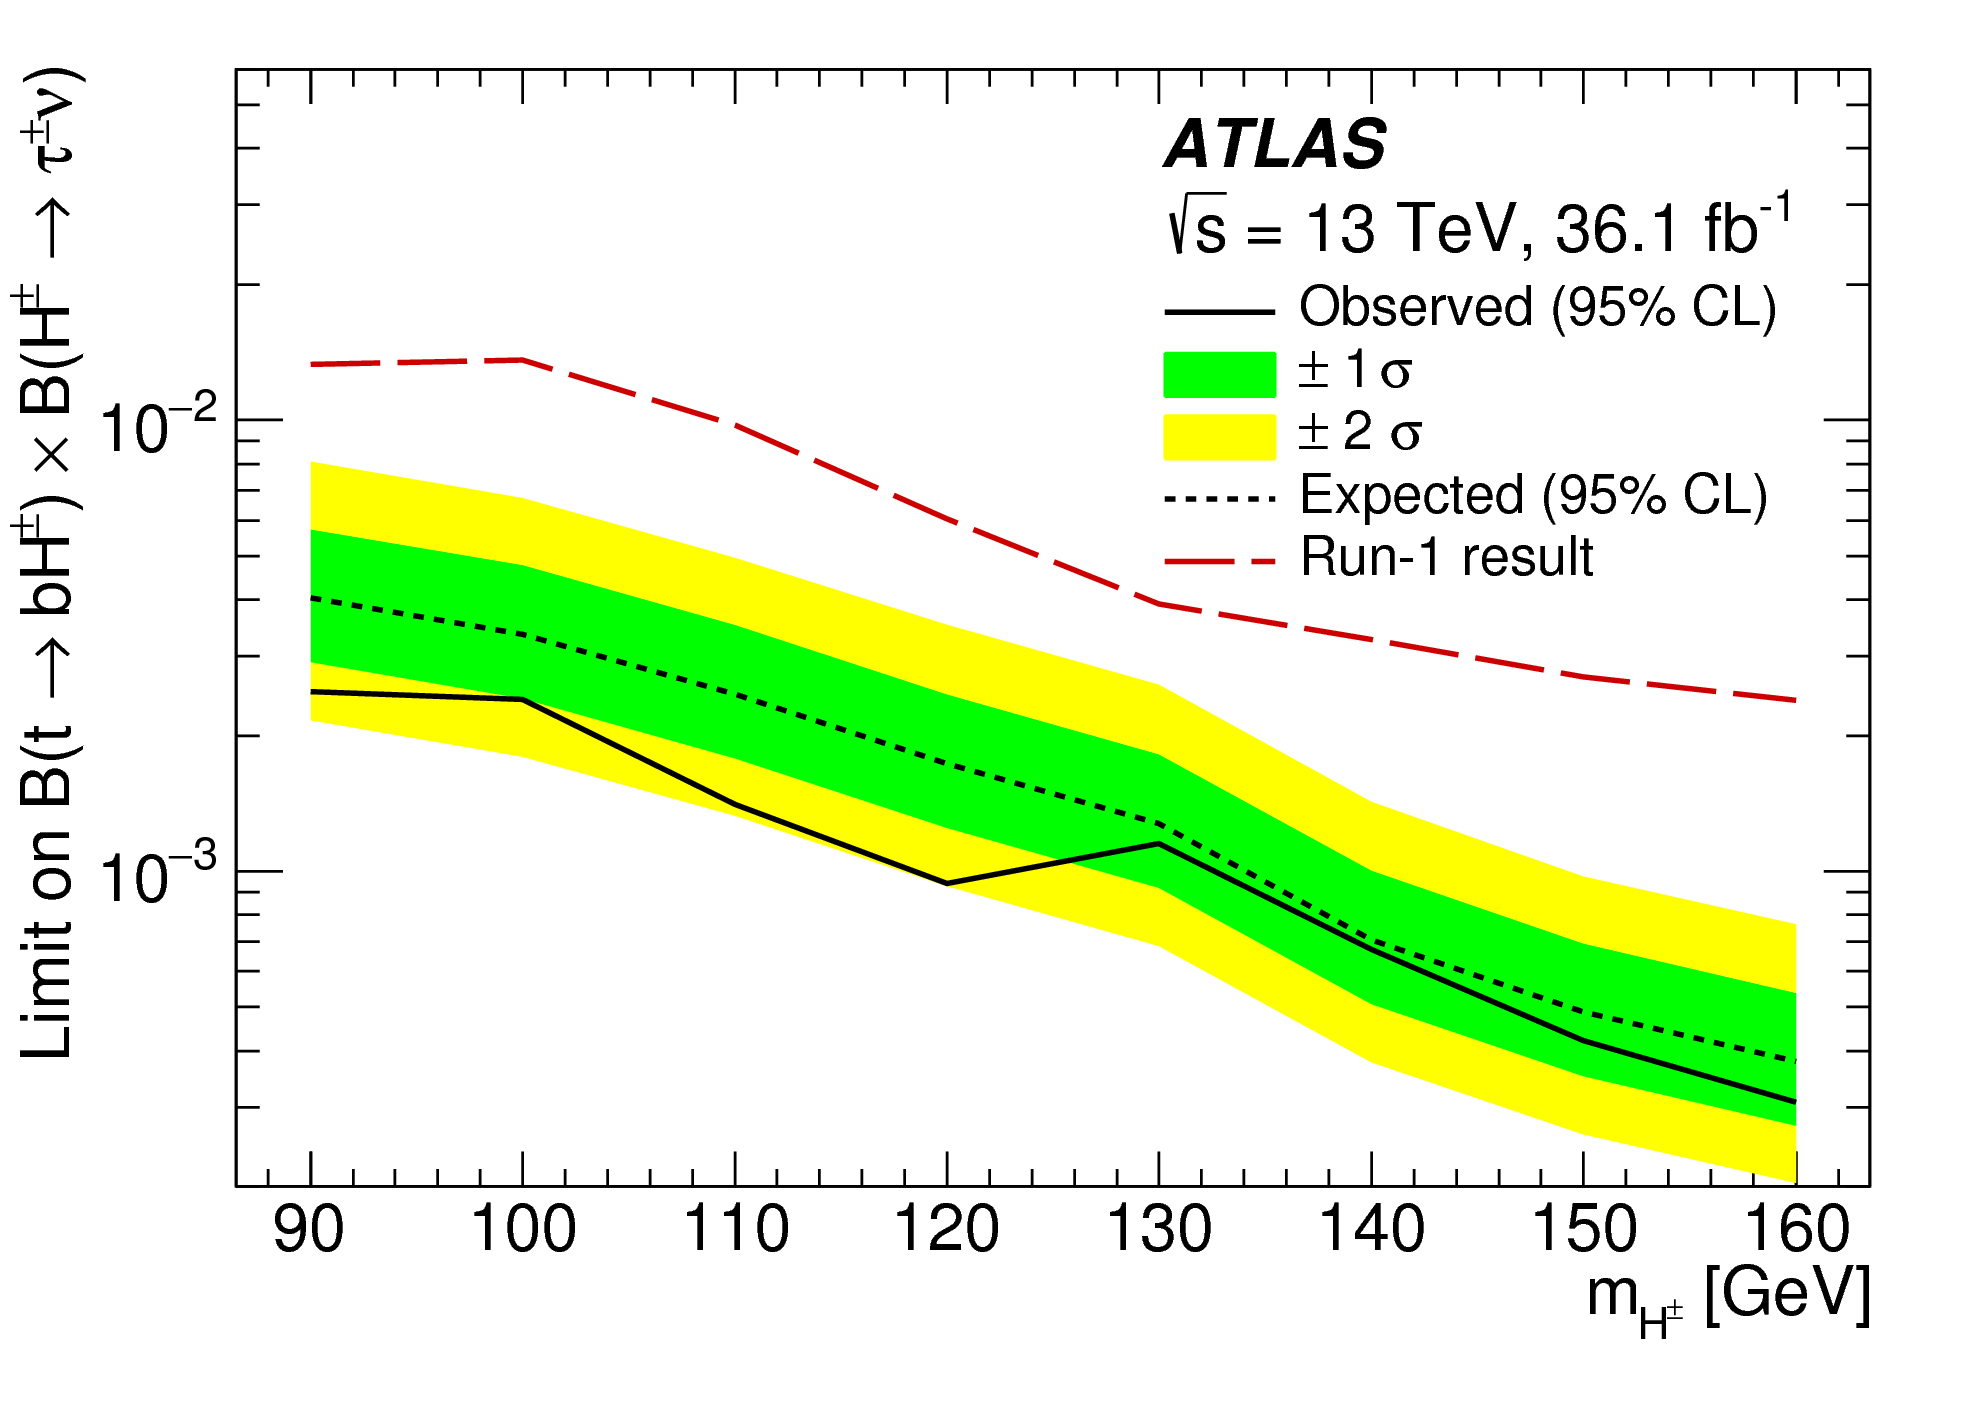
\includegraphics[width=.65\textwidth,keepaspectratio=true]{Limits/Combined_low_NoLabel_2018.png}
        % \column{.25\textwidth}
        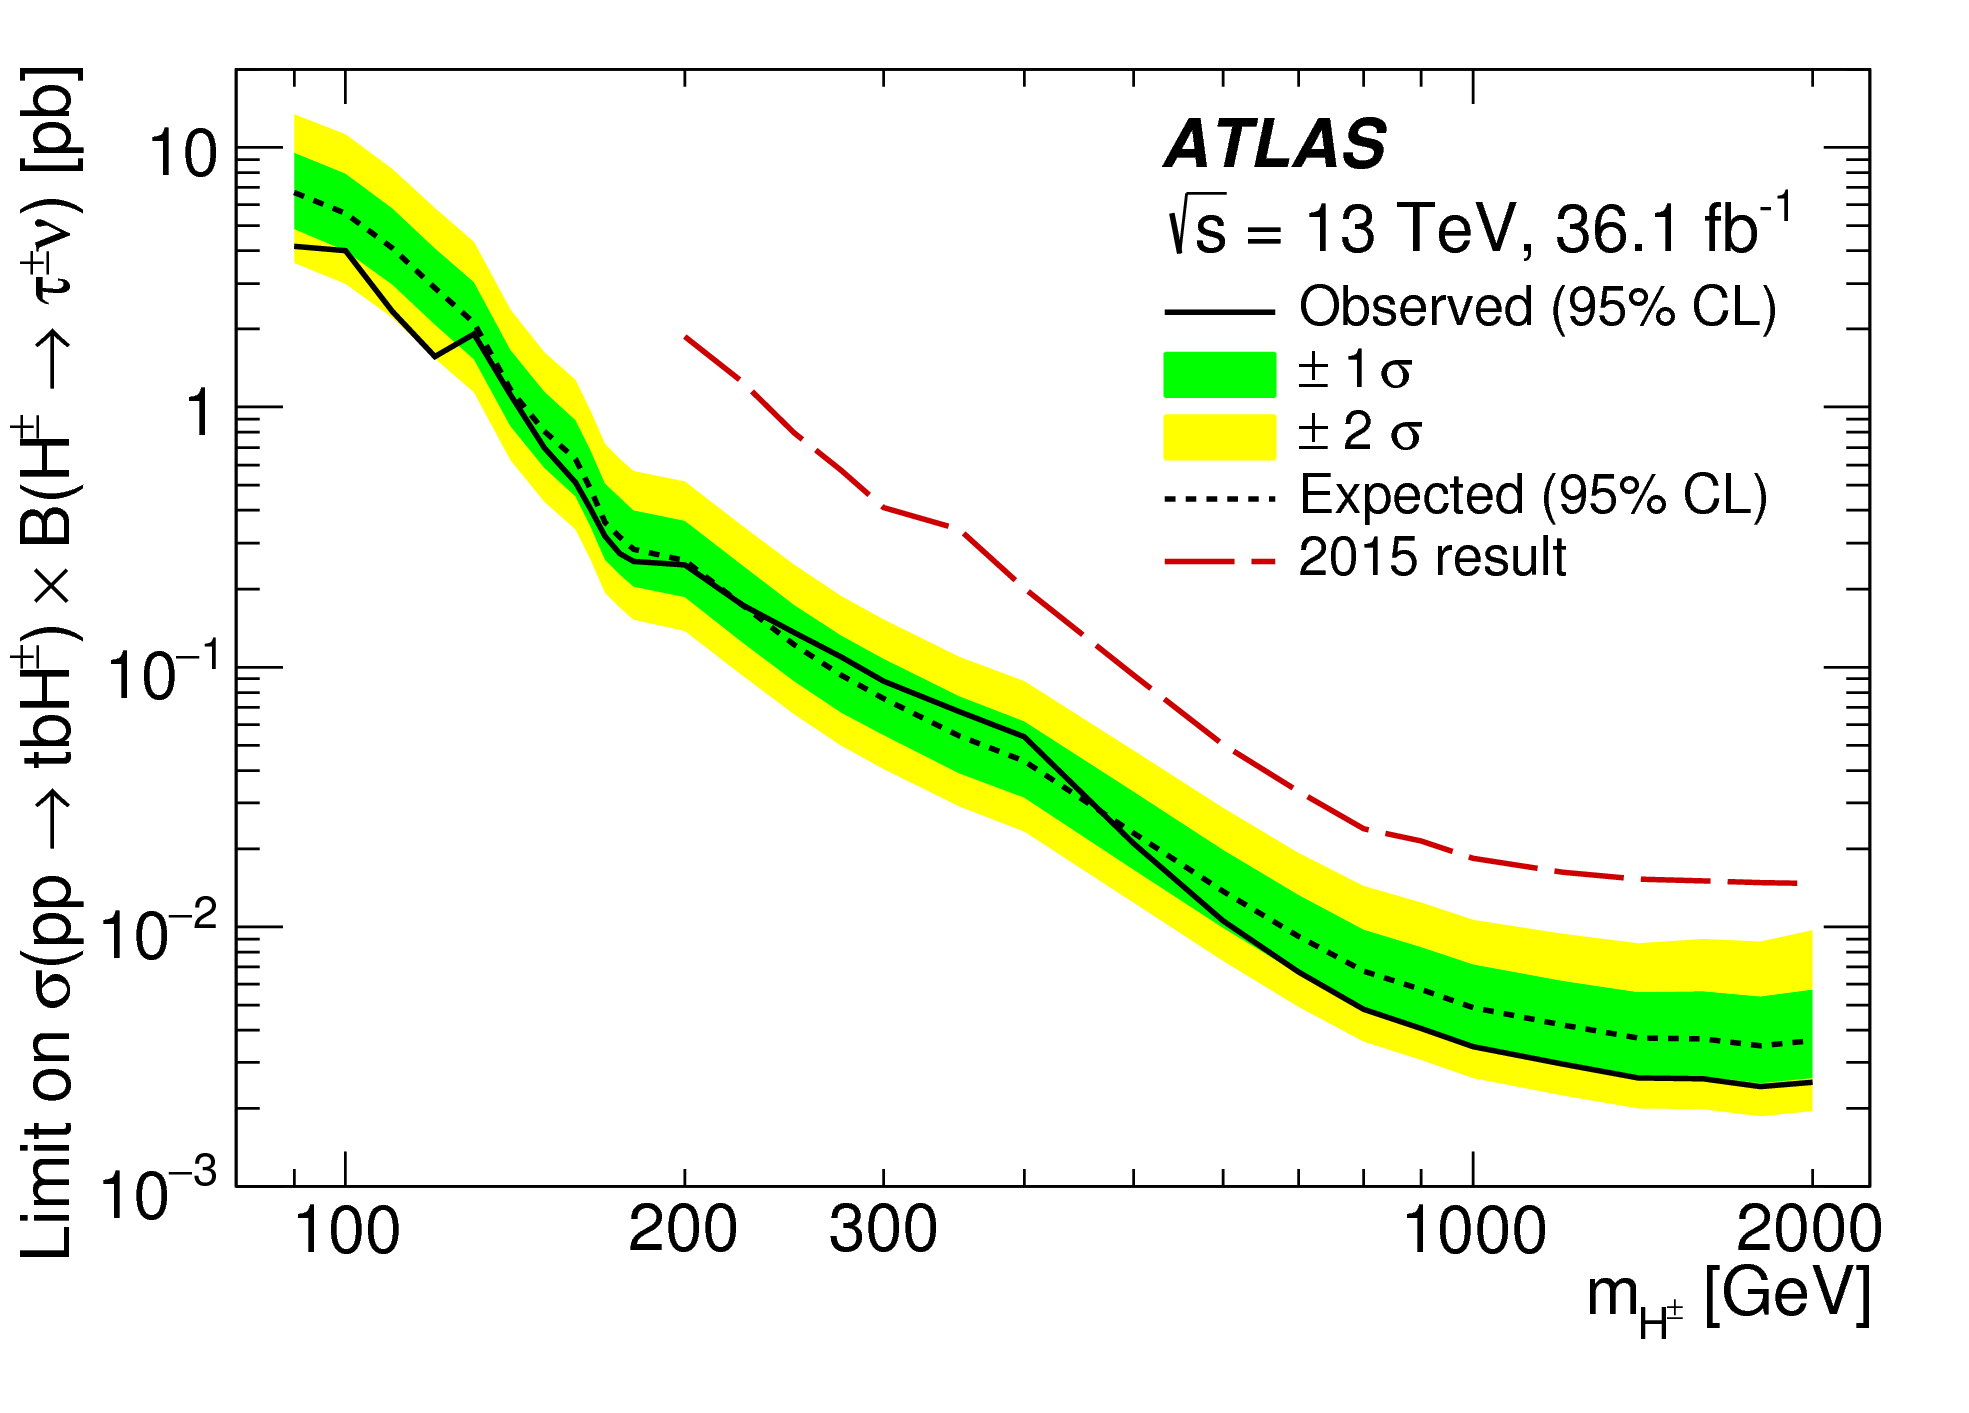
\includegraphics[width=.65\textwidth,keepaspectratio=true]{Limits/Combined_CrossSection_2018.png}
        \column{.5\textwidth}
        \centering
        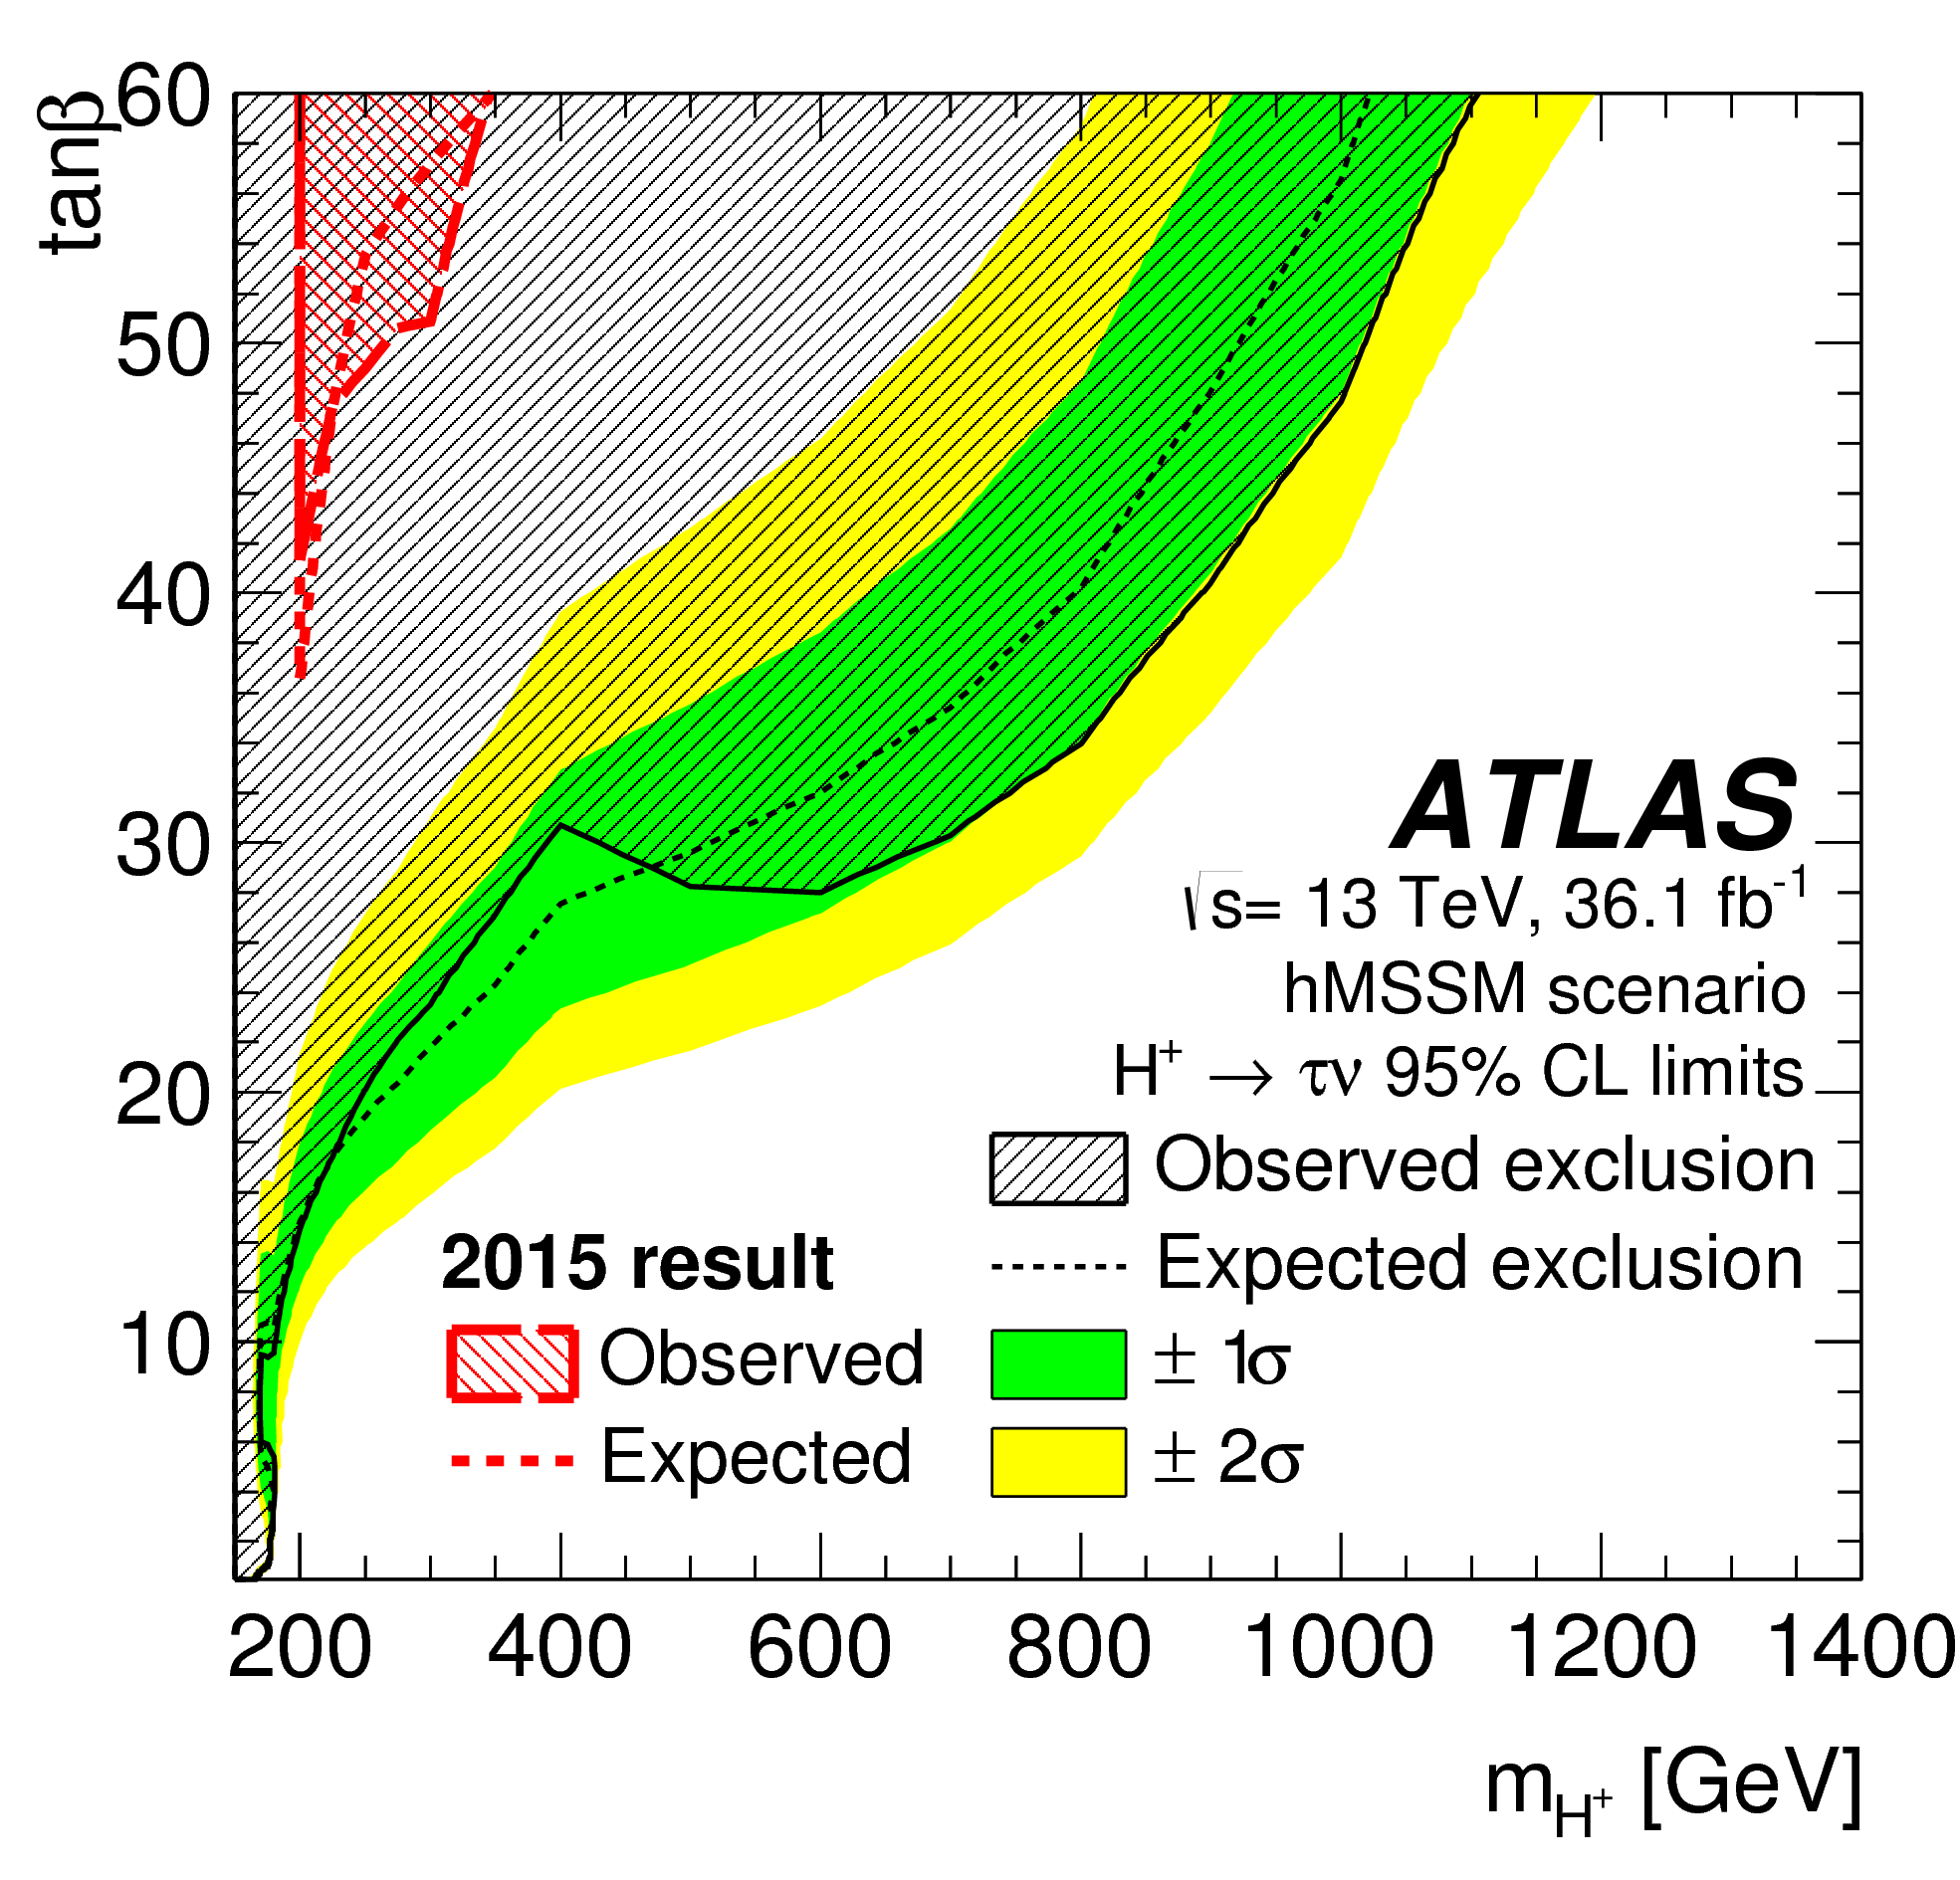
\includegraphics[width=\textwidth,keepaspectratio=true]{Limits/tanB_Limit_2018.png}
      \end{columns}
    \end{frame}

\section{Experimental Apparatus }

  \subsection{LHC }

    \begin{frame}[t]{Large Hadron Collider}

    \end{frame}

  \subsection{ATLAS }

    \begin{frame}[t]{The ATLAS Detector}

    \end{frame}

    \begin{frame}[t]{Inner Detector}

    \end{frame}

    \begin{frame}[t]{Calorimeters}

    \end{frame}

    \begin{frame}[t]{Tile Calorimeter}

    \end{frame}

    \begin{frame}[t]{Muon System}

    \end{frame}

    \begin{frame}[t]{Trigger System}

    \end{frame}

\section{Simulation }
  
  \begin{frame}[t]{Monte Carlo Simulation}

  \end{frame}

\section{Event Reconstruction }
  
  \begin{frame}[t]{Particle Identification}

  \end{frame}

\section{\HpmLong }
  
  \begin{frame}[t]{Analysis Overview}
      \begin{columns}[t]

        \column{.75\textwidth}
            \vspace{-20mm}
            \begin{itemize}
              \item Search for singly charged \Hpm decaying to \taunu over a wide mass range
                \begin{itemize}
                  \item Low mass $ (\mHpm < m_{t})$:
                  % \begin{itemize}
                  %   \item $90 \leq m_{H^{\pm}} \leq 130$ GeV
                  % \end{itemize}
                  \item Intermediate mass*  $(\mHpm \simeq m_{t})$
                  % \begin{itemize}
                  %   \item $140 \leq m_{H^{\pm}} \leq 190$ GeV
                  % \end{itemize}
                  \item High mass $(\mHpm > m_{t})$
                  % \begin{itemize}
                  %   \item $200 \leq m_{H^{\pm}} \leq 2000$ GeV
                  % \end{itemize}
                \end{itemize}
              % \item Associated $\tau$ is required to decay hadronically
              \item Dominant backgrounds
              \vspace{-3mm}
            \begin{table}
              \tiny
              \resizebox{\linewidth}{!}{
              \rowcolors{1}{}{NIUgray}
              \begin{tabular}{l | l}
              \textbf{Backgrounds w/ prompt hadronic $\tau$} & \textbf{Backgrounds w/ fake $\tau$} \\
              \hline \hline
              $t\bar{t}$ estimated with MC       & Fake $j \rightarrow \tau$ estimated with data driven fake factor method \\
              $V+jets$ estimated with MC         & Fake $\ell \rightarrow \tau$ estimated with MC, validated on $Z \rightarrow ee$\\
              VV estimated with MC & \\
              \end{tabular}}
            \end{table}
            \item MVA score is used as the final discriminant 
            % \item This talk will cover $36.1 \mathrm{fb}^{-1}$ and the current edition of this analysis
            \end{itemize}

            \vspace{-.45cm}
            \begin{table}
              \footnotesize
              \resizebox{\linewidth}{!}{
              \rowcolors{1}{}{NIUgray}
              \begin{tabular}{l | l | l | l | l | l | l | l | l | l | l | l} 
                \textbf{Sub-Channel} \\ \hline \hline
                \textbf{$\tau + jets$ SR } & $E^{miss}_{T}$ Trigger & \specialcell{1 hadronic $\tau$ \\ $p_{T}^{\tau} > 40$ GeV} & \specialcell{0 $\ell$ (e or $\mu$) \\ $p_{T}^{\ell} > 20$ GeV} & \specialcell{$\geq$ 3 jets \\ $p_{T}^{j} > 25$ GeV} & \specialcell{$\geq$ 1 b-jets \\ $p_{T}^{b-jet} > 25$ GeV}  & \Etm$ > 150$ GeV & $m_{T}(\tau,E^{miss}_{T}) > 50$ GeV \\ \hline
                \textbf{$\tau + \ell$ SR} & Single Lepton Trigger &   \specialcell{1 hadronic $\tau$ \\ $p_{T}^{\tau} > 30$ GeV} & \specialcell{1 $\ell$ (e or $\mu$) \\ $p_{T}^{\ell} > 30$ GeV} & \specialcell{$\geq$ 1 jet  \\ $p_{T}^{j} > 25$ GeV} & \specialcell{$\geq$ 1 b-jets \\  $p_{T}^{b-jet} > 25$ GeV} & \Etm$ > 50$ GeV & Opposite sign $\tau$ and $\ell$ \\ \hline
              \end{tabular}}
            \end{table}

            % \vspace{.3cm}
            \tiny *: First time probed experimentally \textcolor{blue}{\href{https://link.springer.com/article/10.1007/JHEP09(2018)139}{JHEP 09(2018)139}}

          \column{.25\textwidth}
          \centering
          \tiny
          \fcolorbox{black}{white}{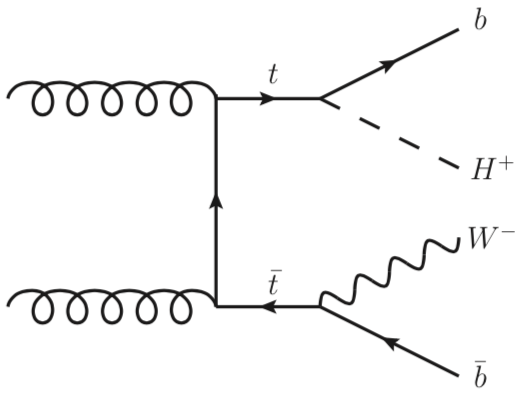
\includegraphics[width=.72\textwidth,keepaspectratio=true]{double_resonant_production_low_mass.png}}
          $m_{H^{\pm}} < m_{t}$
          \fcolorbox{black}{white}{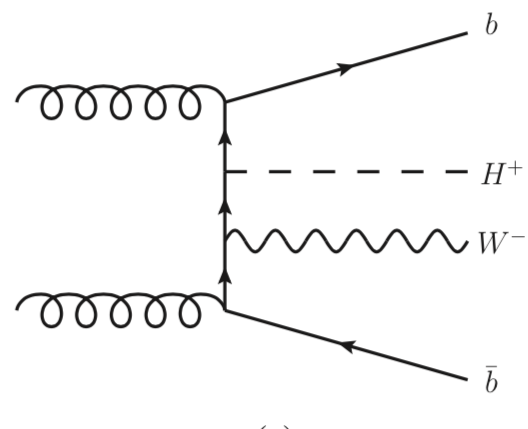
\includegraphics[width=.72\textwidth,keepaspectratio=true]{non_resonant_production_intermediate_mass.png}}
          $m_{H^{\pm}} \simeq m_{t}$
          \fcolorbox{black}{white}{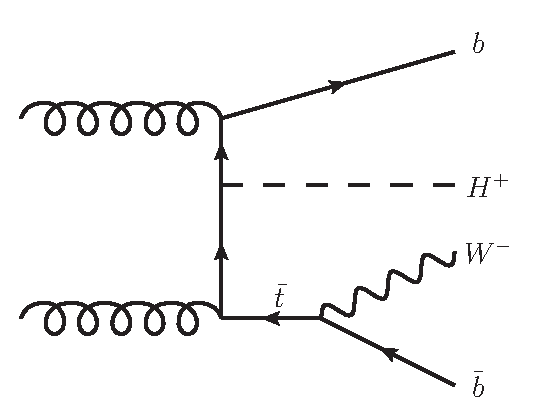
\includegraphics[width=.72\textwidth,keepaspectratio=true]{SingleResonant.pdf}}
          $m_{H^{\pm}} > m_{t}$
        \end{columns}
      \end{frame}

    \begin{frame}[t]{Updates to analysis since last publication}
      \begin{columns}
      \column{.6\linewidth}
        \begin{itemize}
          % \item Last publication using 2015+2016 data: \href{https://link.springer.com/article/10.1007/JHEP09(2018)139}{\textcolor{blue}{JHEP 09(2018)139}}
          % \item Using full Run-2 dataset
          \item Signal mass range extended 
          \begin{itemize}
            \item Previous: $90 \leq m_{H^{\pm}} \leq 2000$ GeV
            \item Current:  $80 \leq m_{H^{\pm}} \leq 3000$ GeV
          \end{itemize}
          \item Signal filtering applied in order to effectively increase the statistics in the signal regions
          \item New analysis framework centered around using modern Machine Learning tools
          \item Investigated new multivariate analysis techniques
          \item Updated derivations
          \vspace{-3.5mm}
          \begin{multicols}{2}
            \begin{itemize}
              \tiny
              \item RNN $\tau$ ID recommendations
              \item Updated b-tagging recommendations
              \item PFlow jets
              \item Latest Combined Performance recommendations
            \end{itemize}
          \end{multicols}
        \end{itemize}

      \column{.4\linewidth}
      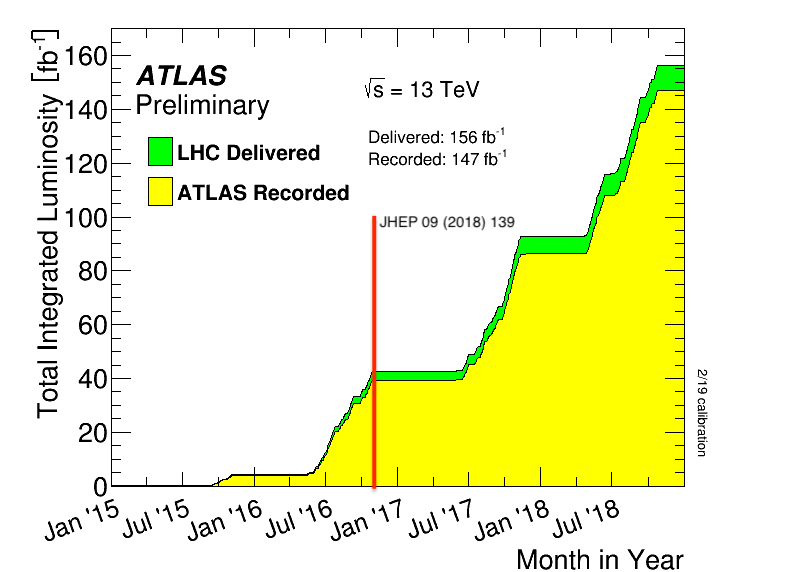
\includegraphics[width=1.1\textwidth,keepaspectratio=true]{intlumivstimeRun2.png}
      \end{columns}
    \end{frame}

    \begin{frame}[t]{Signal Acceptance}
      \begin{columns}
      \column{.5\textwidth}

      \column{.5\textwidth}
        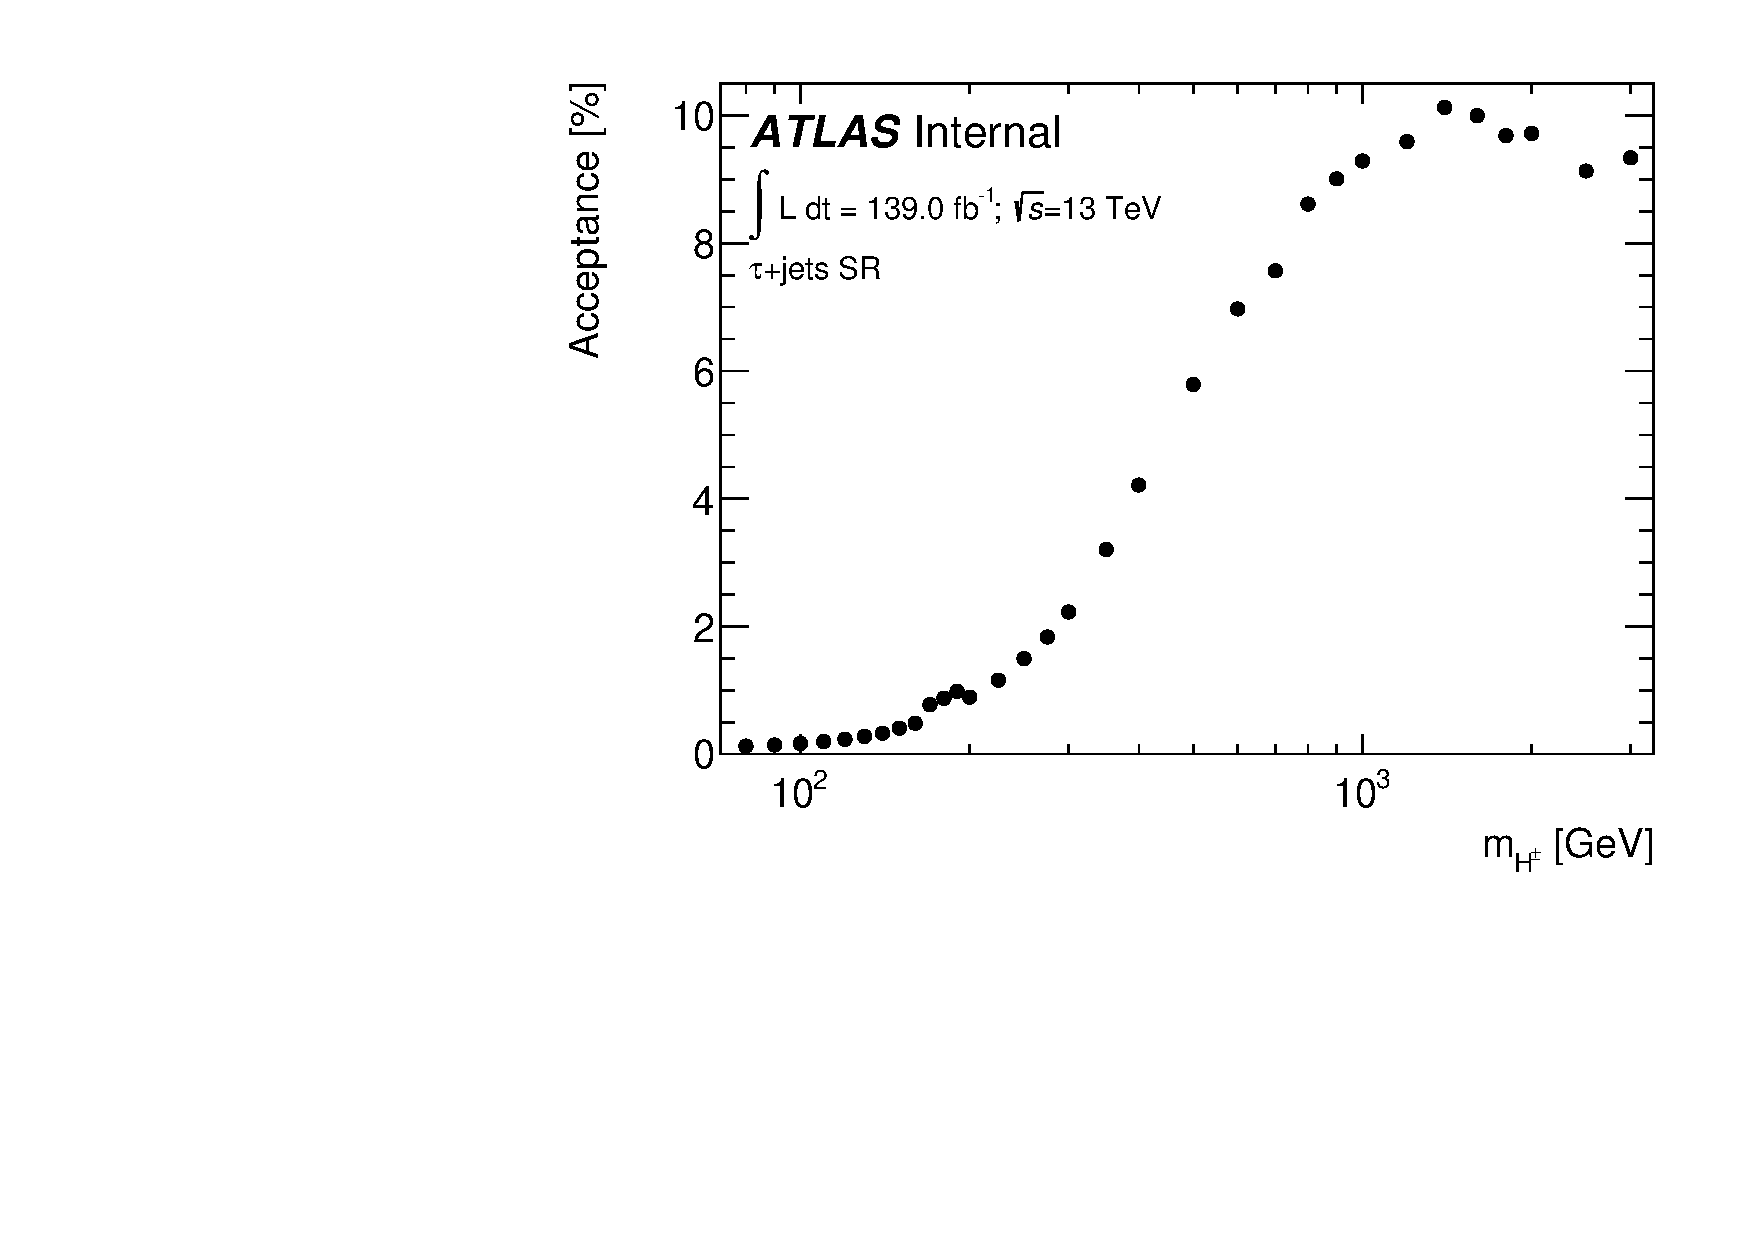
\includegraphics[height=.4\textheight,keepaspectratio=true]{/Users/eparrish/Work/thesis/chapters/chapter6_HPlus/images/Signal_Acceptance_Efficiency_SR_TAUJET.pdf}
        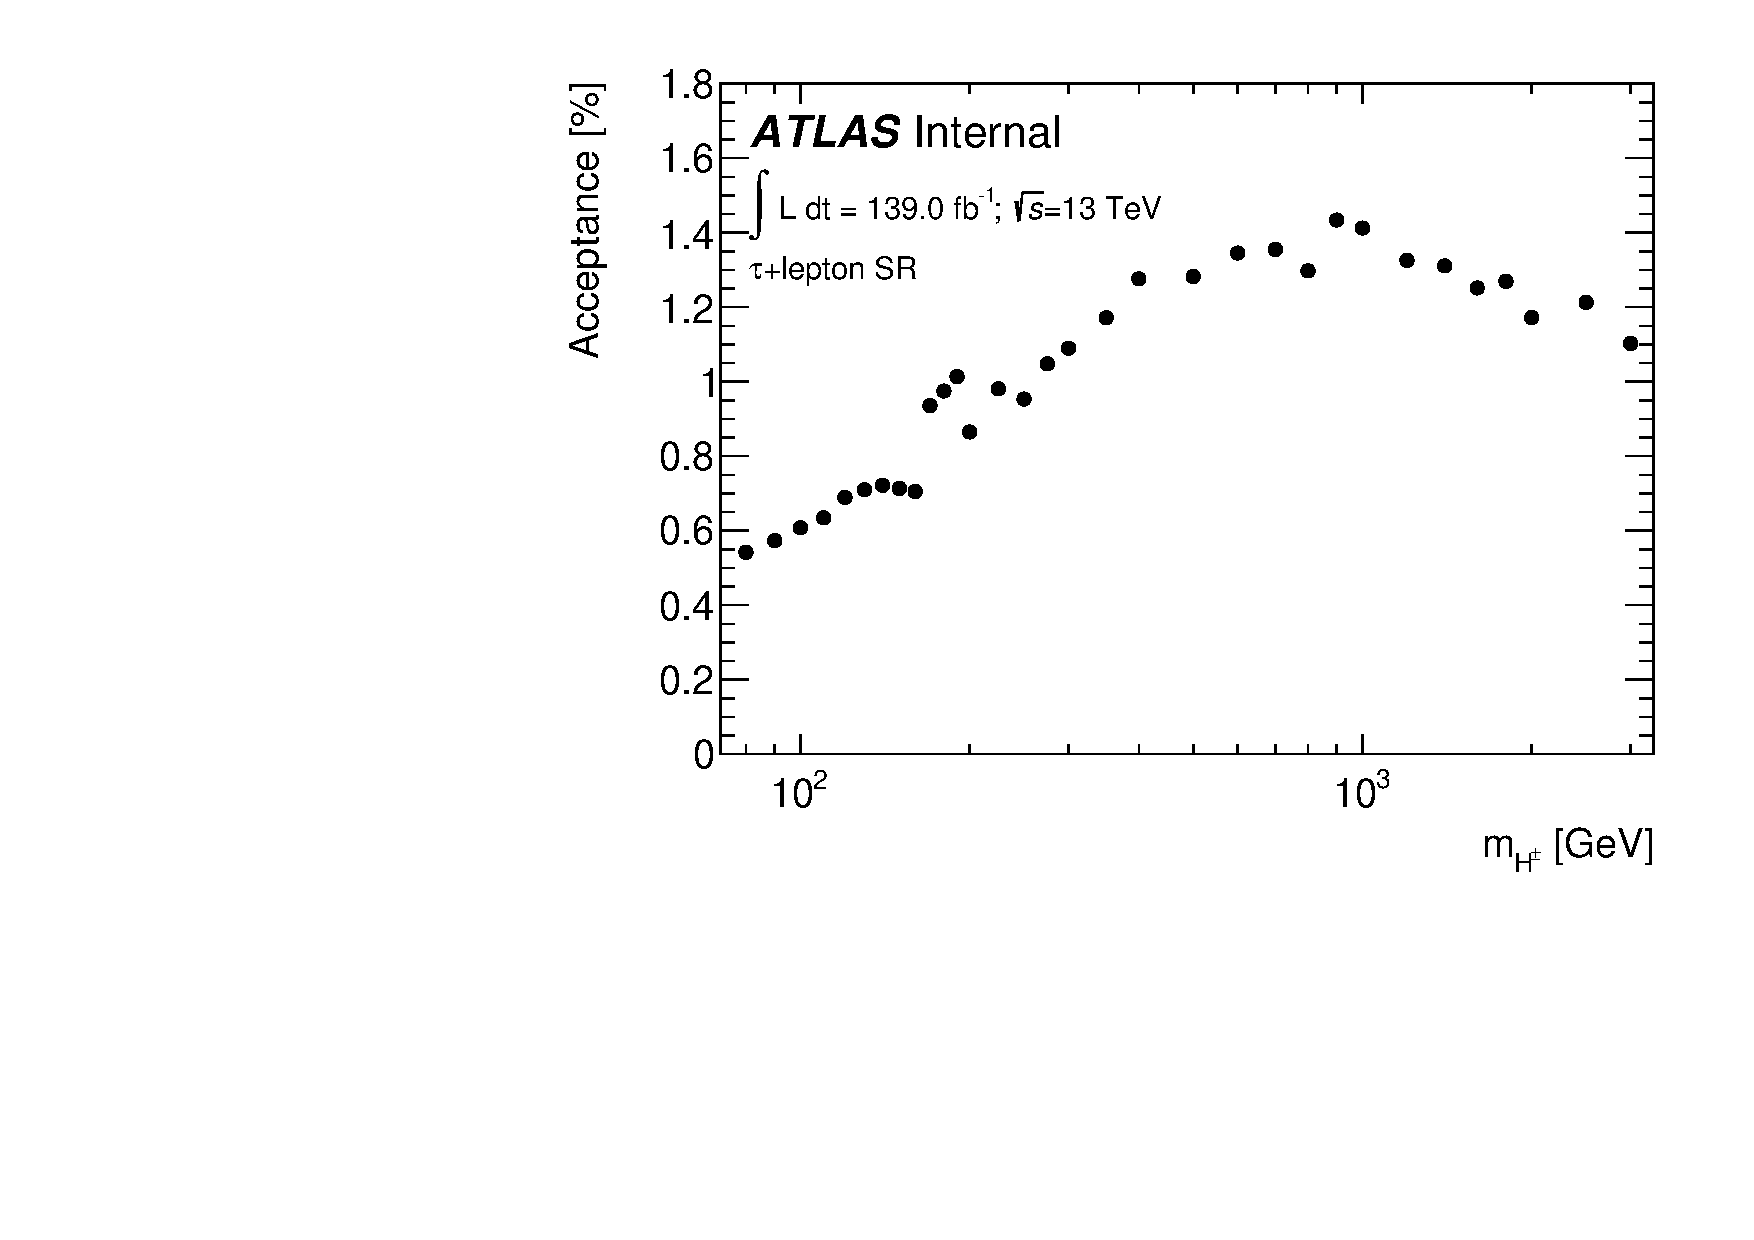
\includegraphics[height=.4\textheight,keepaspectratio=true]{/Users/eparrish/Work/thesis/chapters/chapter6_HPlus/images/Signal_Acceptance_Efficiency_SR_TAULEP.pdf}

      \end{columns}
    \end{frame}

  \subsection{$j \rightarrow \tau$ Fakes}

    \begin{frame}[t]{Background Estimation: $j \rightarrow \tau$ Fakes}
      \begin{columns}[t]
      \column[t]{.8\textwidth}
        \vspace{-3.5cm}
        \begin{itemize}
          \item Extract Fake-Factors $FF = \frac{N^{CR}_{\tau_{had-vis}}}{N^{CR}_{\bar{\tau}_{had-vis}}}$ from two orthogonal control regions:
            \begin{table}
              \tiny
              \resizebox{.42\linewidth}{!}{
              \rowcolors{1}{}{NIUgray}
              \begin{tabular}{l | l} 
              \textbf{Multi-Jet (gluon enriched)} & \textbf{W+Jets (quark enriched)} \\ 
              \hline \hline
              $E^{miss}_{T}$ or Multi-Jet trigger & Single lepton triggers \\
              $\geq 1 \tau_{had}, p_{T}^{\tau} > 30$ GeV & $\geq 1 \tau_{had}, p_{T}^{\tau} > 30$ GeV \\
              $\geq 3$  jets &  $\geq 1 $ jet\\
              0 b-jets & 0 b-jets \\
              % 0 $\ell$ & 1 $\ell$, $p^{\ell}_{T}>30$ GeV \\
              % $E^{miss}_{T} < 80$ GeV & 1 $\tau$ \\
              % $m_{T}(\tau,E^{miss}_{T}) > 50$ GeV &  $60 < m_{T}(\ell,E^{miss}_{T}) < 160$ GeV\\
              \end{tabular}}
            \end{table}
          \item Combine the two Fake-Factors via the template fit method:
          \begin{itemize}
            % \item $FF^{comb}_{i}=\alpha^{Multi-Jet}_{i} FF^{Multi-Jet}_{i} + [1-\alpha^{Multi-Jet}_{i}]FF^{W+jets}_{i}$
            \item Find two separate templates for anti-$\tau$ in each CR
            \item Fit both templates to the shape of the anti-$\tau$ in the SR
            \item Lowest $\chi^2$ of the fit defines $\alpha_{MJ}$ value and the corresponding error
          \end{itemize}
        \end{itemize}
            \centering
            \footnotesize
            $FF^{comb}_{i}=\alpha^{MJ}_{i} FF^{MJ}_{i} + [1-\alpha^{MJ}_{i}]FF^{W+jets}_{i}$
          \begin{itemize}
          \item Number of events with fake $\tau$ in the signal region is given by:
        \end{itemize}
          \centering
          \footnotesize
          $N^{\tau_{had-vis}}_{fakes} = \sum\limits_{i} N^{SR_{i}}_{\bar{\tau}_{had-vis}} FF_{i}$
      \column{.195\textwidth}
      \centering
      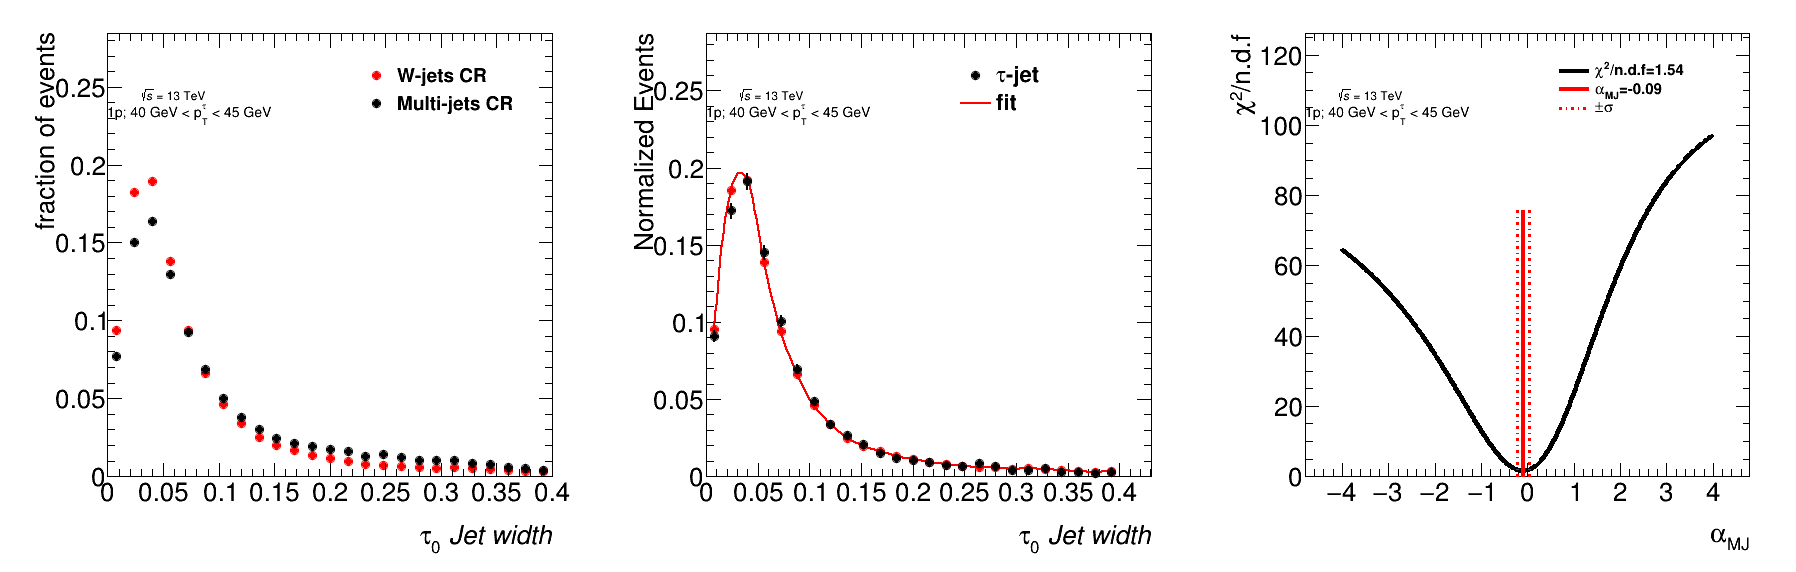
\includegraphics[trim={1.cm 0.cm 43.65cm 0.cm},clip,width=1.2\textwidth]{/Users/eparrish/Work/thesis/chapters/chapter6_HPlus/images/FFs/FFs_FIT_SR_TAUJET_1_40_45.png}
        \begin{itemize}
          \tiny
          \item $\bar{\tau_{0}}$ jet width used in $\alpha$ fitting of 1-prong and 3-prong $\bar{\tau}$
        \end{itemize}
         \begin{table}
          %   \tiny
            \resizebox{.65\textwidth}{!}{
            \rowcolors{1}{}{NIUgray}
            \begin{tabular}{l}
            \textbf{$\bar{\tau} \: ID$} \\
            \hline \hline
            $RNN \: Score > 0.01$ \\
            Not loose \\
            \end{tabular}}
          \end{table}
      \end{columns}
    \end{frame}

    % \begin{frame}[t]{Background Estimation: $j \rightarrow \tau$ Fakes}
    %   \begin{columns}
    %     \column[T]{.44\textwidth}
    %       \centering
    %       $\tau$+jets channel\\
    %       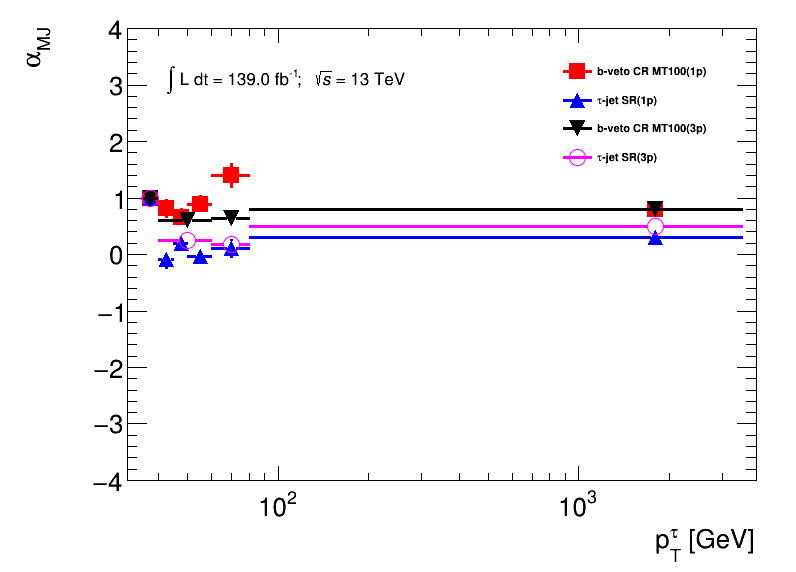
\includegraphics[width=.75\textwidth,keepaspectratio=true]{/Users/eparrish/Work/thesis/chapters/chapter6_HPlus/images/FFs/ALPHA_inclusive__taujet}\\
    %       \vspace{-0.1em}
    %       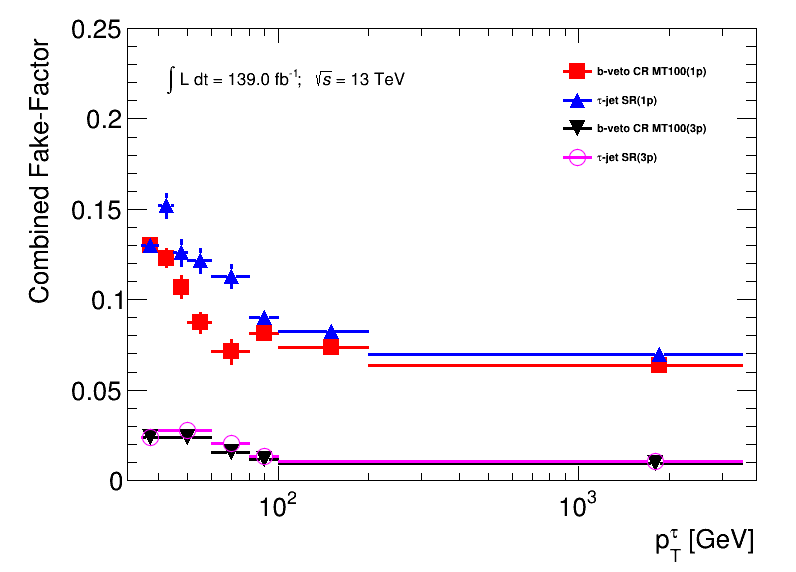
\includegraphics[width=.75\textwidth,keepaspectratio=true]{/Users/eparrish/Work/thesis/chapters/chapter6_HPlus/images/FFs/FFs_COM_inclusive__taujet}
    %     \column[T]{.44\textwidth}
    %       \centering
    %       $\tau$+lepton channel\\
    %       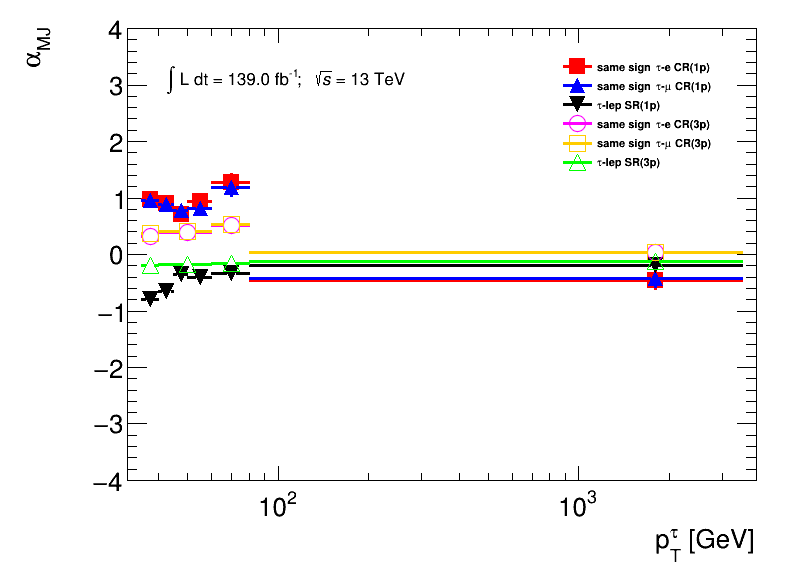
\includegraphics[width=.75\textwidth,keepaspectratio=true]{/Users/eparrish/Work/thesis/chapters/chapter6_HPlus/images/FFs/ALPHA_inclusive__taulep}\\
    %       \vspace{-0.1em}
    %       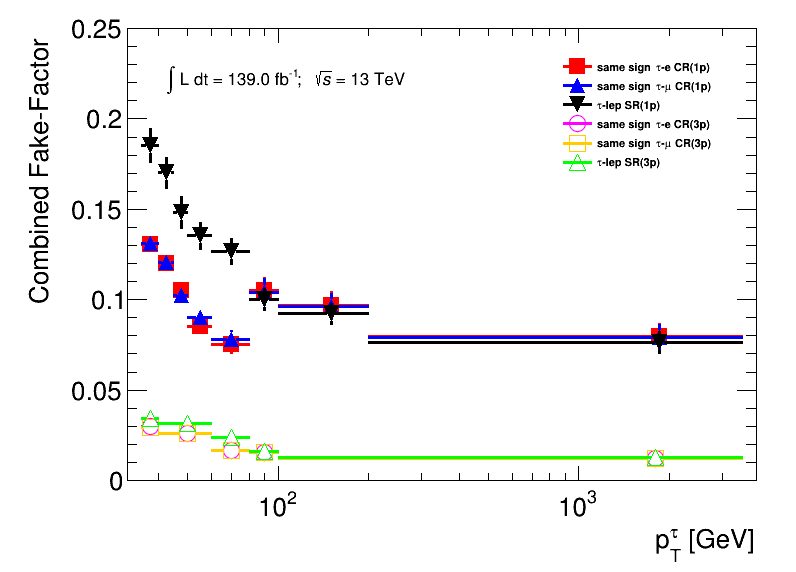
\includegraphics[width=.75\textwidth,keepaspectratio=true]{/Users/eparrish/Work/thesis/chapters/chapter6_HPlus/images/FFs/FFs_COM_inclusive__taulep}
    %   \end{columns}
    % \end{frame}

    % \begin{frame}[t]{Background Estimation: $j \rightarrow \tau$ Fakes}
    %     \begin{columns}
    %     \column{.11\textwidth}
    %     \begin{itemize}
    %       \tiny
    %       \item $\tau+jets$ w/ syst uncert.
    %       \vspace{2cm}
    %       \item $\tau+\ell$ w/ syst uncert.
    %     \end{itemize}
    %     \column{.25\textwidth}
    %     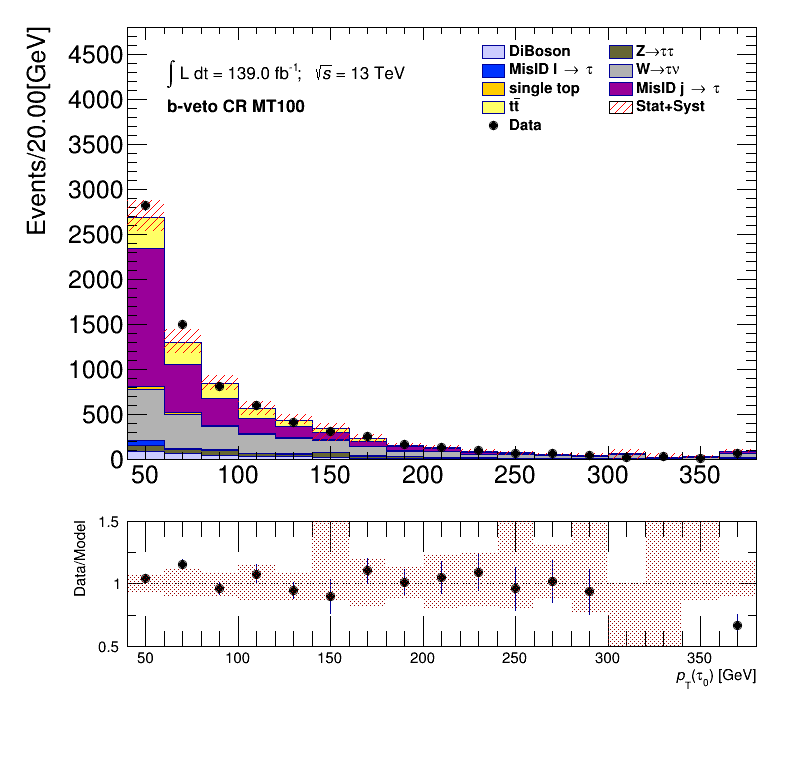
\includegraphics[height=.45\textheight,keepaspectratio=true]{/Users/eparrish/Work/thesis/chapters/chapter6_HPlus/images/taujets/tau_0_pt_BVETO_MT100.png}
    %     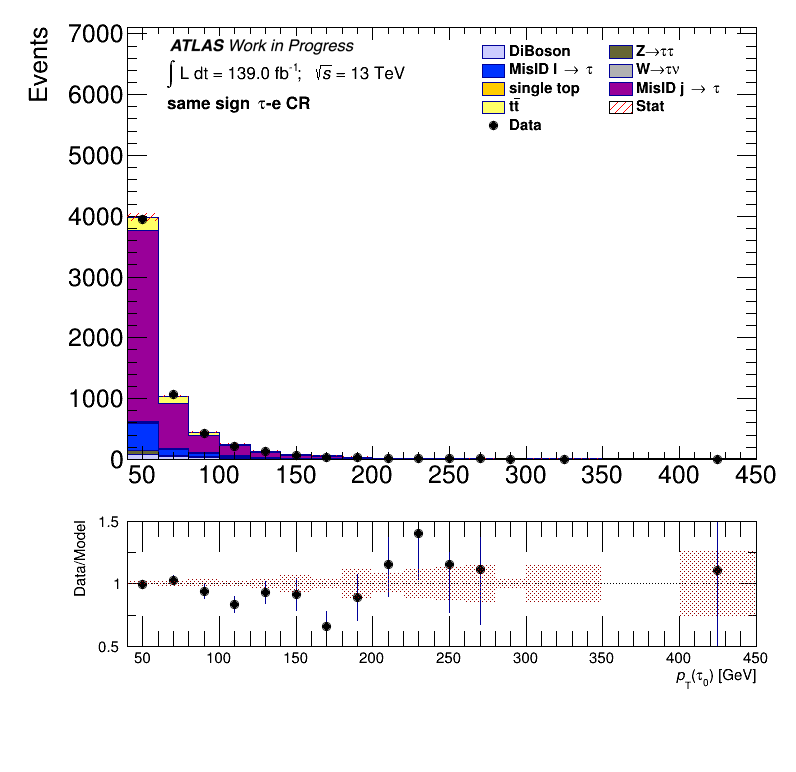
\includegraphics[height=.45\textheight,keepaspectratio=true]{/Users/eparrish/Work/thesis/chapters/chapter6_HPlus/images/taulep/tau_0_pt_SS_TAUEL.png}
    %     \column{.25\textwidth}
    %     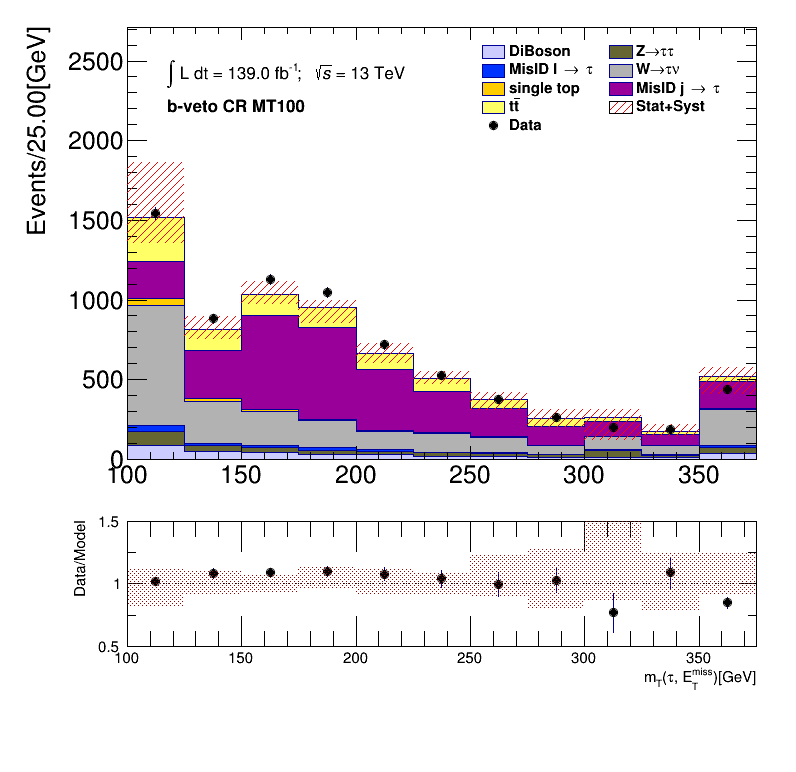
\includegraphics[height=.45\textheight,keepaspectratio=true]{/Users/eparrish/Work/thesis/chapters/chapter6_HPlus/images/taujets/tau_0_met_mt_BVETO_MT100.png}
    %     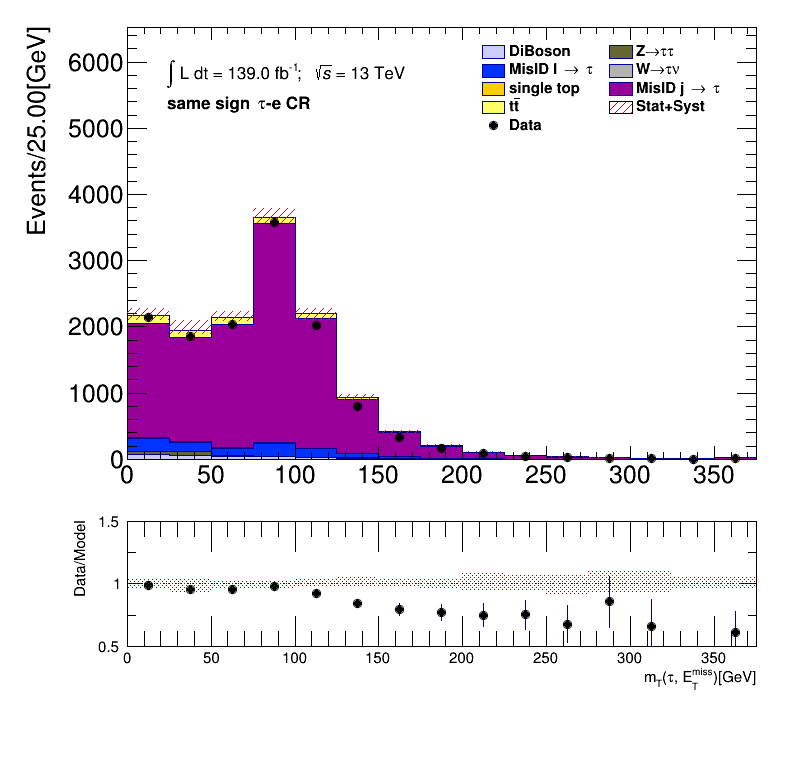
\includegraphics[height=.45\textheight,keepaspectratio=true]{/Users/eparrish/Work/thesis/chapters/chapter6_HPlus/images/taulep/tau_0_met_mt_SS_TAUEL.png}
    %     \column{.25\textwidth}
    %     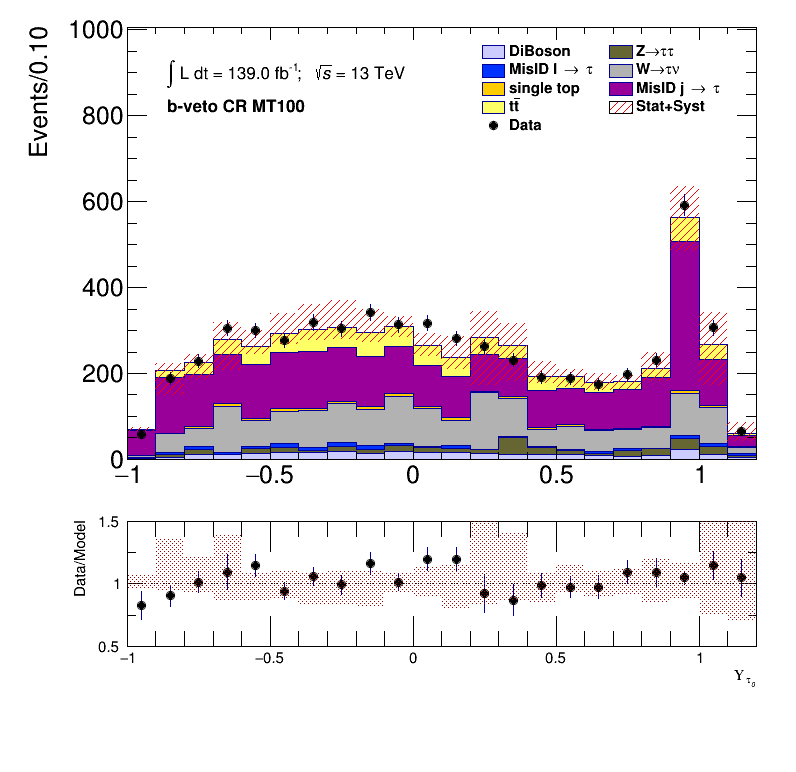
\includegraphics[height=.45\textheight,keepaspectratio=true]{/Users/eparrish/Work/thesis/chapters/chapter6_HPlus/images/taujets/tau_0_upsilon_BVETO_MT100.png}
    %     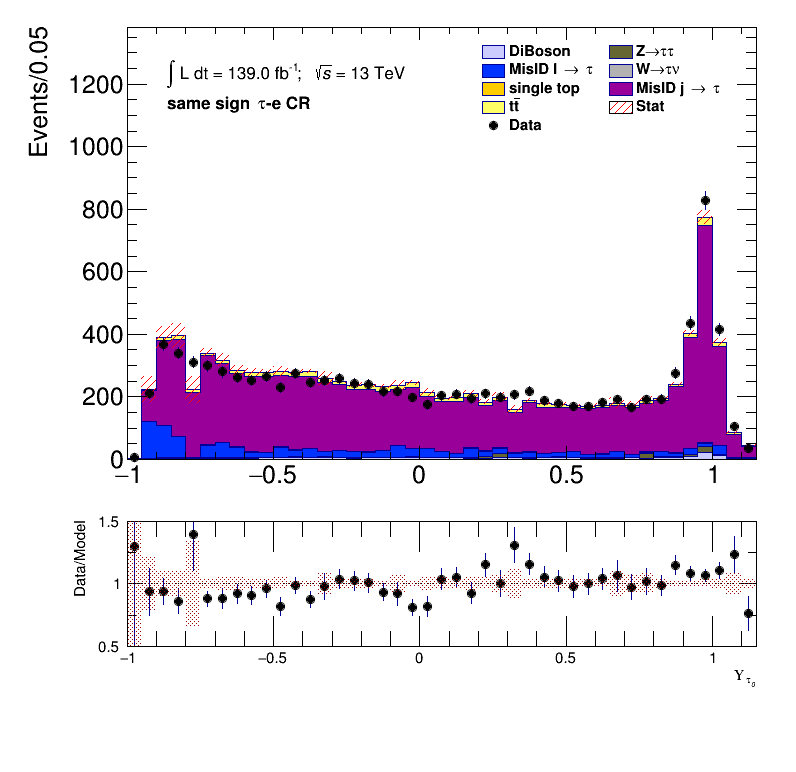
\includegraphics[height=.45\textheight,keepaspectratio=true]{/Users/eparrish/Work/thesis/chapters/chapter6_HPlus/images/taulep/tau_0_upsilon_SS_TAUEL.png}
    %   \end{columns}
    % \end{frame}

  \subsection{ Background Modeling }
    \begin{frame}[t]{$\tau+jets$ Background Modeling}
      % PLOTS FROM TAUJET
        \begin{columns}[t]

        \column{.25\textwidth}
        \includegraphics[height=.45\textheight,keepaspectratio=true]{/Users/eparrish/Work/thesis/chapters/chapter6_HPlus/images/taujets/tau_0_pt_TTBAR.png}
        \includegraphics[height=.45\textheight,keepaspectratio=true]{/Users/eparrish/Work/thesis/chapters/chapter6_HPlus/images/taujets/tau_0_pt_WJETS.png}

        \column{.25\textwidth}
        \includegraphics[height=.45\textheight,keepaspectratio=true]{/Users/eparrish/Work/thesis/chapters/chapter6_HPlus/images/taujets/met_et_TTBAR.png}
        \includegraphics[height=.45\textheight,keepaspectratio=true]{/Users/eparrish/Work/thesis/chapters/chapter6_HPlus/images/taujets/met_et_WJETS.png}

        \column{.25\textwidth}
        \includegraphics[height=.45\textheight,keepaspectratio=true]{/Users/eparrish/Work/thesis/chapters/chapter6_HPlus/images/taujets/tau_0_pt_BVETO.png}
        \includegraphics[height=.45\textheight,keepaspectratio=true]{/Users/eparrish/Work/thesis/chapters/chapter6_HPlus/images/taujets/tau_0_pt_BVETO_MT100.png}


        \column{.25\textwidth}
        \includegraphics[height=.45\textheight,keepaspectratio=true]{/Users/eparrish/Work/thesis/chapters/chapter6_HPlus/images/taujets/met_et_BVETO.png}
        \includegraphics[height=.45\textheight,keepaspectratio=true]{/Users/eparrish/Work/thesis/chapters/chapter6_HPlus/images/taujets/tau_0_met_mt_BVETO_MT100.png}
        % \includegraphics[height=.45\textheight,keepaspectratio=true]{/Users/eparrish/Work/thesis/chapters/chapter6_HPlus/images/taujets/met_et_bveto100.png}

      \end{columns}
    \end{frame}

    \begin{frame}[t]{$\tau+\ell$ Background Modeling}
      % PLOTS FROM TAULEP
      \begin{columns}[t]

        \column{.25\textwidth}
        \includegraphics[height=.45\textheight,keepaspectratio=true]{/Users/eparrish/Work/thesis/chapters/chapter6_HPlus/images/taulep/met_et_DILEP_BTAG.png}
        \includegraphics[height=.45\textheight,keepaspectratio=true]{/Users/eparrish/Work/thesis/chapters/chapter6_HPlus/images/taulep/tau_0_pt_TAUEL_BVETO.png}

        \column{.25\textwidth}
        \includegraphics[height=.45\textheight,keepaspectratio=true]{/Users/eparrish/Work/thesis/chapters/chapter6_HPlus/images/taulep/lep_0_pt_DILEP_BTAG.png}
        \includegraphics[height=.45\textheight,keepaspectratio=true]{/Users/eparrish/Work/thesis/chapters/chapter6_HPlus/images/taulep/lep_0_pt_TAUEL_BVETO.png}

        \column{.25\textwidth}
        \includegraphics[height=.45\textheight,keepaspectratio=true]{/Users/eparrish/Work/thesis/chapters/chapter6_HPlus/images/taulep/tau_0_pt_SS_TAUEL.png}
        \includegraphics[height=.45\textheight,keepaspectratio=true]{/Users/eparrish/Work/thesis/chapters/chapter6_HPlus/images/taulep/tau_0_pt_SS_TAUMU.png}


        \column{.25\textwidth}
        \includegraphics[height=.45\textheight,keepaspectratio=true]{/Users/eparrish/Work/thesis/chapters/chapter6_HPlus/images/taulep/lep_0_pt_SS_TAUEL.png}
        \includegraphics[height=.45\textheight,keepaspectratio=true]{/Users/eparrish/Work/thesis/chapters/chapter6_HPlus/images/taulep/lep_0_pt_SS_TAUMU.png}

      \end{columns}
    \end{frame}

  \subsection{ MVA }

    \begin{frame}[t]{Parameterized Neural Networks}
      \begin{columns}
      \column{.75\textwidth}
      \begin{itemize}
      \small
      \item Background modeling and classifier training kept statistically independent via the k-fold method
      \begin{itemize}
        \item For this analysis $k=5$
      \end{itemize}
      \item Trained using MC for backgrounds with true $\tau$
      \item Data-driven $j \rightarrow \tau$ fakes included for $\geq$ 500 GeV 
      \item Parameterized Neural Networks (PNNs) can be trained and evaluated on an entire mass range
      \begin{itemize}
        \item Detailed information here: \href{https://arxiv.org/abs/1601.07913}{\textcolor{blue}{arXiv:1601.07913}}
      \end{itemize}
      \item Trained using Tensorflow backend for Keras
      % \item \mHpm is used as an input feature of the model
      % \item Allows one model to be used across entire \mHpm mass range
      \item Separate models trained on 1 prong and 3 prong $\tau$
      \item \taulep channel is trained inclusive for \tauel and \taumu
      % \item Many ongoing studies
      %   \begin{itemize}
      %     \item High level vs low level input features
      %     \item Cartesian vs $(\eta,\phi)$ coordinates
      %     \item Hyperparameter optimization
      %   \end{itemize}
      \end{itemize}
      \column{.25\textwidth}
      % \small
      % \includegraphics[width=\textwidth,keepaspectratio=true]{taulep_fullmass.pdf}
      \footnotesize
      % NETWORK IMAGE
      \centering      
      \begin{figure}
        \centering
        \begin{columns}
        \column{.90\textwidth}
        \includegraphics[width=.9\textwidth,keepaspectratio=true]{/Users/eparrish/Work/thesis/chapters/chapter6_HPlus/images/PNN_Diagram.png}  
        \column{.10\textwidth}
        \caption{\tiny \cite{PNN}}
        \end{columns}
      \end{figure}
      \includegraphics[width=0.75\linewidth,keepaspectratio=true]{/Users/eparrish/Work/thesis/chapters/chapter6_HPlus/images/kFoldDiagram_noValid.pdf}
      \begin{table}
        \resizebox{.65\linewidth}{!}{
        \rowcolors{1}{}{NIUgray}
        \begin{tabular}{c | c | c |}
          \toprule
          \multicolumn{3}{c}{\textbf{$\tau+\ell$ Input Variables}} \\ \hline \hline
          $\pt^{\tau}$ & $\eta^{\tau}$ & $\phi^{\tau}$ \\ \hline
          $\pt^{\ell}$ & $\eta^{\ell}$ & $\phi^{\ell}$ \\ \hline
          % $\pt^{\bjet}$ & $\eta^{\bjet}$ & $\phi^{\bjet}$  \\ \hline
          $\pt^{j_{0}}$ & $\eta^{j_{0}}$ & $\phi^{j_{0}}$  \\ \hline
          \Etm & $\phi^{\Etm}$ & $\pt^{j_{1}}$  \\ \hline
          $m^{\Hpm}_{Truth}$ & $\Upsilon^{\tau}$ & \\ \hline 
          \bottomrule
          \end{tabular}}
        \end{table}

        % \column{.5\textwidth}
        \begin{table}
        \resizebox{.65\linewidth}{!}{
        \rowcolors{1}{}{NIUgray}
        \begin{tabular}{c | c | c |}
          \toprule
          \multicolumn{3}{c}{\textbf{$\tau+jets$ Input Variables}} \\ \hline \hline
          $\pt^{\tau}$ & $\eta^{\tau}$ & $\phi^{\tau}$\\ \hline
          % $\pt^{\ell}$ & $\eta^{\ell}$ & $\phi^{\ell}$ & $E^{\ell}$ \\ \hline
          % $\pt^{\bjet}$ & $\eta^{\bjet}$ & $\phi^{\bjet}$ \\ \hline
          $\pt^{j_{0}}$ & $\eta^{j_{0}}$ & $\phi^{j_{0}}$ \\ \hline
          $\pt^{j_{1}}$ & $\eta^{j_{1}}$ & $\phi^{j_{1}}$ \\ \hline
          $\pt^{j_{2}}$ & $\eta^{j_{2}}$ & $\phi^{j_{2}}$ \\ \hline
          \Etm & $\phi^{\Etm}$ & $m^{\Hpm}_{Truth}$  \\ \hline
          $\Upsilon^{\tau}$ &  & \\ \hline 
          \bottomrule
          \end{tabular}}
        \end{table}
      % Limits in $\tau+lep$ comparing BDT, NN, and PNN
      % PNN contains Upsilon variable
      % NNs in this plot are non parameterized, using 5 mass bins
      % \includegraphics[width=\textwidth,keepaspectratio=true]{PNN_Preliminary_Pawel_Feb_20_2020.png}
      \end{columns}
    \end{frame}

    \begin{frame}[t]{Parameterized Neural Network vs Boosted Decision Tree}
      \begin{itemize}
        \item One model for entire mass range makes analysis less computationally expensive
        \item PNN can be evaluated on mass points that are not simulated
        \item Limits are preliminary, many fixes and changes have been implemented since
      \end{itemize}
      \begin{columns}
      \column{.5\textwidth}
      \centering
      \includegraphics[width=\textwidth,keepaspectratio=true]{/Users/eparrish/Work/thesis/chapters/chapter6_HPlus/images/Limits/exp_limit_log_taujet.pdf}
      \column{.5\textwidth}
      \centering
      \includegraphics[width=\textwidth,keepaspectratio=true]{/Users/eparrish/Work/thesis/chapters/chapter6_HPlus/images/Limits/Exp_Limit_log_taulep.eps}
      \end{columns}
    \end{frame}

    \begin{frame}[t]{PNN Input Variable Selection}
      \begin{table}[!thp]
        \begin{subtable}[c]{0.15\textwidth}
          \centering
          % \begin{tabular}{| c | c | c | c |}
       %      \multicolumn{4}{c}{\textbf{Set A Input Variables}} \\ \hline \hline
       %      $\pt^{\tau}$ & $\eta^{\tau}$ & $\phi^{\tau}$ & $E^{\tau}$ \\ \hline
       %      $\pt^{\ell}$ & $\eta^{\ell}$ & $\phi^{\ell}$ & $E^{\ell}$ \\ \hline
       %      $\pt^{\bjet}$ & $\eta^{\bjet}$ & $\phi^{\bjet}$ & $E^{\bjet}$ \\ \hline
       %      $\pt^{jet}$ & $\eta^{jet}$ & $\phi^{jet}$ & $E^{jet}$ \\ \hline
       %      \Etm & $\phi^{\Etm}$ & $\pt^{j_{1}}$ & $\Upsilon$  \\ \hline
       %      $\mHpm^{Truth}$ & & & \\ \hline 
      %     \end{tabular}
          \begin{tabular}{| c | c | c |}
            \multicolumn{3}{c}{\textbf{Set A Input Variables}} \\ \hline \hline
            $\pt^{\tau}$ & $\eta^{\tau}$ & $\phi^{\tau}$  \\ \hline
            $\pt^{\ell}$ & $\eta^{\ell}$ & $\phi^{\ell}$  \\ \hline
            $\pt^{\bjet}$ & $\eta^{\bjet}$ & $\phi^{\bjet}$  \\ \hline
            $\pt^{jet}$ & $\eta^{jet}$ & $\phi^{jet}$  \\ \hline
            \Etm & $\phi^{\Etm}$ & $\pt^{j_{1}}$  \\ \hline
            $\Upsilon$ & $\mHpm^{Truth}$ &  \\ \hline 
          \end{tabular}
          \subcaption{Set A of input variables}
        \end{subtable}

        \begin{subtable}[c]{0.25\textwidth}
          \centering
          \begin{tabular}{| l |}
            \hline
            \textbf{Set B Input Variables} \\
            \hline \hline
            $\Etm$  \\
            $\pt^{\tau}$  \\
            $\pt^{\bjet}$  \\
            $\pt^{\ell}$  \\
            $\Delta \phi_{\tau,\,\text{miss}}$  \\
            $\Delta \phi_{\bjet,\,\text{miss}}$  \\
            $\Delta \phi_{\ell,\,\text{miss}}$  \\
            $\Delta R_{\tau,\,\ell}$ \\
            $\Delta R_{\bjet,\,\ell}$ \\
            $\Delta R_{\bjet,\,\tau}$ \\
            $\Delta \phi_{\tau, \text{miss}} / \Delta \phi_{\text{jet}, \text{miss}}$  \\
            $\Upsilon$ \\
            $\mHpm^{Truth}$ \\ \hline
          \end{tabular}
          \subcaption{Set B of input variables}
        \end{subtable}
        % \caption{Two sets of kinematic variables used as input to the \gls{PNN} in the \taulep subchannel. $\Delta \phi_{X,\,\text{miss}}$ denotes the difference in azimuthal angle between a reconstructed object $X$ ($X = \tau,\,\bjet,\,\ell$) and the direction of the missing transverse momentum.}
        % \label{tab:taulep-input-variables-high-v-low}
      \end{table}
    \end{frame}

  \subsection{ PNN HPO }

    \begin{frame}[t]{PNN Hyperparameter Optimization}
      \begin{itemize}
        \item Performed in the $\tau+\ell$ sub-channel
        \item Used area under curve (AUC) of scores as figure of merit
        \begin{itemize}
          \item Averaged over 5 kfolds, standard deviation is taken from kfolds
          % \item AUC from 80 GeV to 500 GeV to optimize for low mass
        \end{itemize}
          \item Used early stopping for training
          \begin{itemize}
            \item $\Delta_{min}=0.00001$ and a patience of 10
            \item Best weights were kept
          \end{itemize}
        \item To make hyperparameter optimization (HPO) go quicker, ran multiple small grids of hparams
        \begin{itemize}
          \item Scan over activation functions and loss functions
          % \begin{itemize}
          %   \item Binary crossentropy gave best result
          % \end{itemize}
          \item Scan over dropout value
          % \begin{itemize}
          %   \item 0.1 gave best result
          % \end{itemize}
          \item Scan over activation function
          % \begin{itemize}
          %   \item LeakyReLU was best
          % \end{itemize}
          \item Scan over LeakyReLU $\alpha$
          % \begin{itemize}
          %   \item $\alpha=0.05$ gave best results
          % \end{itemize}
          \item Fixed alpha over more widths and depths
          \begin{itemize}
            \item AUC from 80 GeV to 500 GeV to optimize for low mass
          \end{itemize}
        \end{itemize}
      \end{itemize}
    \end{frame}

    \begin{frame}[t]{PNN Hyperparameter Optimization Search}
      \begin{itemize}
        \item LeakyReLU activation function has an $\alpha$ parameter
        \item Slope of negative portion
        \begin{itemize}
          \item Prevents neurons from "dying" by allowing negative weight values
        \end{itemize}
        \item Standard relu is where $\alpha=0$
      \end{itemize}
      \centering
      \includegraphics[height=.4\textheight,keepaspectratio=true]{Activation_prelu.svg.png}
    \end{frame}

    \begin{frame}[t]{PNN Hyperparameter Optimization}
      \begin{columns}
        \column{.4\textwidth}

        \begin{table}
          \resizebox{\linewidth}{!}{
          \rowcolors{1}{}{NIUgray}
            \begin{tabular}{c | c | c | c}
            Parameter  \\
            \hline
            activation function & softsign & relu & LeakyReLU \\ \hline
            loss function & \fcolorbox{red}{white}{binary crossentropy} & mean squared error & mean absolute error \\ \hline
            width & 32 & & \\ \hline
            depth & 10 & & \\ \hline
            \end{tabular}}
        \end{table}


        \begin{table}
          \resizebox{.75\linewidth}{!}{
          \rowcolors{1}{}{NIUgray}
            \begin{tabular}{c | c | c | c}
            Parameter  \\
            \hline
            width & 8 & 16 & 32 \\ \hline
            depth & 3 & 5 & 10 \\ \hline
            dropout & \fcolorbox{red}{white}{0.1} & 0.3 & \\ \hline
            activation function & softsign & & \\ \hline
            loss function & binary crossentropy & & \\ \hline 
            \end{tabular}}
        \end{table}

        \begin{table}
          \resizebox{.75\linewidth}{!}{
          \rowcolors{1}{}{NIUgray}
            \begin{tabular}{c | c | c | c}
            Parameter  \\
            \hline
            width & 32 & 64 & 128 \\ \hline
            depth & 2 & 3 & 4 \\ \hline
            dropout & 0.1 & & \\ \hline
            activation function & softsign & relu & \fcolorbox{red}{white}{LeakyReLU} \\ \hline
            batch size & 1025 &  & \\ \hline
            loss function & binary crossentropy  & & \\
            \end{tabular}}
        \end{table}


        \column{.6\textwidth}

        \begin{table}
          \resizebox{.75\linewidth}{!}{
          \rowcolors{1}{}{NIUgray}
          \begin{tabular}{c | c | c | c | c}
          Parameter  \\ 
          \hline
          width & 32 & 64 & 128 & \\ \hline
          depth & 2 & 3 & 4 &  \\ \hline
          $\alpha$ & 0.01 & \fcolorbox{red}{white}{0.05} & 0.001 & 0.005 \\ \hline
          batch size & 1024 & & & \\ \hline
          dropout & 0.1 & & & \\ \hline
          activation function & LeakyReLU &  &  &  \\ \hline
          loss function & binary crossentropy & & &  \\ \hline
          \end{tabular}}
        \end{table}

        \begin{table}
          \resizebox{.75\linewidth}{!}{
          \rowcolors{1}{}{NIUgray}
          \begin{tabular}{c | c | c | c | c}
          Parameter  \\ 
          \hline
          width & 32 & 64 & \fcolorbox{red}{white}{128} & 256 \\
          depth & 2 & \fcolorbox{red}{white}{3} & 4 & 5 \\
          batch size & 1024 &  & & \\ \hline
          dropout & 0.1 &  &  &  \\ \hline
          activation function & LeakyReLU &  &  &  \\ \hline
          $\alpha$ & 0.05 &  &  &  \\ \hline
          loss function & binary crossentropy & & &  \\ \hline
          \end{tabular}}
        \end{table}
      \end{columns}
    \end{frame}

    \begin{frame}{PNN Hyperparameter Optimization Results}
      \begin{table}
        \begin{center}
        \small
        \resizebox{\textwidth}{!}{
        \begin{tabular}{llrrrrrrrrrrrr}
        \toprule
        width & depth &         80 &       150 &       250 &       500 &       Avg &   LowMassAvg \\
        \midrule
          128 & 3 & 0.6661  $\pm$ 0.0000  & 0.8145  $\pm$ 0.0000  & 0.9031  $\pm$ 0.0000  & 0.9633  $\pm$ 0.0000  & 0.8876  $\pm$ 0.0000  & 0.8261  $\pm$ 0.0968  \\
          128 & 5 & 0.6492  $\pm$ 0.0000  & 0.8043  $\pm$ 0.0000  & 0.9078  $\pm$ 0.0000  & 0.9628  $\pm$ 0.0000  & 0.8861  $\pm$ 0.0000  & 0.8235  $\pm$ 0.1000  \\
          128 & 4 & 0.6593  $\pm$ 0.0000  & 0.8117  $\pm$ 0.0000  & 0.9012  $\pm$ 0.0000  & 0.9638  $\pm$ 0.0000  & 0.8858  $\pm$ 0.0000  & 0.8232  $\pm$ 0.0994  \\
          128 & 2 & 0.6444  $\pm$ 0.0000  & 0.8070  $\pm$ 0.0000  & 0.9075  $\pm$ 0.0000  & 0.9631  $\pm$ 0.0000  & 0.8857  $\pm$ 0.0000  & 0.8231  $\pm$ 0.1006  \\
          64 &  4 & 0.6576  $\pm$ 0.0050  & 0.8080  $\pm$ 0.0013  & 0.9052  $\pm$ 0.0045  & 0.9656  $\pm$ 0.0016  & 0.8857  $\pm$ 0.0002  & 0.8230  $\pm$ 0.0994  \\
          64 &  2 & 0.6528  $\pm$ 0.0066  & 0.8052  $\pm$ 0.0023  & 0.9057  $\pm$ 0.0032  & 0.9651  $\pm$ 0.0007  & 0.8855  $\pm$ 0.0004  & 0.8228  $\pm$ 0.0996  \\
          64 &  5 & 0.6538  $\pm$ 0.0050  & 0.8044  $\pm$ 0.0019  & 0.9058  $\pm$ 0.0037  & 0.9653  $\pm$ 0.0014  & 0.8853  $\pm$ 0.0005  & 0.8224  $\pm$ 0.0997  \\
          64 &  3 & 0.6520  $\pm$ 0.0067  & 0.8051  $\pm$ 0.0018  & 0.9042  $\pm$ 0.0044  & 0.9649  $\pm$ 0.0019  & 0.8853  $\pm$ 0.0011  & 0.8223  $\pm$ 0.0994  \\
          256 & 5 & 0.6536  $\pm$ 0.0010  & 0.8044  $\pm$ 0.0033  & 0.9036  $\pm$ 0.0042  & 0.9644  $\pm$ 0.0022  & 0.8844  $\pm$ 0.0002  & 0.8213  $\pm$ 0.1003  \\
          256 & 4 & 0.6434  $\pm$ 0.0000  & 0.8018  $\pm$ 0.0000  & 0.9017  $\pm$ 0.0000  & 0.9619  $\pm$ 0.0000  & 0.8823  $\pm$ 0.0000  & 0.8181  $\pm$ 0.1013  \\
          32 &  3 & 0.6369  $\pm$ 0.0094  & 0.7950  $\pm$ 0.0041  & 0.8977  $\pm$ 0.0032  & 0.9635  $\pm$ 0.0022  & 0.8798  $\pm$ 0.0012  & 0.8139  $\pm$ 0.1031  \\
          32 &  4 & 0.6384  $\pm$ 0.0037  & 0.7935  $\pm$ 0.0033  & 0.8986  $\pm$ 0.0037  & 0.9636  $\pm$ 0.0016  & 0.8799  $\pm$ 0.0009  & 0.8139  $\pm$ 0.1031  \\
          32 &  2 & 0.6399  $\pm$ 0.0058  & 0.7924  $\pm$ 0.0024  & 0.8983  $\pm$ 0.0033  & 0.9629  $\pm$ 0.0023  & 0.8796  $\pm$ 0.0004  & 0.8135  $\pm$ 0.1023  \\
          32 &  5 & 0.6350  $\pm$ 0.0077  & 0.7931  $\pm$ 0.0056  & 0.8981  $\pm$ 0.0022  & 0.9625  $\pm$ 0.0005  & 0.8792  $\pm$ 0.0011  & 0.8128  $\pm$ 0.1035  \\
          256 & 2 & 0.6320  $\pm$ 0.0044  & 0.7971  $\pm$ 0.0000  & 0.8939  $\pm$ 0.0034  & 0.9587  $\pm$ 0.0018  & 0.8781  $\pm$ 0.0002  & 0.8120  $\pm$ 0.1023  \\
        \bottomrule
        \end{tabular}}
        % \caption{\label{tab:pnn_hpo_aucs}
        % \glspl{AUC} of final \gls{HPO} grid. An error of 0 corresponds to only one job k-fold finishing training due to computational limits. The LowMassAvg error takes into account difference
        %   }
          \end{center}
      \end{table}
    \end{frame}

    \begin{frame}[c]{Final PNN Model Performance}
      \begin{columns}
      \column{.5\textwidth}
      \begin{table}
        \begin{center}
        \small
        \resizebox{.75\textwidth}{!}{
        \begin{tabular}{llrrrrrrrrrrrr}
        \toprule
        width & depth &  Avg &   LowMassAvg \\
        \midrule
          128  &  3 & 0.8876  $\pm$ 0.0000  & 0.8261  $\pm$ 0.0968  \\
          128 & 5 & 0.8861  $\pm$ 0.0000  & 0.8235  $\pm$ 0.1000  \\
          128 & 4 & 0.8858  $\pm$ 0.0000  & 0.8232  $\pm$ 0.0994  \\
          128 & 2 & 0.8857  $\pm$ 0.0000  & 0.8231  $\pm$ 0.1006  \\
          64 &  4 & 0.8857  $\pm$ 0.0002  & 0.8230  $\pm$ 0.0994  \\
          64 &  2 & 0.8855  $\pm$ 0.0004  & 0.8228  $\pm$ 0.0996  \\
          64 &  5 & 0.8853  $\pm$ 0.0005  & 0.8224  $\pm$ 0.0997  \\
          64 &  3 & 0.8853  $\pm$ 0.0011  & 0.8223  $\pm$ 0.0994  \\
          256 & 5 & 0.8844  $\pm$ 0.0002  & 0.8213  $\pm$ 0.1003  \\
          256 & 4 & 0.8823  $\pm$ 0.0000  & 0.8181  $\pm$ 0.1013  \\
          32 &  3 & 0.8798  $\pm$ 0.0012  & 0.8139  $\pm$ 0.1031  \\
          32 &  4 & 0.8799  $\pm$ 0.0009  & 0.8139  $\pm$ 0.1031  \\
          32 &  2 & 0.8796  $\pm$ 0.0004  & 0.8135  $\pm$ 0.1023  \\
          32 &  5 & 0.8792  $\pm$ 0.0011  & 0.8128  $\pm$ 0.1035  \\
          256 & 2 & 0.8781  $\pm$ 0.0002  & 0.8120  $\pm$ 0.1023  \\
        \bottomrule
        \end{tabular}}
        % \caption{\label{tab:pnn_hpo_aucs_short}
        % Average \glspl{AUC} of final \gls{HPO} grid. An error of 0 corresponds to only one job k-fold finishing training due to computational limits.
          % }
        \end{center}
      \end{table}
      \column{.5\textwidth}
      \includegraphics[height=.5\textheight,keepaspectratio=true]{/Users/eparrish/Work/thesis/chapters/chapter6_Hplus/images/AUC_Plots/model_GB_1024_channel_taulep_mass_80to3000_ntracks_1_nfolds_5_fold_4_nvars_19_batch_size_1024_epochs_1000_dense_layer_size_128_activation_function_LeakyRelu_depth_3_loss_binary_crossentropy_dropout_0.1_alpha_0.05.eps}
      \end{columns}
    \end{frame}

    

  \subsection{Systematic Uncertainties }

   \begin{frame}{Fake-factor method uncertainties}

      \begin{flushleft}
      Sources of systematic uncertainties associated with the FF method:
      \end{flushleft}

      \begin{itemize}
        \begin{multicols}{2}
        \item Statistical uncertainties
        \item True $\mathrm{\tau}$ contamination in the anti-$\mathrm{\tau}$ CR
        \item $\mathrm{\alpha_{MJ}}$ fitting procedure uncertainty
        \item Smirnov transformation
        \item Tau RNN Identification SF variation
        \item Heavy flavour jet fraction
        \end{multicols}
      \end{itemize}

      \begin{table}[!htb]
        \begin{center}
          \resizebox{.75\textwidth}{!}{
          \begin{tabular}{l|c|c||c|c||}
            &  \multicolumn{2}{c||}{\taujets}  & \multicolumn{2}{c||}{\taulep} \\
            \hline
            Source of uncertainty & Effect on yield & Shape & Effect on yield & Shape \\
            \hline\hline
            Fake factors: statistical uncertainties & 3.9$\%$ & \textcolor{red}{\ding{55}} & 3.2$\%$ & \textcolor{red}{\ding{55}}\\\hline
            Fake factors: True \tauhad in the anti-\tauhad CR & \begin{tabular}{c}+3.4\% \\-3.2\%\end{tabular} & \textcolor{red}{\ding{55}} & \begin{tabular}{c}+4\% \\-4.3\%\end{tabular} & \textcolor{red}{\ding{55}}\\\hline
            Fake factors: tau RNN Identification SF & 2.7$\%$ & \textcolor{red}{\ding{51}} & 2.7$\%$ & \textcolor{red}{\ding{51}}\\\hline
            Fake factors: $\alpha_\text{MJ}$ uncertainty & 3.6\% & \textcolor{red}{\ding{55}} & 1.9\% & \textcolor{red}{\ding{55}}\\\hline
            Fake factors: Smirnov transform & 0$\%$ & \textcolor{red}{\ding{51}} & 0$\%$ & \textcolor{red}{\ding{51}}\\\hline          
            Fake factors: heavy flavor jet fraction & 6$\%$ & \textcolor{red}{\ding{51}} & 5.53$\%$ & \textcolor{red}{\ding{51}}\\
          \end{tabular}}
        \end{center}
        % \caption{\label{tab:FF-syst-uncert}
          % Effect on the shape variation and the yields of systematic uncertainties associated with the data-driven fake
          % factor method, used to estimate the $j \to \tau$ background in the
         % \taujets and \taulep channel.
          % }
      \end{table}

      % \begin{flushleft}
      % % Evaluation of actual effect on the new PNN discriminant shape variation and the yields for uncertainty from heavy flavor jet fraction is work in progress.
      % \end{flushleft}
    \end{frame}

    \begin{frame}[t]{Sources of Systematic Uncertainty}
      \textcolor{red}{Table with systs}
    \end{frame}

  \subsection{Results }

    \begin{frame}{$H^{\pm} \rightarrow \tau\nu$ Expected Limits}
      \centering
      % \includegraphics[height=.9\textheight,keepaspectratio=true]{taulep_fullmass.pdf}
      \small
      % \begin{itemize}
      %   \item Limits with previous ntuples shown
      % \end{itemize}
      \begin{columns}
        \column{.5\textwidth}
        \centering
        \includegraphics[width=\textwidth,keepaspectratio=true]{/Users/eparrish/Work/thesis/chapters/chapter6_HPlus/images/Limits/139_vs_36_analysis_limits_PNN_vs_BDT_TauEl_logx.png} \\
        \centering
        $\tau+e$
        \column{.5\textwidth}
        \includegraphics[width=\textwidth,keepaspectratio=true]{/Users/eparrish/Work/thesis/chapters/chapter6_HPlus/images/Limits/139_vs_36_analysis_limits_PNN_vs_BDT_TauMu_logx.png}\\
        \centering
        $\tau+\mu$
      \end{columns}
    \end{frame}

    \begin{frame}{$H^{\pm} \rightarrow \tau\nu$ Expected Limits}
      \centering
      % \includegraphics[height=.9\textheight,keepaspectratio=true]{taulep_fullmass.pdf}
      \small
      \begin{columns}
        \column{.5\textwidth}
        \includegraphics[width=\textwidth,keepaspectratio=true]{/Users/eparrish/Work/thesis/chapters/chapter6_HPlus/images/Limits/139_vs_36_analysis_limits_PNN_vs_BDT_TauJets_logx.png} \\
        \centering
        $\tau+jets$
        \column{.5\textwidth}
        \includegraphics[width=\textwidth,keepaspectratio=true]{/Users/eparrish/Work/thesis/chapters/chapter6_HPlus/images/Limits/139_vs_36_analysis_limits_PNN_vs_BDT_TauLep_logx.png} \\
        \centering
        $\tau+\ell$
      \end{columns}
      \end{frame}

      \begin{frame}{$H^{\pm} \rightarrow \tau\nu$ Expected Limits}
      \centering
      \includegraphics[height=.75\textheight,keepaspectratio=true]{/Users/eparrish/Work/thesis/chapters/chapter6_HPlus/images/Limits/139_vs_36_analysis_limits_PNN_vs_BDT_Combined_logx.png} \\
      \centering
      Combined
    \end{frame}


\section{Conclusion }

  \begin{frame}[t]{Conclusions}
    \begin{itemize}
      \item New analysis strategy outperforms previous analysis by a factor of \textcolor{red}{XX}
      \item Analysis is still blinded
      \item Paper will be published soon
    \end{itemize}
  \end{frame}

  \begin{frame}{Thank You}
    \centering
    \includegraphics[height=7.4cm, keepaspectratio=true]{CERN_globe.jpeg}
  \end{frame}


%%%%%%%%%%%%%%%%%%%%%%%%%%%%%%%%%%%%%%%%%%%%%%%%%%%%%%%%%%%%%%%%%%%%%%%%%%%%%%%%%
%%%%%%%%%%%%%%%%%%%%%%%%%%%%%%%%%%%%%%%%%%%%%%%%%%%%%%%%%%%%%%%%%%%%%%%%%%%%%%%%%
%%%%%%%%%%%%%%%%%%%%%%%%%%%%%%%%%%%%%%%%%%%%%%%%%%%%%%%%%%%%%%%%%%%%%%%%%%%%%%%%%
%%%%%%%%%%%%%%%%%%%%%%%%%%%%%%%%%%%%%%%%%%%%%%%%%%%%%%%%%%%%%%%%%%%%%%%%%%%%%%%%%
\appendix
\section{Bibliography }

  \begin{frame}[allowframebreaks]
          \frametitle{References}
          % \nocite{*}
          % \bibliographystyle{amsalpha}
          \printbibliography
  \end{frame}

\section{Backup }

\end{document}